\RequirePackage[l2tabu, orthodox]{nag}

\documentclass[12pt]{report}
\usepackage[left=1.5in, right=1in, top=1in, bottom=1in]{geometry}
\usepackage{mathptmx}
\usepackage{setspace}
\doublespacing

%%% Include todo notes while writing draft (\listoftodos, \todo, \missingfigure)
\usepackage[color=white]{todonotes}

%%% Subliminal refinements towards typographical perfection (1%)
\usepackage[stretch=10]{microtype}

%%% Handle input and output of accented/special characters and modern fonts
\usepackage[T1]{fontenc}
\usepackage[utf8]{inputenc}
\usepackage{lmodern}
\usepackage[american]{babel}
\usepackage{csquotes}
\usepackage{cite}
\usepackage{graphicx}
\usepackage{listings}
\usepackage{amsmath}
\usepackage{amsfonts}
\usepackage{float}
\usepackage{algorithm,algorithmic}

\usepackage[toc,page]{appendix}

% Equation captions
\usepackage{caption}
\DeclareCaptionType{capeq}
\captionsetup[capeq]{name=Equation, labelformat=simple, labelsep=colon}
% Code listings
\captionsetup[lstinputlisting]{name=Code, labelformat=simple, labelsep=colon}
% Appendix items
\DeclareCaptionType{appx}
\captionsetup[appx]{name=Appendix, labelformat=simple, labelsep=colon}
% tables
\DeclareCaptionType{tblcap}
\captionsetup[tblcap]{name=Table, labelformat=simple, labelsep=colon}


% Code settings
\lstset{
  language=Scala, % C, C++, Java, SQL are from the around hundred available
  basicstyle=\ttfamily,
  numbers=left,
  numberstyle=\footnotesize,
  stepnumber=1,
  numbersep=2.0mm}


% JSON DEF
% \colorlet{punct}{red!60!black}
% \definecolor{background}{HTML}{EEEEEE}
% \definecolor{delim}{RGB}{20,105,176}
% \colorlet{numb}{magenta!60!black}
%
% \lstdefinelanguage{json}{
%     basicstyle=\normalfont\ttfamily,
%     numbers=left,
%     numberstyle=\scriptsize,
%     stepnumber=1,
%     numbersep=8pt,
%     showstringspaces=false,
%     breaklines=true,
%     frame=lines,
%     backgroundcolor=\color{background},
%     literate=
%      *{0}{{{\color{numb}0}}}{1}
%       {1}{{{\color{numb}1}}}{1}
%       {2}{{{\color{numb}2}}}{1}
%       {3}{{{\color{numb}3}}}{1}
%       {4}{{{\color{numb}4}}}{1}
%       {5}{{{\color{numb}5}}}{1}
%       {6}{{{\color{numb}6}}}{1}
%       {7}{{{\color{numb}7}}}{1}
%       {8}{{{\color{numb}8}}}{1}
%       {9}{{{\color{numb}9}}}{1}
%       {:}{{{\color{punct}{:}}}}{1}
%       {,}{{{\color{punct}{,}}}}{1}
%       {\{}{{{\color{delim}{\{}}}}{1}
%       {\}}{{{\color{delim}{\}}}}}{1}
%       {[}{{{\color{delim}{[}}}}{1}
%       {]}{{{\color{delim}{]}}}}{1},
% }



\begin{document}

\title{An Adaptive Memory-Based Reinforcement Learning Controller}
\author{Keith August Cissell}
\date{June 2018}

\maketitle




\begin{abstract}
  Recently, the use of autonomous robots for exploration has drastically expanded--largely due to innovations in both hardware technology and the development of new artificial intelligence (AI) methods.
  The wide variety of robotic agents and operating environments has led to the creation of many unique control strategies that cater to each specific agent and their goal within an environment.
  Most control strategies are single purpose, meaning they are built from the ground up for each given operation.
  Here we present a single, reinforcement learning control solution for autonomous exploration intended to work across multiple agent types, goals, and environments.
  Our solution includes a memory of past actions and rewards to efficiently analyze an agent’s current state when planning future actions.
  The agent’s objective is to safely navigate an environment and collect data to achieve a defined goal.
  The control solution is first compared with random and heuristic control schemas.
  To test the controller for adaptability, the controller is next subjected to changes in the agent’s sensors, environments, and goals.
  Control strategies are compared by examining  goal completion rates, the number of actions taken, and the agent’s remaining health and energy at the end of a simulation.
  Results indicate that our newly developed control strategy is adaptable to new situations.
  A reinforcement-learning based controller, such as the one presented in this research, could help provide a universal solution for controlling autonomous robots in the field of exploration.
\end{abstract}

% 

\section{Acknowledgement}
Thanks to all my peeps.


\tableofcontents
\newpage



\chapter{Introduction}
As studies in autonomous computing and robotics have become more extensive, the two categories have overlapped to create a field of research combining both areas.
Autonomously controlled robots of many different forms have been built and applied to a wide variety of use cases.
Rovers, drones and even aquatic robots, combined with artificial intelligence (AI), have been created to interact with diverse types of environments.
The tasks that these robots carry out greatly vary based on the robot's abilities and the environmental limitations they may face.
This variance causes a demand for distinct software and hardware configurations to achieve each robot's given task.
Exploration based research is one area that has seen a drastic shift to the use of autonomous robotics.
While the field of exploration presents many different use cases and demands, similarities can be drawn between all of them.
Almost all operations involving exploration are focused on navigation within unknown environments to gather and analyze data.
Both autonomous computing and robotics offer unique and clever solutions for this problem space.

While a great deal of research has been conducted in adaptive hardware for robotics, there is not an extensive amount of research on adaptive software for integrating the variety of robot setups with exploration based tasks.
Most of this is due to the fact that each robot has a unique set of capabilities and control schema designed for a single purpose.
Autonomous robots tend to focus in on a certain niche, which requires them to be built from the ground up for each arising task.
This diversity in agent-task pairs could greatly benefit from a single adaptive solution of operation setup and control.
Here we discuss how AI can be applied to exploration, and present an adaptive solution for encompassing the variety of use cases of autonomous robotics in the field of exploration.

The field of robotics has benefited tremendously through growing research in artificial intelligence.
AI methods are commonly used in situations when there is a known number of controllable variables and a wide solution space, making them valuable tools in exploration.
There are many AI approaches that have been applied to create decision making models for robotic agents operating within unknown environments.
In particular, artificial neural networks (ANN) and reinforcement learning (RL) decision models have yielded promising solutions for creating optimal control patterns.
Through data analytics, ANNs and RL models will often find correlations in data that are not always obvious.
Their ability to learn from experience make them adaptable to new situations and uses.
Learning is typically achieved through training in simulation, which has many benefits over real-world training.
Simulations allow agent setups and control schemas to be tested and observed without the potential of damaging equipment or the environment.
Additionally, they offer the ability to conduct multiple tests in short periods of time without the need for any physical setup or supervision.

Our solution is a unified Surveillance Coordination and Operations Utility (SCOUt).
SCOUt takes a top down approach to agent-task definition and provides an adaptive control schema for a diversity of robotic agents and their uses.
The combination of an agent-task definition and simulation platform, and an adaptive control schema creates a tool which can be applied to both new and existing use cases of autonomous robots in exploration.
This is achieved by abstracting the very basics of autonomous robotics.
SCOUt's control schema repeatedly follows the process of collecting of data from sensors, analyzing the agent's state, and the choosing actions for completing surveillance based operations.
The schema uses reinforcement learning to build a memory based decision model.
When applied, the decision model compares the agent's current state to previous states in memory.
By analyzing similar states, the controller will then be able to predict what actions will yield the best results given the current situation.
Data stored in the controller's memory is highly abstracted so that it can be applied to a wide variety of agent setups, goals, and environments.
SCOUt also provides a simulation platform for training and testing the controller in the variety of situations it can be applied to.
The platform's architecture is also highly abstracted to create an easy to use tool for defining and simulating different agent abilities, goals, and types of environments.

For testing the adaptive control schema, interactions between several configurations of agent setups, goals, and environments are simulated to observe performance.
Performance of is measured by the controllers ability to complete a defined goal, the number of actions that the controller had to perform before completing the goal, and the remaining health and energy levels of the agent.
As a base line, both random and heuristic control schemas are used in testing for comparison against SCOUt's control solution.
The SCOUt controller is trained to complete specific goals and then experiments are conducted to test its usefulness.
First, tests are conducted to observe the performance of the memory based reinforcement learning schema.
Next, adaptability is tested through presentation of agent setups, goals and environments that the controller has not been trained for.

The layout of this paper is as follows.
Chapter two covers related works in the field of autonomous exploration.
Chapter three describes the data structures and methodology of the simulation and control platforms.
Chapter four then goes into detail about how the random, heuristic and SCOUt controllers operate.
Experimentation and results are covered in chapter five, a conclusion is drawn in chapter six, and ideas for future work on this project are discussed in chapter seven.



\chapter{Related Work} \label{ch:related_works}
Recent advances in hardware capabilities and computational intelligence techniques have led to the introduction of robotics in numerous complex use cases.
Robotic agents continue to phase out human agents for tasks that are considered mundane or dangerous, or simply because a machine can provide better results for less cost.
Here we focus on the application of autonomous robots in exploration-based operations.
Examples of this are search and rescue missions to find survivors after a natural disaster such as an earthquake, and research missions to map water on the surface of Mars.
Exploration-based operations have shown promising boosts in performance through the use of autonomous agents for a few reasons.
Most notably, there are typically certain levels of hazard involved in exploration, and search and rescue that limit or prevent a human agent's performance.
In most cases, a robotic agent is less susceptible to the same environmental hazards as a human.
Use of robotics can help eliminate the risks of injury, disease, and death of humans involved in an operation.
The other advantages to using autonomous robots is the diverse number of sensors that a robotic agent can use, as well as their ability to analyze data quickly and without bias.
Sensors, such as an infrared camera, can accurately collect data that humans do not have the capability to observe themselves.
Large amounts of sensor data can also be processed and analyzed by a computer more efficiently than a human.
This supports the idea that a robotic agent can operate at higher performance levels than a human could in many exploration-based operations.

The basics of modeling and controlling agents within an environment were studied in the works of Poole et~al.~\cite{poole_artificial_2010}, LaVelle~\cite{lavalle_planning_2006}, and Sutton et~al.~\cite{sutton_reinforcement_1998}.
Using this platform of knowledge, we next reviewed recent implementations of autonomous control designed for real-world environments.
There is an abundant amount of existing research on the use of autonomous robots for exploration.
Both intelligent hardware and software approaches have been researched to create robotic agents that can safely and efficiently navigate in an environment.
Many of the hardware focused solutions explore clever designs for mobility features that enable an agent to traverse hazardous and complex environments~\cite{kossett_robust_2011, hopkins_survey_2009, haldane_animal-inspired_2013, hoover_bio-inspired_2010, latscha_design_2014, clark_evolving_2017, smith_tri-wheel:_2015, clark_toward_2006}.
Software solutions typically focus on the application of AI control schemas to plan hazard avoidance, and maximize efficiency~\cite{christensen_multi-robot_2017, tai_autonomous_2017, stachniss_exploration_2004, clark_mobile_2007, perea_strom_robust_2017, fink_tier-scalable_2007, bai_toward_2017}.
Each of these autonomous exploration-based research experiments share three key components: there is a robotic agent with a set of actions that it can perform, the agent must use intelligence to navigate in an environment, and the agent is goal driven.
While these components are present in all of these experiments, there is a large variation in the use cases and control schemas.
Some are designed for mapping indoor or outdoor environments~\cite{tai_autonomous_2017,  stachniss_exploration_2004, perea_strom_robust_2017}, others focus on hazard avoidance~\cite{christensen_multi-robot_2017, fink_tier-scalable_2007}, use of multiple agents working together \cite{christensen_multi-robot_2017, clark_mobile_2007}, and operation efficiency~\cite{bai_toward_2017}.
A variety of intelligent approaches for controlling the agents range from the use of Bayesian prediction models~\cite{christensen_multi-robot_2017}, artificial neural networks~\cite{tai_autonomous_2017} and machine learning~\cite{bai_toward_2017} to name a few.
Each of these experiments focused on AI controllers that were hand crafted for a specific goal.
The SCOUt project aims to address all of these use cases for autonomous agents in a unified operation setup process and adaptive control schema.

While preliminary research did not uncover any existing work on a unified process for the setup and control of exploration-based operations, the idea of a single adaptive controller for completing multiple goals is not a new concept.
Arora et~al.~\cite{arora_approach_2017, hutter_online_2018} have created control schemas that are both adaptive to an agent's capabilities, as well as a diversity of environments.
In their research conducted in 2017~\cite{arora_approach_2017}, they use a high-level approach to generate a controller that can model and analyze scientific data in a task-based approach across multiple goals.
Their later research in 2018~\cite{hutter_online_2018} achieves efficient path planning and sensor usage policies through an adaptive Bayesian framework.
SCOUt exhibits similar functionality through its use of a memory-based learning model to plan actions that will maximize goal completion and minimize damage and energy usage for a variety of operations.
Memory-based control schemas have also been used in existing experiments for autonomous decision models.
Experiments such as~\cite{fu_genetic_2003, yi_new_2011}, used a genetic algorithm (GA) to generate decision policies through the use of existing knowledge.
Arulkumaran et~al.~\cite{arulkumaran_brief_2017} cover an approach to handling memory sets, as large pools of memory can yield more accurate results but lead to issues of increased complexity and storage requirements.
There has also been a heavy use of machine learning (ML) in the field of robotics.
Specifically, \cite{arulkumaran_brief_2017, bai_toward_2017, kiumarsi_optimal_2018} all implement reinforcement learning (RL) systems in action decision models.
SCOUt's decision model follows a similar approach to \cite{kiumarsi_optimal_2018}, using an adaptive process for choosing actions through the use of a reward system.
The reward system will generate long-term and short-term rewards for each agent's performance in an operation.
Long-term rewards reflect the overall outcome of an operation, while short-term rewards reflect the outcome of each action taken during the operation.
SCOUt uses a variation of RL by building a memory of state-action rewards (SAR) to predict and critique the performance of agents acting within an environment.


Our memory-based learning model primarily borrows concepts from both partially observable Markov decision process (POMDP) and learning classifier systems (LCS).
A POMDP is a generalized decision making process used in situations when an agent's state-space cannot be fully modeled~\cite{r_cassandra_survey_1998, shani_survey_2013}.
A state-space is a collection of finite possible configurations of a problem that could occur during a defined operation.
For example, in the game of chess, the state-space is a collection of legal game positions that could occur based on the moves that each player makes within the game.
When states cannot be fully modeled, POMDPs are applied to create a probability distribution of states that might result from the actions an agent can take.
The predicted state-space is then used in action decision models.
In this project, agents must navigate through previously unknown environments.
Because the agents set of actions and the types of features within each environment will vary from operation to operation, the state-space cannot be modeled in a finite set.
For this reason, POMDP cannot fully be apply to our problem.
However, SCOUt borrows the general process of making a probability distribution of potential rewards for each action, base on the current state of an agent.
A memory of past SARs is used to predict future rewards that an agent will receive for each valid action it could take.

LCS models combine data discovery systems with a ML component to build a set of rules that can be applied in a piecewise approach to decision making~\cite{sigaud_learning_2007}.
We see this reflected in the combination of SCOUt's state comparison system~\ref{subsec:state_comparisons} with the reward system~\ref{subsec:rewards}.
While SCOUt's decision model uses an LCS approach in regards to state comparisons, the full decision process is more broad in the sense that multiple comparisons are made to contribute in action-reward prediction based on a memory of previous SARs.
When information about the environment is discovered, the new agent state is passed through piecewise functions to compare it against states in the learned memory.
These functions use weight sets that were optimized using a genetic algorithm (discussed in section~\ref{sec:scout_controller}).
State comparisons will then help the decision model predict rewards that an agent will receive for each of the valid actions it can choose.





% \cite{christensen_multi-robot_2017} Multi-robots in hazardous areas; Use Bayesian prediction model to avoid hazards.
% \cite{tai_autonomous_2017} Indoor exploration in unknown environment using a Convolutional Neural Network.
% \cite{stachniss_exploration_2004} Combination of autonomous exploration with localization mapping.
% \cite{clark_mobile_2007} Multi-robot perimeter detection.
% \cite{perea_strom_robust_2017} Exploring and mapping unknown environments.
% \cite{fink_tier-scalable_2007} Example robotics mission that requires exploration in hazardous environments.
% \cite{bai_toward_2017} Uses supervised learning for autonomously exploration with efficient user of a single sensor.

% \cite{arora_approach_2017} Use of on board systems to model scientific data and reason path/action planning.
% \cite{hutter_online_2018} Exploration and sensor planning for scientific missions.


% \cite{arulkumaran_brief_2017} Discusses the use of Deep Reinforcement Learning for "experience-driven autonomous learning", pairing with robotics and the challenges related to the complexity of memory, sampling and computation.
% \cite{fu_genetic_2003} GA approach to decision tree building for intelligent action pattern building.
% \cite{yi_new_2011} Another GA approach to decision tree building.
% \cite{kiumarsi_optimal_2018} Very similar action reward system for machine learning using actor -> environment -> critique -> reward.



\chapter{SCOUt}
This project explores the reliability and flexibility of using a single intelligent controller to complete surveillance based operations in diverse environments.
The Surveillance Coordination and Operation Utility (SCOUt) is used to generalize environments, agents, states and actions into simple data structures.
This data then builds a platform for creating controllers, running simulations, and easy visualization.





% ==============================================================================
% PLATFORM
% ==============================================================================
\section{Platform}
Several coding languages and libraries are used in this project to provide simple and expandable utility.
The utility is laid out in a client-server architecture to allow separation of data handling and data visualization.
The server portion provides full functionality to generate unique environments, build agents and controllers, run test operations, and collect results.
Data structures on the server side are implemented using an object-oriented approach that allows objects to be extended, while keeping a single abstract component to easily maintain the parent object's behavior.
This feature is crucial when it comes to long term code maintenance and encasement.
For example, an Element is a data structure that defines the types of data that an agent could detect in the environment.
If a future project wanted to utilize this tool with an agent that could detect Ultra Violet rays in their environment, they could create an "UltraViolet" class that extends the Element object by defining a set of predefined attributes within the class.
The "UltraViolet" class can then effortlessly be integrated with all other pre-existing data structures as it will be handled as the general Element object that it extends.
These generalized data structures also provide simple handling for the client portion of the utility.
The client portion acts as a Graphical User Interface (GUI) for requesting certain actions to be performed on the server, and visualizing the data structures used on the server.


\subsection{Simulation Back End}
The back end is written in the Scala language.
Scala is a Java based, paradigm language that combines object-oriented and functional programming methods.
Object-oriented programming provides the flexibility needed to create abstracted data structures, while functional programming provides data immutability while working with large sets of diverse data.
All data storage and manipulation takes place on the back end of the platform to ensures data consistency.
Data is exported from the back end in two scenarios.
The first scenario is when data is saved to a file for long term usage.
The second is when data is passed to the client for visualization.
In both cases, the data is first encoded into Json data structures.
Data is imported to the back end when loading a file or when a request is received from the client.
Imported data is expected as a Json object which is immediately decoded and parsed into Scala data structures before usage.
The circe Scala library \todo{Reference circe} is used for the encoding and decoding of Json data.
Circe provides encoding and decoding of Json files, and a seamless integration of Json data into the Scala language.
Communication for the SCOUt server uses the library HTTP4s \todo{Reference HTTP4s} to create a local service to handle Http requests from the front end, and return an Http response.


\subsection{Visualization Front End}
The platform's front end is built around Electron, \todo{Reference Electron} a framework that allows building a native desktop application with JavaScript, HTML and CSS.
The GUI is written using all three of these languages in addition to SVG, an XML-Based format for vector graphics.
HTML structures the page within Electron, CSS provides styling and JavaScript handles all of the logic.
A few JavaScript libraries are utilized within the framework to generate visual representation for data and communicate with the back end.
The SCOUt platform uses D3, node-fetch and JQuerry. \todo{reference Node packages}
D3 (Data-Driven Documents) is a visualization library that uses HTML, SVG and CSS to create graphical representation for data.
Node-fetch is used for Http communication with the back end through XMLHttp request and response handling.
JQuerry provides integration with Json data that is passed back and forth between the client and server, as well as several functions to simplify working with DOM elements within HTML.
To manage all of the dependencies between Electron, the languages and their libraries, Node Package Manager (NPM) \todo{Reference NPM} is used.
In addition to dependency management, NPM has packages of its own that simplify the process to compile all of your code into one file for Electron to handle.
JavaScript is compiled into a browser friendly format using the Babel package, and the resulting JavaScript is then integrated into the HTML code structure using webpack.
Our GUI can then be launched using a single NPM script which will compile all of our code into a single HTML file, launch electron and load the content.
The resulting GUI then provides an interactive platform for a user to load, create and visualize data.



% ==============================================================================
% ENVIRONMENT
% ==============================================================================
\section{Environment}
Representing any environment is a tricky process.
A simulation needs to balance simplicity and coverage when modeling an environment.
Leave out too much from the model and it won’t reflect real word scenarios.
Trying to model too much can consume time and effort that could instead be spent running real world experiments.
For this experiment, an environment is represented by a single, high level object that contains a few general attributes and a collection of low level objects within it to model a static, Cartesian grid layout of a real world environment.
The lower level objects then contain specific details about the contents within the environment.

Each \textbf{Environment} created is represented as an n x m 2D grid of uniformly sized s x s square \textbf{Cells}, whose size is specified by a scaling factor.
Along with positional data, each \textbf{Cell} contains information about the different elements and anomalies present within the s x s area it represents.
An \textbf{Element} is a generalized object that represents one specific environmental attribute such as the elevation or temperature.
An \textbf{Anomaly} represents some object present within the cell that could be of interest.
Anomalies often have an effect on element values in their surrounding area which makes them “traceable”.

class Environment {
	name: String
  height: Int
  width: Int
  scale: Double
	grid: Array[Array[Cell]]
}

\subsubsection{Cell}
A Cell holds an x and y coordinate for its position within the Environment's grid attribute.
These coordinates do not reflect the actual scaled size of the environment, only an index value for the order they appear within the 2-D array data structure.
The scale can easily be applied to the physical location of a Cell as it is a shared global attribute within the Environment object.
If an element type or an anomaly is present and falls within the area that the cell covers in the environment, it appears in their respective lists for the cell.

class Cell {
  x: Int
  y: Int
  elements: Array[Element]
  anomalies: Array[Anomaly]
}

\subsubsection{Element}
An element is any measurable attributes within an environment.
For example, temperature, elevation and decibel levels are all attributes of the environment whose values can be sampled.
Different types of elements are all generalized into one abstract trait, Element.
Element can be extended into classes that represent specific element types within the environment.
The trait has a set of defined attributes that an extended class must define to identify the element type and how it behaves.
Name and unit are used for identification and displaying the element type.
The value attribute holds a numerical value for the element.
This way, when a cell holds an Element, it can store the value for the given position.
For example, the Elevation class would store the elevation level of the area within the cell as an Element of name "Elevation" and the unit would indicate the measurement unit used.
The radial flag, lowerBound and upperBound attributes guide and limit the values that can be set for the element type.
It is mostly used when generating an environment. \todo{reference environment gen section}

trait Element {
  name: String
  value: Double
  unit: String
  radial: Boolean
  lowerBound: Double
  upperBound: Double
}

\subsubsection{Anomaly}
An anomaly is any object that may be of significance to the robot such as a human or precious mineral.
Anomalies have their own effects on elements in the environment around them.
The variety of anomalies and the effects they can have are represented as data structures that follow the same extendable trait format as Element.
An Anomaly class can have an area that extends multiple cells, but must exist in at least one cell in an environment.
Anomalies can also have effects on multiple element types in its surrounding environment, which are in a list attribute.
Each Effect class defines a "seed" Element class and a range of the effect.
The seed attribute holds a specific instance of an Element class that will represent the value of that element type in the area that the attribute exists within the environment.
The range then defines the radius of the area beyond the attribute's position that the effect will "radiate".
The term radiate is used because the effect will alter the element type's values in surrounding based upon how close they are to the source of the effect (where the anomaly exists).
For example, Human is an anomaly that takes the area of a single cell, and effects Temperature and Decibel values in their environment.
If Human is much louder than the static noise level in the environment, you will see a sharp spike in Decibel values in cells nearest the Human, and the increase in value above the environment's static level will diminish the further away you move from the Human.

trait Anomaly {
  name: String
  area: Double
  effects: List[Effect]
}

trait Effect {
  seed: Element
  range: Double
}

\subsubsection{Layer}
One last important data structure is a Layer.
While Layers are not direct members of the Environment structure, they are crucial to building and analyzing the Environment.
For this reason, Layers are only generated on demand through method calls.
A Layer acts in a similar way to an Environment’s grid, except it holds a single Element instead of a cell.

class Layer {
	length: Int
	width: Int
	layer: Array[Array[Element]]
}



% ==============================================================================
% AGENT
% ==============================================================================
\section{Agent Representation}
Agents within this experiment have a core set of attributes and abilities, along with a set of sensors and a controller.
The core attributes for an agent are health, energy level, a system clock, an internal map and its current position relative to the internal map.
Because SCOUt is focused on purely observational interactions with its environment, an agent only has two categories of actions that can be taken: movement and scanning.
The agent can attempt to move one cell at a time in any of the cardinal directions.
This allows the agent to reassess after each movement attempt.
Scanning collects information about the agent's immediate environment and updates internal map.
The list of scan actions that an agent can perform is based on the set of sensors the agent is equipped with.
The controller is in charge of analyzing the current state of the agent and deciding the next action to be performed.
This project focuses on creating a single controller (SCOUt) that is highly adaptable to wide ranges of agent configurations, environments and goals.

class Agent {
  name: String
  controller: Controller
  sensors: List[Sensor]
  internalMap: Grid[Cell]
  xPosition: Int
  yPosition: Int
  health: Double
  energyLevel: Double
  clock: Double
}


\subsection{Sensor}
Sensors are created from a single trait, similar to Elements and Anomalies.
A single instance of a sensor represents a scientific instrument that could be used to gather data measurements for a specific element type.
Each sensor defines the element type it is able to measures, the energy and time costs to perform a "scan" action and its effective range.
When performing a scan, the sensor will sweep 360 degrees around the agents location and gather data in a circular area.
The circular area is calculated with the sensors range as the radius and the agents position as the center.
The element type's values discovered will then be added to the agents internal map if it was not previously known.

class Sensor {
  elementType: String
  range: Double
  energyExpense: Double
  runTime: Double
}


\subsection{Mobility and Durability}
When an agent is created, there are several attributes that can be defined to dictate how an agent will interact with different elements in the environment.
The mobility of an agent will determine what level of movement the agent is capable of within an environment, how quickly an agent can move and how much energy is required.
For example, if a drone was defined as the agent, it would have higher mobility, but would likely sacrifice the amount of sensors that could be carried.
A wheeled robot loaded with multiple sensors would have decreased mobility, but could collect a wider variety of data.
Mobility is defined by the maximum slope an agent can climb, the minimum slope an agent can traverse before taking "fall damage", and a resistance factor.
The resistance factor ties into durability and scales the amount of "fall damage" that the agent receives.

movementSlopeUpperThreshHold: Double
movementSlopeLowerThreshHold: Double
movementDamageResistance: Double

Durability factors are also considered.
This represents an agent's versatility within an environment and is directly related to specific element types.
An example is an environment with pools of water in it.
Most robots would be damaged when emerged in water, but a robot could be designed amphibiously and would therefore be impervious to damage when in contact with water.
Like many other data structures seen, these durability factors are defined per element type.
Durability is defined by an upper and lower value threshold and a resistance factor.
The thresholds define what levels of an element type that the agent can be exposed to before it begins to damage equipment.
The resistance factor then influences how much damage the agent will take at levels exceeding the threshold.

damageUpperThreshold: Double
damageLowerThreshold: Double
damageResistance: Double


\subsection{Actions}
An agent's actions are simplified to either movement or scanning actions.
These two categories cover the exploration and research aspects that would be expected from a surveillance agent.
Actions are performed in a loop where the controller assesses the agent's state and then decides an appropriate action.

In simulation, movement is handled by changing the agent's current position to an adjacent cell in one of four direction.
Movement to an adjacent cell is denoted as "north", "south", "west" or "east" based on the orientation of the x, y grid of cells that make up the environment.
Moving a single cell at a time gives the agent the opportunity to reassess its current state before continuing movement.
Distance covered by successful movement will inherently be equal to the size of the cells within the simulated environment.
Each time an agent attempts to move to a new cell, Elevation levels will be compared between the current and new cell to check if movement is possible or if it results in damage.
After the attempt has been made, changes to health, energy level and the system clock are calculated and then updated.
If the movement action is successfully completed, the current position is also updated.

When a sensor is used, it does a full 360° sweep of surrounding cells in the environment.
This creates a search circle with radius equal to the sensor's range and the center located at the agent's current position.
For each cell that fall within this search circle, the value for the sensor's given element type is extracted.
These values are then added to the agent's internal map if they did not previously exist there.
Through repeated scanning, the agent will begin to map out its surrounding environment.
This map can be then be used by the controller to determine what actions would be most beneficial to the goal at hand.


\subsection{State Representation}
For controllers to intelligently decide when to perform what actions, they need to have sufficient data about the agent and the known surrounding environment.
The agent's position, health and energy level can easily be analyzed, but the internal map containing the known environment can become a very large data structure to analyze each time the controller has to decide upon an action.
For this reason the data structure is simplified in order to reduce memory usage and computational effort required to assess a state.
What we are left with is a minimal data structure that still contains all of the useful information necessary for a controller to make intelligent decisions.
Instead of a 2-D array of cells, the internal map is represented as a list of element states, where each element state is a summary of the data known about a specific element type.

AgentState {
  xPosition: Int
  yPosition: Int
  health: Double
  energyLevel: Double
  elementStates: List[ElementState]
}

ElementState {
  elementType: String
  indicator: Boolean
  hazard: Boolean
  percentKnownInSensorRange: Double
  northQuadrant: QuadrantState
  southQuadrant: QuadrantState
  westQuadrant: QuadrantState
  eastQuadrant: QuadrantState
}

Element states contain useful information about how the specific element type was being studied during the operation and then technical information about known values.
The indicator flag tells the controller whether this element type was being collected in order to progress the goal at hand.
If the goal was to map out the elevation, the elevation ElementState would be flagged true.
If the goal was to find a human, the Temperature and Decibel ElementStates would be marked true, as their values could help indicate the presence of the human.
The hazard flag is used to mark any element that could potentially cause harm to the agent.
For example: the presence of water, high drops in elevation and extreme temperatures could potentially cause damage, and would be flagged as hazardous.
We also track the percent of known element values that are within the range of the corresponding sensor.
Technical information of each ElementState is divided into four quadrants, where each quadrant has its own state.
Because agent movement is limited to north, south, west and east, we can collapse known information from the internal map into four quadrants \todo{Image of quadrants}.

QuadrantState {
  percentKnown: Double
  averageValueDifferential: Option[Double]
  immediateValueDifferential: Option[Double]
}

The first thing that a QuadrantState looks at is the percent of values that are already known in all the cells within the quadrant.
Then, the QuadrantState stores the average and immediate known values into two "Options".
These are denoted as Options because there are instances where none of the values within the quadrant are known.
Average and immediate values are recorded relative to the value of the current cell.
Average differential takes the difference between the current value and the average of all known values in the quadrant's cells.
Immediate differential takes the difference between the current value and the cell immediately adjacent to it.
So when considering elevation values within the north quadrant, the immediate differential would be the difference between the elevation at the agents current position and the elevation within the cell directly above the current position.


\subsection{Controller}
The design of an agent is created so that as it operates within an environment, a controller can direct it to explore and gather data while keeping track of its location and internal status.
The controller is an autonomous decision making schema for managing the movement and sensor usage.
Each action that the agent takes has an effect on its internal state.
Moving in the environment requires energy usage and can result in damage (for example falling down a cliff or driving into water).
Use of sensors also requires energy and the data gathered will be stored in the internal map.
For intelligent controllers, data collected can be used by the controller to decide the next action that should be taken.
The specific controllers used are discussed in \ref{controllers}.




% ==============================================================================
% OPERATIONS
% ==============================================================================
\section{Operations}
To explore the usefulness and robustness of the intelligent controller, many different scenarios need to be explored.
All scenarios are made up of three main components: an agent, a goal and the environment.
Different configurations of each component's variables allows us to create a vast variety of scenarios.
These three components are chosen and then fed into a simulation process called an operation. \todo{Operation Diagram}
Each operation simulates the agent attempting to complete a goal within an environment.
Interactions between the agent and its environment are played out and data will is collected to record decisions made by the agent and the outcome of each decision.
Data collection takes place on a low level and a high level during each operation.

Low level data is collected each time the agent performs an action.
- The agent's state when the action was selected
- Any changes to the agent's internal state (health or energy reduction)
- If the action performed was successful (could it move, did it have enough energy to complete the action)
- A short term reward for the outcome of the action


High level data is only collected once at the simulated operation ends.
- Status of internal variables (health and energy)
- Number of actions taken during operation
- Level of goal completion
- An overall long term reward
- Long term reward given to each action taken


\subsection{Goals}
An operation is run with a given end goal for the agent to achieve.
SCOUt is designed for the observational and exploration portion of a task.
If the entire task of a robot was to traverse a hazardous area to find a certain mineral for extraction.
SCOUt would be used to guide exploration in the environment and detect the mineral.
When the mineral is found, SCOUt's process would then be completed successfully and another process could take over for the actual extraction, or the location could be recorded and another agent could be sent in.
Following this, the SCOUt agent could continue to search for more deposits of the mineral or return to base.
Using this distinction, we classify goals into two catagories for testing SCOUt's exploration and observation abilities, anomaly searching and element mapping.
Anomaly searching requires an agent to find a given anomaly within an environment.
This tests SCOUt's ability to use environmental clues to track down the anomaly.
For example, if the agent was looking for a human after a natural disaster, it could use data such as temperature readings and decibel readings to track down the person.
Element mapping is fairly strait forward.
The agent must map out as much readings of a certain element as possible.
This gives SCOUt the opportunity to discover correlations between the element is searching for and other elements present in the environment.
For example, you are move likely to find water in a valley rather than a hill.


\subsection{Rewards}
In addition to goal completion, an agent also has to be observant of its health and energy.
The more efficiently an agent can complete an objective the better.
The overall performance of an agent is measured by both its ability to complete the task at hand and the efficiency of the actions taken.
These performance measurements are calculated on a short and long term basis, and come in the form of "rewards".
In addition to measuring the performance of an agent, rewards can be used as a learning metric for an intelligent agent.
When an intelligent agent finds itself in a similar state as before, it can look at the action it took in the past and the reward that was given to decide if it should perform that action again.

\subsubsection{Short Term Rewards}
\todo{Add STS Equation}
Short term rewards are given each time an agent performs an action to reflect the immediate outcome of the action.
Energy and health depletion are major factors in this reward.
If the action required an excessive amount of energy or resulted in damage to the agent, the reward is decreased.
Other factors that come into play depend on the specific action taken.
If the agent attempted to move to a new area and fail entirely to move (a hill was too steep to climb) a deduction is made.
A small increase in reward is also applied if the agent moves into an unexplored area.
If the agent uses a scanner, the reward is adjusted to reflect the amount of new data learned.
This penalizes the agent from using a scanner twice in a row or after small movements as it is not efficient use of energy.

\subsubsection{Long Term Rewards}
Long term rewards are calculated once the operation is over.
This could mean that the agent has successfully completed its goal, or it is depleted of health or energy.
To reflect these scenarios, the reward is determined by the goal completion, remaining health and remaining energy. \todo{Add LTS Equation}
Even if a goal is completed, the agent could receive a low score if it was "reckless" and took lots of damage or used large amounts of energy.
The long term reward is then propagated backwards through all the actions that were taken.
The actions performed immediately before the end of the operation are given highest score.
Previous actions then receive diminishing reward based on \todo{LTS reward distribution equation}.



% ==============================================================================
% ENVIRONMENT GENERATION
% ==============================================================================
\section{Environment Builder}
Various environments must be modeled for simulating how an agent's controller would perform for a given task.
The SCOUt environment build tool captures important details that are necessary for agent-environment interactions, while remaining simple to implement and understand.
The tool is highly abstracted so that more details can easily be added as needed while still maintaining a defined build process.
Environments are procedurally gerated based upon a collection of parameters called an environment template.
These templates require minimal input from the user while providing a dynamic range of possible creation.
An Environment can be tweaked or even built entirely by hand, but the procedural generation process removes this overhead.

Procedural Generation Process
\begin{enumerate}
  \item Environment Template is passed in
  \item	Builder initializes a grid of empty cells
  \item	ElementSeeds are used to populate each present element type into the gird of cells
  \item	Terrain modifications are applied to manipulate their related element(s)
  \item	Anomalies are placed randomly within the environment
  \item	Anomaly effect(s) are applied to corresponding element(s) in neighboring cells
\end{enumerate}


\subsection{Environment Templates}
An Environment Template holds all the necessary data to build a specific environment.
Each template created will act as a guide in the creation of an instance of the Environment class.
A template can create similar, but unique environments each time it is used as the environment builder's guide.
This allows testing and training agent controllers multiple times in similar conditions, while still providing a dynamic range of scenarios that it may face in each environment.
Each template is comprised of the name, dimensions and scale of the environment along with lists of element seeds, terrain modifications and anomalies.

\todo{format}
class EnvironmentTemplate (
  name: String
  height: Int
  width: Int
  scale: Double
  elementSeeds: List[ElementSeed]
  terrainModification: List[TerrainModification]
  anomalies: List[Anomaly]
)


\subsection{Element Seeds}
The environment builder begins by procedurally generating one Layer of Elements at a time.
Each Element object has a companion object called an ElementSeed which holds parameters used to produce a Layer of its element type and a unique function defining how procedural generation will take place to produce the Layer.
The generation of each Layer is modeled on how the element type's values may vary in a real-world scenario.
Parameters within each Seed are set to a default value that can also be defined by creating a new instance of the ElementSeed to change how the values within the Layer will vary.

trait ElementSeed (
  elementType: String
  function buildLayer(height, width, scale)
)

The environment builder will use each ElementSeed to produce a Layer of Elements.
Each resulting Layer will be temporarily stored in a list for the remainder of the build process so they can be easily manipulated before being stored into their corresponding Cells within the Environment grid.
For an example, let’s look at the ElementSeed for producing the Elevation Layer.

\todo{format}
Class ElevationSeed (
	elementType: String = "Elevation"
  average: Double = 0.0
  deviation: Double = 1.0
) {
  function buildLayer(height, width, scale) {
    val layer: Layer = new Layer(AB.fill(height)(AB.fill(width)(None)))
    for {
      x <- 0 until height
      y <- 0 until width
    } {
      val value = randomDeviation(average)
      layer.setElement(x, y, new Elevation(value))
    }
    layer.smoothLayer(3, 3)
    return layer
  }

  function randomDeviation(average) {
    val lowerBound = average - deviation
    val upperBound = average + deviation
    return randomDouble(lowerBound, upperBound)
  }
}


The ElevationSeed’s buildLayer algorithm first initializes an empty Layer.
Next, it sets each (x,y) coordinate within the Layer to an Elevation object with a random value between a standard deviation of the average value provided [(average - deviation), (average + deviation)].
Once every Cartesian position has been set to an Elevation object with an assigned value, the layer is then smoothed.
Smoothing is a function defined within the Layer class that will reduce strong variations of Element values within the Layer.
For Elevation, this would equate to transforming a highly rigid surface into a smoother, more natural surface.

\todo{smoothing algo}

Most layer generators follow this same pattern.

\todo{format}
1.	Receive a Seed
2.	Initialize an empty Layer
3.	Initialize all Element values
4.	Smooth the Layer

Some layers are far easier to generate than others.
Latitude and Longitude layers can simply be generated by calculating the distance each cell is from the origin point on the Environment grid (cell (0,0)).


\subsection{Terrain Modifications}
Terrain modifications are provided by the user to influence the basic landscape of the environment.
Each modification represents a sevear alteration of one or more element type Layers within the environment.
Following a similar process laid out by Doran and Parberry\ref{doran_controlled_2010}, desired alterations are incorporated into the environment while still allowing unique variations of each alteration to develop.
Their controlled procedural generation process is used to produce landmasses that potentially have bodies and channels of water.
SCOUt's environment builder generalizes this process and extends it to allow multitudes of element types to be modified.
The TerrainModification trait provides an extendable template for all types of modifications that can be applied.

trait TerrainModification (
  name: String
  elementTypes: List[String]
) {
  function modify(layers: List[Layer])
}

After each ElementSeed has produced a layer for the Environment, TerrainModifications are applied one after the other, taking care not to overlap modifications (for example, we wouldn't want a hill to overlap with a valley and cancel each other out).

For an example, lets look at Elevation again.

\todo{format}
class ElevationModification (
  name: String = "Elevation Modification"
  elementType: List[String] = List("Elevation")
  modification: Double
  deviation: Double
  coverage: Double
  slope: Double
) {
  def modify(layer: Layer, constructionLayer: ConstructionLayer) = constructionLayer.getRandomUnmodified() match {
    case None => // No unmodified cells
    case Some(startCell) => {
      // Set local variables
      var modifiedCells: AB[(Int,Int)] = AB()
      val numCellsToMod = Math.round(coverage * constructionLayer.cellCount).toInt
      // Initial modification
      val startX = startCell._1
      val startY = startCell._2
      layer.setElementValue(startX, startY, modification)
      constructionLayer.setToModified(startX, startY, "elevation")
      modifiedCells.append((startX, startY))
      // Move to random, unmodified neighbors and modify
      for (i <- 0 until numCellsToMod) constructionLayer.getNextUnmodifiedNeighbor(modifiedCells) match {
        case None => // No neighbor cells to modify
        case Some((x,y)) => {
          val currentValue = layer.getElementValue(x, y).getOrElse(0.0)
          val mod = randomDouble((modification - deviation), (modification + deviation))
          val newValue = currentValue + mod
          layer.setElementValue(x, y, newValue)
          constructionLayer.setToModified(x, y, "elevation")
          modifiedCells.append((x, y))
        }
      }
      // Apply sloping factor to modified area through smoothing
      val effectedRadius = Math.abs(Math.round(modification / slope).toInt)
      for (i <- 0 until modifiedCells.length) {
        val randomIndex = randomInt(0, modifiedCells.length - 1)
        val c = modifiedCells.remove(randomIndex)
        val originX = c._1
        val originY = c._2
        for {
          x <- (originX - effectedRadius) to (originX + effectedRadius)
          y <- (originY - effectedRadius) to (originY + effectedRadius)
          if dist(x, y, originX, originY) != 0
          if dist(x, y, originX, originY) <= effectedRadius
        } layer.smooth(x, y, 2, dist(originX, originY, x, y))
      }
    }
  }
}

Here we have an ElevationModification which will allow us to create hills and valleys within the environment.
Again following the approach of \ref{doran_controlled_2010}, random, unmodified (x,y) positions are selected from the Layer to begin with and updates its value by the specified modification value.
The modifier then performs "walks" to random, unmodified neighboring Elements, updating their values by a standard deviation of the specified modification value by the deviation provided.
These walks continue until the specified coverage area has been modified, or until there are no neighboring cells that can be modified.
A special Layer smoothing is then applied to the modified Elevation values in the modified area as well as the immediate surrounding area to reduce rigidity and give a more natural change in values between neighboring cells.
This type of smoothing applies a given slopping factor within the modified area, allowing the ElevationModification to generate gentle hills or valleys or sharp cliffs depending on the slope defined.


\subsection{Anomaly Placement}
Once all TerrainModifications have been applied, anomalies are placed into the environment.
Each specified anomaly is randomly placed into cell(s) in the Environment.
For anomalies that occupy more than one cell, neighboring cells are chosen at random until the Anomaly's coverage area is met, or there are no neighboring cells that can contain the Anomaly.
Each cell containing an anomaly is updated so that the given anomaly appears in the Environment anomalies list for reference.
After an anomaly has been placed, each of the anomalies Effects are applied to update Element values in the corresponding Layers.
An Effect will alter the Element values for the occupied and surrounding positions in the effected Layer.
These alterations are typically applied as a "radiation".
For example, a "Human" anomaly might radiate heat and sound.
To account for this, a radiation function \todo{radiation function} is applied to the temperature and decibel values of cells in the effected radius.

Now that all ElementSeeds, TerrainModifications and Anomaly placements have occured, the resulting Layers containing thier respective Elementss are populated into their corresponding (x,y) Cell location within the Environment grid.
The resulting instance of an Environment class is then returned by the builder to the requesting party.



% ==============================================================================
% VISUALIZATION TOOL
% ==============================================================================
\section{Visualization Tool}
The environment build tool provides a Graphical User Interface (GUI) for creating and visualizing environments.
Electron \todo{Possibly cite Electron} is used to simulate a web page contained within a standalone desktop application.
This allows the front end to be written in JavaScript, HTML and CSS and handle communication to the back end via http over a localhost network.
Scala library http4s \todo{Possibly cite http4s} is used to create a server on a localhost network for handling the http requests from the front end.
This architecture allows all data creation and manipulation to be isolated in Scala on the back end, while allowing user interactions with the data to take place on the front end.
Launching the app starts up the Scala server in a new terminal and opens the Electron window which will begin attempts to establish communication with the server.


\subsection{Home Page}
Once connection between the server and GUI have been established, the user can choose to generate a random environment, build a custom environment, load in an environment or view an operation.
For a random environment, the user only inputs the name and n-by-m size of the environment and all other variables are selected by the server.
Building a custom environment steps the user through a series of form pages to create an environment template.
Loading an environment allows the user to select a saved environment or a saved template to use.
Selecting an operation will load the environment and log of all actions taken by an agent during a specific operation run that is saved in memory.
Once an environment has been generated and/or loaded by the server, it is returned to the GUI to be displayed.
The environment build tool will parse the returned environment into a visually meaningful data representation, with interactive capabilities to explore the specific variables within the environment.
In the case that the user selected an operation, the user will additionally be able to step through the action log of the agent during its operation.


\subsection{Template Forms Page}
\todo{add photos}
To create a template, the user will be presented with a series of form input form fields.
The forms are generated based on the available Element, TerrainModification and Anomaly classes that are defined in SCOUt's back end.
The first form will ask the user which element types, terrain modification and anomaly types it would like to include.
Some elements (environment, latitude and longitude) are required in all environments.
As the user selects what will be present in the environment, more forms will be generated for them to provide seed data (for Elements and Anomalies), or parameter definitions (for TerrainModifications).
Each form within this process will save the user’s input data on the front end.
This allows the user to go back and edit form data while moving through the different form pages, as well as go back and edit the form data when returning from the \ref{Visualizer Page}.
Form data is also set within required bounds and checked before submission.
Once the user has filled out all required form info, they can review their entire form entry from a single page and then submit it.
When submitted, the front end data is converted into Json data and sent in a request to the SCOUt server via a JavaScript fetch request.
An environment is then built based on this template on the back end and returned to the front end to be loaded into the \ref{Visualizer Page}.


Template Form Sections
\begin{enumerate}
  \item Environment Name and Size
  \item Element Types Present
  \item Terrain Modifications Present
  \item Anomalies Present
  \item Element Seeds
  \item Terrain Modification Templates
  \item Anomaly Seeds
\end{enumerate}


\subsection{Visualization Page}
\todo{add photos}
The visualization page provides an interactive overview of any given environment.
The main focus is on the display section where the entire environment grid is represented using heatmaps.
Different element type layers can be viewed independently, anomaly locations can be highlighted and specific element type values of a single cell can be viewed.
A main menu is also present to allow a user to perform higher level actions.
All of these interactive features are controlled by buttons, toggles and radio buttons within different sections the visualization page.
The primary use of the visualization page is for creating environment templates and for debugging.
Debugging usage ranges from analyzing an environment that was used for testing an agent-controller setup, to adding new features to the SCOUt platform.
New features can be adding new classes such as a new Element type, or improving the process in which environments are generated and stored in the back end.


\subsubsection{Main Menu}
The main menu provides high level functions to perform while using the environment build tool.
The main menu options are displayed at the top of the visualizer as a series of buttons.
The user can select buttons to return to the home page, regenerate the current environment (if an environment template is being used), save the current environment that is displayed, or save the current template being used (if a template is being used).
If the user wants to tweak the current template that is in use, they can simply return to the ref{Home Page} via the home button, and choose "Custom Environment" again.
Their previous form data will be saved in memory during their session.


\subsubsection{Display}
The display is laid out in a grid of cells corresponding to the environment's cell grid.
A display layer is created for each element type present within the environment using the D3 library.
D3's heatmap creates a graphical representation of data values over a 2-dimentional space, providing a solution for visually differentiating each cell's value within the environment cell grid.
Heatmaps are displayed where a higher value is indicated by a darker section in the map.
For example, when viewing the elevation's heatmap, a hill will appear darker than a valley.
The user also has the ability to select individual cells by clicking on their region in the displayed cell grid.
The display will highlight a cell once it has been selected and then load the cells data into the \ref{Legend}.


\subsubsection{Tool Bar}
The tool bar is divided into three subsections: Toggle Layers, Current Layer and Current Anomaly.
The Toggle Layers subsection provides two toggle buttons for the user to turn on and off the display of the Elevation layer and the Grid layer.
The Environment layer is a grey-scale contour map of the Elevation layer created by D3 heatmap (a contour map is the same as a heatmap, with the distinction of boarder lines between each value layer).
Because Elevation is the most fundamental piece to any environment, it is the only element type whose layer has the option of always being displayed.
The grid layer displays solid black lines between each cell within the cell grid.
The Current Layer subsection provides a list of radio buttons for all element types (excluding elevation) present within the environment.
When one of these radio buttons is selected, a green-scale, transparent heatmap of the selected element type will be populated into the display.
This element type layer will be displayed on top of the Elevation layer (if Elevation is toggled on).
Only one element type layer can be viewed at a time to prevent crowding the display.
The Current Anomaly subsection is also a set of radio buttons for each anomaly type present in the environment.
Selecting one of these will highlight all cells containing the given anomaly type in red.
Just as the case with element type layers, only one anomaly type can be viewed at a time.


\subsubsection{Legend}
The legend provides an overview of the environment in three main subsection: environment, layer and cell.
For the environment subsection, the name of the current environment is displayed along with the dimensions and minimum and maximum elevation within the environment.
The layer subsection displays the minimum and maximum values of the selected element type layer that is being displayed, as well as the value at the selected cell (if a cell is selected).
When a cell is selected, the values of all element types of the given cell are presented in a list, as well as the cell's relative coordinates.


\subsubsection{Operation Log}
The operation log section is a special section that only appears in the visualizer when the user loads an operation run.
This section has buttons that allow the user to step through each event that took place during the given agent's operation.
The user can select to step forward or backwards by 1 or 10 events.
When each event is loaded into the visualizer, the display section will update by selecting the cell where the agent is currently located.
The operation section will display text that shows what number event is currently being viewed, the action that was chosen, the health and energy of the agent during this event, and the rewards that were received.


% GOOD
\chapter{Controllers} \label{ch:controllers}
Three types of control schemas are compared in this project: random, heuristic, and SCOUt's memory-based learning.
All three controllers are designed to operate within unknown environments using whatever sensors are available.
Controllers are compared based on their ability to complete a defined goal, the number of actions that the controller had to perform before completing the goal, and the remaining health and energy levels of the agent.
The random controller will select valid actions at random until the goal is completed successfully, or the agent's health or energy is depleted.
This behavior provides a primary baseline for determining what levels of performance are considered \textit{intelligent}.
Intelligent controllers would need to exceed the performance of a controller that simply selects actions at random.
Both the memory-based learning and heuristic approaches can be considered intelligent, as they use knowledge of their environment to select actions.
It is up to each controller type to effectively use the information provided in the agent's current state to guide them towards success.
Heuristic controllers perform a set of hard-coded logical analyses to choose actions.
This type of approach offers practical solutions to operations but are not expected to be optimal.
In addition to this, heuristic controllers are not adaptive to new situations as their logical schemas must be defined for each specific goal.
Experiments in chapter~\ref{ch:experiments_and_results} simulate operations for two goals: \textit{Find Human} and \textit{Map Water}.
Separate heuristic controllers are created for each of these and provide a secondary performance baseline.
For SCOUt's memory-based learning schema to be considered both intelligent \textit{and} adaptive, it would need to perform at the same level or better than the heuristic schemas designed specifically for each goal.
The architecture of the heuristic and SCOUt control schemas are covered in section~\ref{sec:heuristic_controllers}~and~\ref{sec:scout_controller} respectively.


\section{Heuristic Controllers} \label{sec:heuristic_controllers}
Two heuristic controllers are used in testing: $Heuristic_{FH}$ and $Heuristic_{MW}$.

\noindent
$Heuristic_{FH}$ is designed for the \textit{Find Human} goal, and $Heuristic_{MW}$ is designed for \textit{Map Water}.
Both use the same action decision models (figure~\ref{fig:heuristic_decision_model}) with slight variations.
The models will consider every valid action and give each a score based on the agent's current state.
The action with the highest score is then selected.
Different score calculations are used for scanning and movement actions, but scores will always be a value between 0 and 1 (1 being the best possible score).
The difference between the two heuristic controllers is found in the way they score movement actions.
$Heuristic_{FH}$ influences movement to cells that have higher decibel and temperature differentials, as a human anomaly will likely be indicated by increased values of these element types.
$Heuristic_{MW}$ encourages movement into quadrants that have fewer known element values so that it can gather new data from unexplored area.
Both controllers' movement-action scores also factor in hazard avoidance.
Movement into cells with the presence of water or large elevation differentials is discouraged as they could result in damage to the agent.
During an operation, the heuristic controller keeps a history of actions performed at each $(x,y)$ location in the environment.
After action scores are initially calculated using their respective function, a penalty will be given to any repetitive actions.
If the controller has previously selected one of the considered actions while in the same location, the calculated score will be cut in half.
This will encourage the controllers to make new choices resulting in exploration of new areas, and a more efficient use of sensors.

\begin{figure}[!htb]
  \centering
  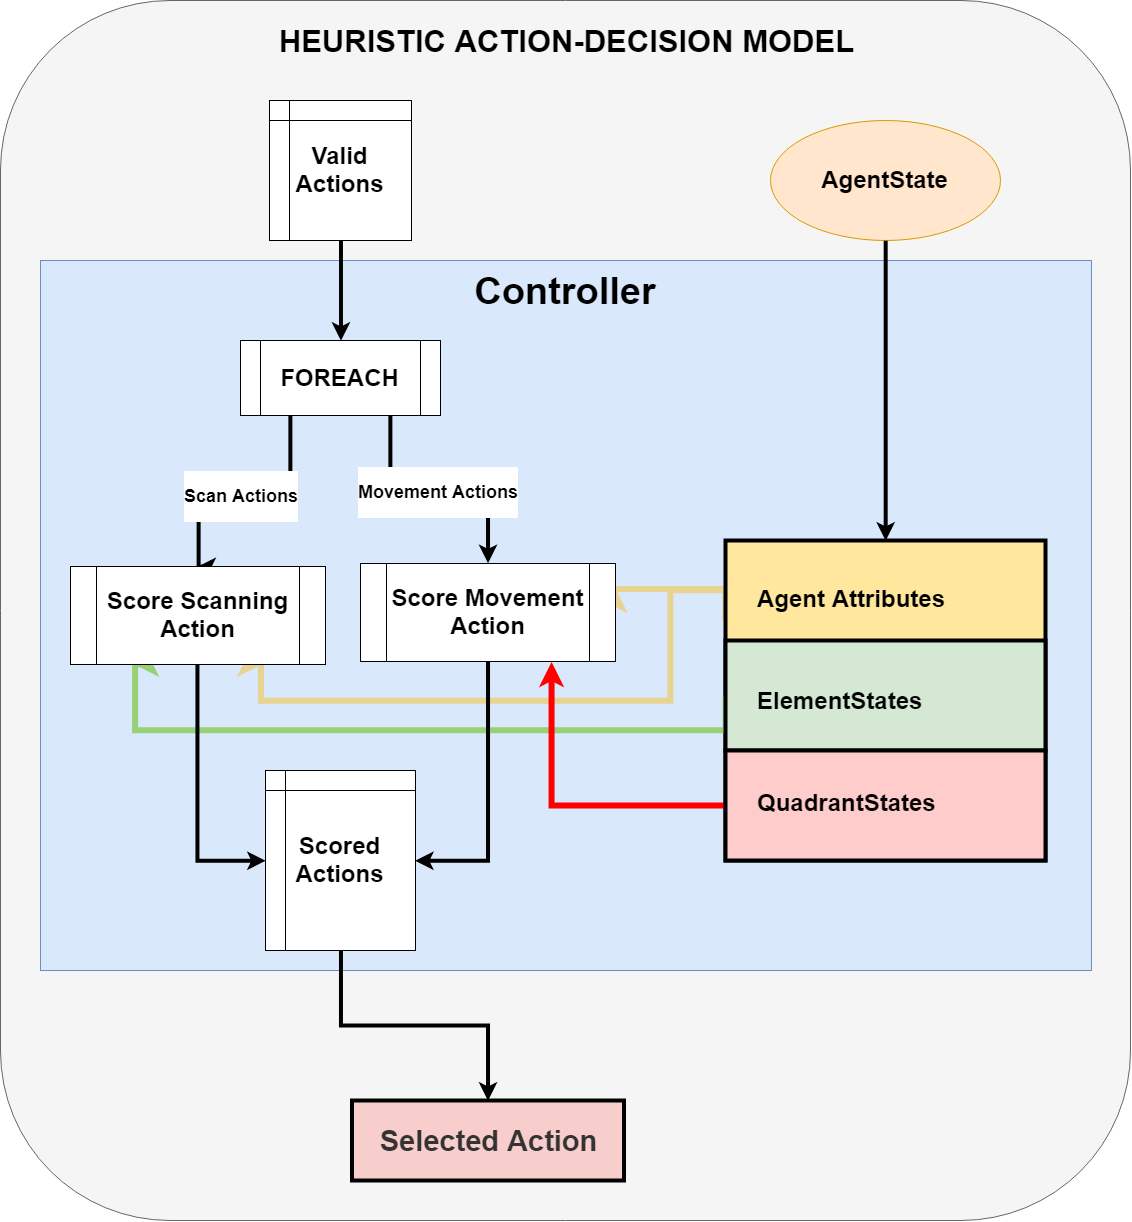
\includegraphics[width=1.0\columnwidth]{Figures/heuristic_decision_model.png}
  \caption[Heuristic Control Model]{The general decision model that our heuristic controllers follow. An \texttt{AgentState} and a list of valid actions are passed to the controller. The controller then assigns a score to each action by analyzing related attributes within the \texttt{AgentState}. The highest scoring action is then returned.}
  \label{fig:heuristic_decision_model}
\end{figure}

Valid scanning actions are all scored using function~\ref{algorithmic:score_scan_action}.
Higher scores will be given to scanning actions for an element type that is considered more important and has fewer known values within the corresponding sensor's range.
Importance of an element type is determined by whether it is flagged as hazardous and/or as an indicator.
The amount of known values in the corresponding sensor's range is calculated by referencing the agent's \texttt{internalMap}.
The resulting score should influence the controller to use sensors efficiently, assist with hazard avoidance, and emphasize goal completion.

\begin{algorithm}[!htb]
  \setstretch{1.35}
  \caption[Heuristic - Score Potential Scan Action]{Calculate a score for a considered scanning action for a specific element type based on an \texttt{ElementState}. The returned result will be used to rank the action in the decision-making process. $W_{item}$ denotes the attributed weight for $itemReward$.}
  \begin{algorithmic} \label{algorithmic:score_scan_action}
    \REQUIRE $W_{indicator} \in \left[0, \infty \right)$
    \REQUIRE $W_{hazard} \in \left[0, \infty \right)$
    \REQUIRE $W_{pkir} \in \left[0, \infty \right)$
    \REQUIRE $W_{immediates} \in \left[0, \infty \right)$
    \REQUIRE $indicator \in \{true, false\}$
    \REQUIRE $hazard \in \{true, false\}$
    \REQUIRE $percentKnownInRange \in \left[0, 1 \right]$
    \REQUIRE $immediatesKnown \in \left[0, 4 \right]$
    \ENSURE $scanActionScore \in \left[0, 1 \right]$
    \IF {indicator = true}
      \STATE $iScore \leftarrow W_{indicator}$
    \ELSE
      \STATE $iScore \leftarrow 0$
    \ENDIF
    \IF {hazard = true}
      \STATE $hScore \leftarrow W_{hazard}$
    \ELSE
      \STATE $hScore \leftarrow 0$
    \ENDIF
    \STATE $pkirScore \leftarrow (1 - percentKnownInRange) \times W_{pkir}$
    \STATE $imdsScore \leftarrow ((4 - immediatesKnown) / 4) * W_{immediates}$
    \STATE $scoresTotal \leftarrow iScore + hScore + pkirScore + imdsScore$
    \STATE $W_{total} \leftarrow W_{indicator} + W_{hazard} + W_{pkir} + W_{immediates}$
    \RETURN $scanActionScore \leftarrow scoresTotal / W_{total}$
  \end{algorithmic}
\end{algorithm}


Scoring each valid movement actions is based on the controller's specific implementation of the \texttt{scoreMovmentAction} function.
These functions involve a series of sub-functions tied to each available sensor's element type.
Each of the sub-functions calculate a sub-score for their element type.
These sub-functions use threshold analyses on the \texttt{QuadrantState}s corresponding to the direction of movement being considered.
Once each element type's sub-score has been returned to the \texttt{scoreMovmentAction} function, an overall score is determined by a weighted average.
The overall scoring functions used for $Heuristic_{FH}$ (algorithm~\ref{algorithmic:findHuman_scoreMovmentAction}) and $Heuristic_{MW}$ (algorithm~\ref{algorithmic:mapWater_scoreMovementAction}) follow the same logic, but contain different sub-functions and related weights.
For an example of how threshold analyses are conducted within a sub-function, see $Heuristic_{FH}$'s \texttt{scoreElevation} algorithm (algorithm~\ref{algorithmic:findHuman_scoreElevation}).


\begin{algorithm}[!htb]
  \setstretch{1.35}
  \caption[Heuristic - Score Potential Movement Action (Find Human)]{Calculate a score for a considered movement action in a specific direction based on a set of corresponding \texttt{QuadrantState}s ($QS$). The returned results will be used to rank the action in the decision-making process. $W_{item}$ denotes the attributed weight for $itemReward$. This function also uses a $score<Element-Type>$ function. Example for one such equation is algorithm~\ref{algorithmic:findHuman_scoreElevation}. This equation is used specifically for the $Heuristic_{FH}$ controller's decision model.}
  \begin{algorithmic} \label{algorithmic:findHuman_scoreMovmentAction}
    \REQUIRE $W_{elevation} \in \left[0, \infty \right)$
    \REQUIRE $W_{decibel} \in \left[0, \infty \right)$
    \REQUIRE $W_{temperature} \in \left[0, \infty \right)$
    \REQUIRE $W_{water} \in \left[0, \infty \right)$
    \ENSURE $scoreElevation \rightarrow \left[0, 1 \right]$
    \ENSURE $scoreDecibel \rightarrow \left[0, 1 \right]$
    \ENSURE $scoreTemperature \rightarrow \left[0, 1 \right]$
    \ENSURE $scoreWater \rightarrow \left[0, 1 \right]$
    \ENSURE $movementActionScore \in \left[0, 1 \right]$
    \STATE $eScore \leftarrow scoreElevation(QS) * W_{elevation}$
    \STATE $dScore \leftarrow scoreDecibel(QS) * W_{decibel}$
    \STATE $tScore \leftarrow scoreTemperature(QS) * W_{temperature}$
    \STATE $wScore \leftarrow scoreWater(QS) * W_{water}$
    \STATE $scoresTotal \leftarrow eScore + dScore + tScore + wScore$
    \STATE $W_{total} \leftarrow W_{elevation} + W_{decibel} + W_{temperature} + W_{water}$
    \RETURN $movementActionScore \leftarrow scoresTotal / W_{total}$
  \end{algorithmic}
\end{algorithm}


\begin{algorithm}[!htb]
  \setstretch{1.35}
  \caption[Heuristic - Score Potential Movement Action (Map Water)]{Calculate a score for a considered movement action in a specific direction based on a set of corresponding \texttt{QuadrantState}s ($QS$). The returned results will be used to rank the action in the decision-making process. $W_{item}$ denotes the attributed weight for $itemReward$. This function also uses a $score<Element-Type>$ function. Example for one such equation is algorithm~\ref{algorithmic:findHuman_scoreElevation}. This equation is used specifically for the $Heuristic_{MW}$ controller's decision model.}
  \begin{algorithmic} \label{algorithmic:mapWater_scoreMovementAction}
    \REQUIRE $W_{elevation} \in \left[0, \infty \right)$
    \REQUIRE $W_{water} \in \left[0, \infty \right)$
    \ENSURE $scoreElevation \rightarrow \left[0, 1 \right]$
    \ENSURE $scoreWater \rightarrow \left[0, 1 \right]$
    \ENSURE $movementActionScore \in \left[0, 1 \right]$
    \STATE $eScore \leftarrow scoreElevation(QS) * W_{elevation}$
    \STATE $wScore \leftarrow scoreWater(QS) * W_{water}$
    \STATE $scoresTotal \leftarrow eScore + wScore$
    \STATE $W_{total} \leftarrow W_{elevation} + W_{water}$
    \RETURN $movementActionScore \leftarrow scoresTotal / W_{total}$
  \end{algorithmic}
\end{algorithm}


\begin{algorithm}[!htb]
  \setstretch{1.35}
  \caption[Heuristic - Score Quadrant (Elevation)]{Calculate a score for a \texttt{QuadrantState} ($Q$) of element type ``elevation.'' The returned results will be used to rank the action in the decision-making process. $W_{item}$ denotes the attributed weight for $itemReward$. This equation is used in both the $Heuristic_{FH}$ and $Heuristic_{FH}$ controllers' decision models.}
  \begin{algorithmic} \label{algorithmic:findHuman_scoreElevation}
    \REQUIRE $W_{percentKnown} \in \left[0, \infty \right)$
    \REQUIRE $W_{immediateValue} \in \left[0, \infty \right)$
    \ENSURE $percentKnown \rightarrow \left[0, 1 \right]$
    \ENSURE $scanMovementScore \in \left[0, 1 \right]$
    \STATE $pkScore \leftarrow scoreElevation(QS) * W_{elevation}$
    \IF {$\exists immediateValue$}
      \IF {$|immediateValue| > 12$}
        \STATE $imScore \leftarrow 1$
      \ELSE
        \STATE $imScore \leftarrow 0$
      \ENDIF
    \ELSE
      \STATE $imScore \leftarrow 0$
    \ENDIF
    \STATE $scoresTotal \leftarrow pkScore + imScore$
    \STATE $W_{total} \leftarrow W_{elevation} + W_{decibel} + W_{temperature} + W_{water}$
    \RETURN $scanActionScore \leftarrow scoresTotal / W_{total}$
  \end{algorithmic}
\end{algorithm}


\section{SCOUt Controller} \label{sec:scout_controller}
The SCOUt controller uses reinforcement learning to build a memory of past actions and rewards for planning future actions.
After each operation, the SCOUt controller will store state-action rewards in memory.
A state-action reward (SAR) contains the action that the agent took, the state that the agent was in when it chose this action, and the short-term and long-term rewards that the agent received.
In future operations, the SCOUt controller (figure~\ref{fig:scout_decision_model}) will search in memory to find SARs with states that are similar to the agent's current state.
Utilizing data from the agent's current state and the controller's collection of past action-state pairs, SCOUt will predict rewards for each possible action and select one based on these predictions.

\begin{figure}[!htb]
  \centering
  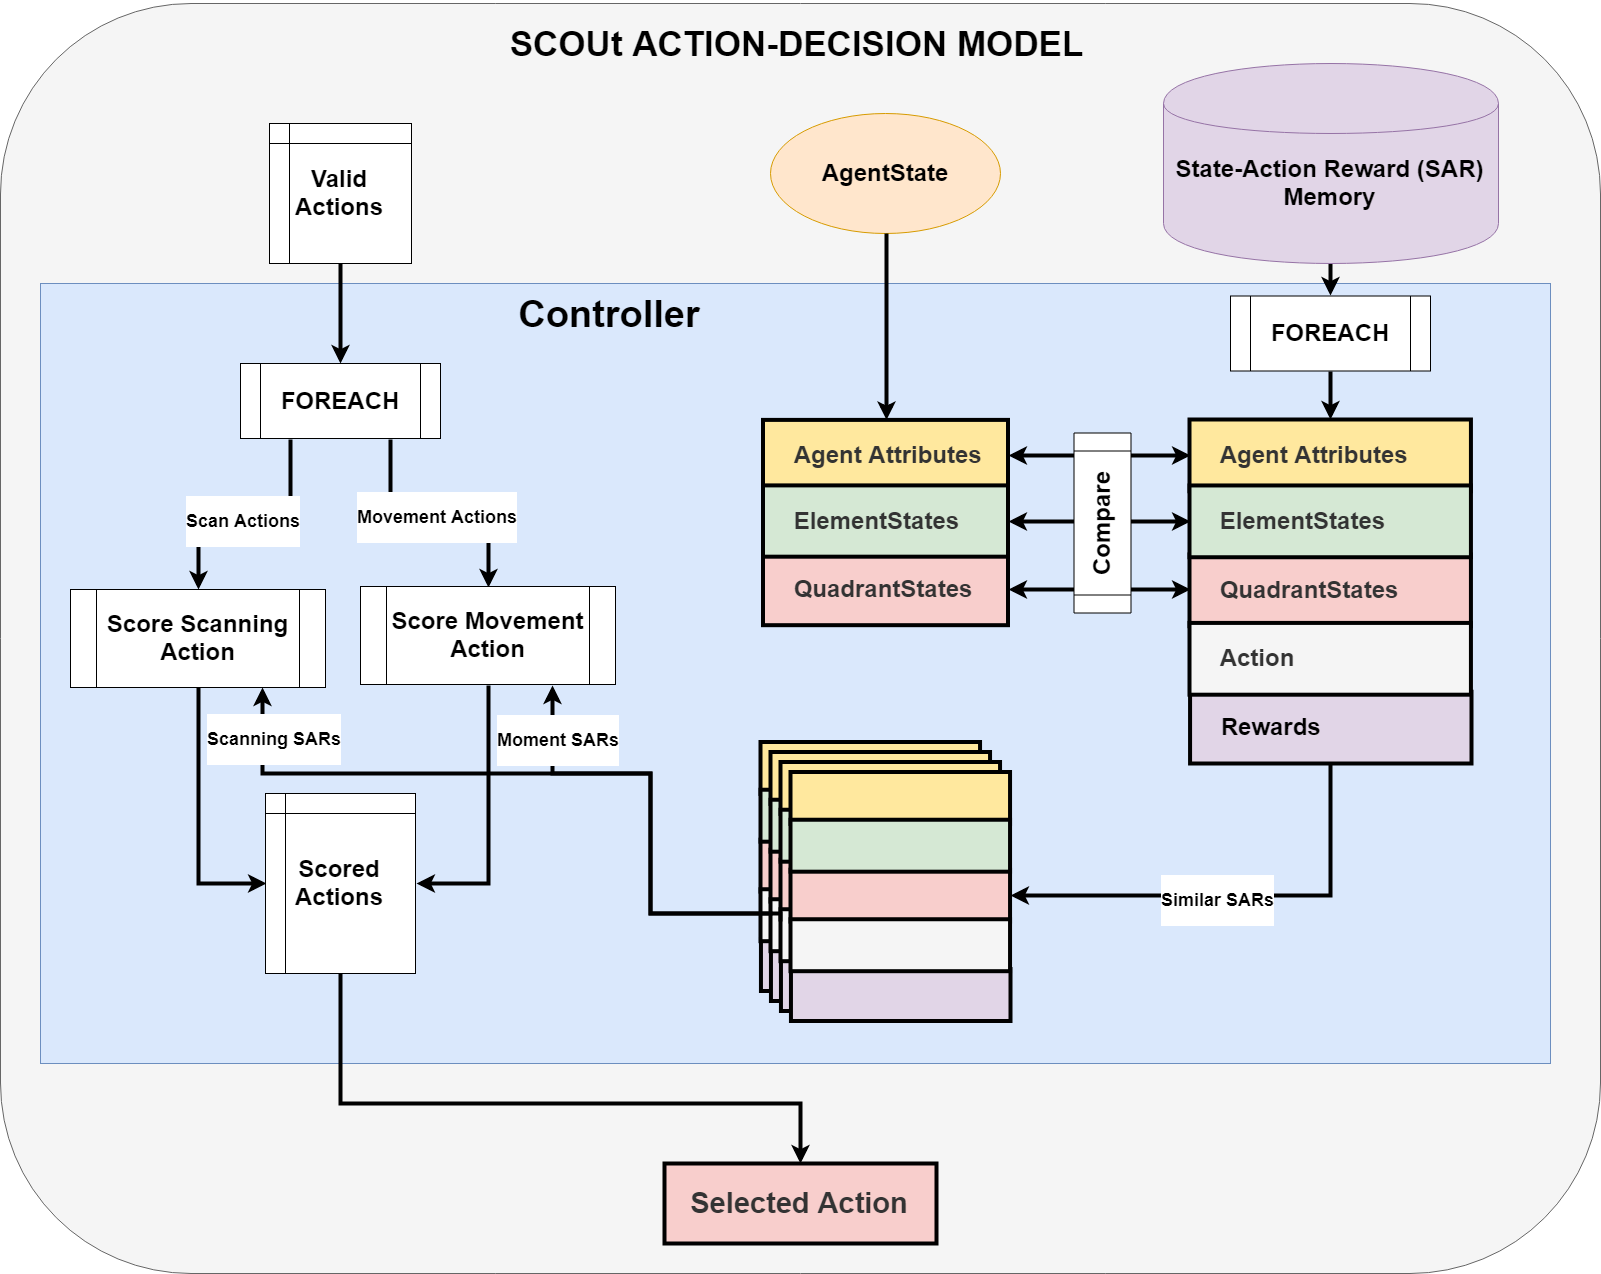
\includegraphics[width=1.0\columnwidth]{Figures/scout_decision_model.png}
  \caption[SCOUt Control Model]{Action decision model for the SCOUt controller. The controller searches for memory state-action rewards (SAR) that have a similar state to the current state. The chosen actions and rewards for each similar SAR is used to create a score for each valid action that the can be taken in the current state.}
  \label{fig:scout_decision_model}
\end{figure}

Calculations used for action decision rely on several weights and variables to assist in state comparisons and future reward prediction.
Because of the large number of weights required for these calculations, a basic genetic algorithm (GA) was used to optimize these weights.
The GA initialized a population of 10 weight sets and evolved them for 50 generations.
Each generation creates five mutated copies and five crossover copies of individuals in the current population.
The individuals that are copied for mutation or crossover are chosen using roulette selection.
% \todo{ref roulette selection algo}
% \todo{ref GA algo}
Fitness scores are calculated for each of the resulting 20 individuals based on their performance within a series of 50 operations.
Ten survivors are then selected for the next generation.
Survivor selection keeps the two individuals with the highest fitness scores and uses roulette selection for choosing the remaining seven.
The weight set with the highest fitness in the final generation was selected for use in experimentation, and its values listed in table ~\ref{table:evolved_weight_set}.

% \todo{sizing}
\begin{table}
  \centering
  % \small
  \def\arraystretch{1.25}
  \caption[Variables and Weights]{Set of variables and weights used by the SCOUt controller for action decision. These variables/weights were produced using a basic genetic algorithm.}
  \resizebox{\textwidth}{!}{%
  \begin{tabular}{ l l c }
    \hline
    \textbf{Attribute}                & \textbf{Description}            & \textbf{Variable/Weight} \\
    \hline
                                      & \textbf{State Comparison Weights}& \\
    health                            & remaining health               & 0.41  \\
    energy                            & energy level                & 0.78  \\
    elementStates                     & overall element states                & 0.61  \\
    quadrantStates                    & overall quadrant states                & 0.16  \\
    \hline
                                      & \textbf{Element State Comparison Weights}& \\
    indicator                         & element type is indicator                & 0.31  \\
    hazard                            & element type is hazardous                & 0.07  \\
    percentKnownInRange               & known element type values in range of sensor                & 1.0   \\
    immediateKnown                    & number of immediate cell values known                & 0.41  \\
    \hline
                                      & \textbf{Quadrant State Comparison Weights}& \\
    indicator                         & element type is indicator                & 0.38  \\
    hazard                            & element type is hazardous                & 0.23  \\
    percentKnown                      & known element type values in quadrant                & 0.2   \\
    averageValue                      & average element value in quadrant cells                & 0.19  \\
    immediateValue                    & immediate quadrant cell value                & 0.29  \\
    \hline
                                      & \textbf{Action Selection}& \\
    similarityThreshold               & SAR comparison qualification  & 0.26  \\
    minimumSimilarStates              & used to calculate prediction ``confidence''    & 10    \\
    repetitionPenalty                 & penalty for action that would be repetitive                & 0.1   \\
    \hline
                                      & \textbf{Movement Action Score Weights}& \\
    predictedShortTermReward          & action's predicted short-term reward       & 0.87  \\
    predictedLongTermReward           & action's predicted long-term reward      & 0.45  \\
    confidence                        & confidence in predicted rewards       & 0.25  \\
    \hline
                                      & \textbf{Scanning Action Score Weights}& \\
    predictedShortTermReward          & action's predicted short-term reward       & 0.61  \\
    predictedLongTermReward           & action's predicted long-term reward      & 0.34  \\
    confidence                        & confidence in predicted rewards       & 1.0   \\
    \hline
  \end{tabular}}
  % \caption{Table ~\ref{table:evolved_weight_set}: Evolved Weight Set}
  \label{table:evolved_weight_set}
\end{table}


\subsection{Memory}
The SCOUt controller can gather memory from every operation.
When an operation has finished, and long-term rewards have been assigned to each action, the controller creates new SARs, and selects a sub-set of them to be stored in memory.
The rest are discarded.
Saving only a sub-set cuts back on the size of the memory file as well as the computational time that will be required to search for similar states.
The current memory selection method in this project's implementation saves the last 20 SARs, and a uniformly sampled sub-set of the remaining SARs from the operation.
The last 20 are always saved because they typically hold the most important events leading up to the success or failure of the operation.
To also capture events that occur during the agent's initial and intermediate search process, the controller retains 5 percent of the remaining SARs generated.
These SARs are uniformly sampled beginning at index 0.
So, if there were 100 SARs in the remaining set, SARs indexed 0, 20, 40, 60, and 80 would be stored in memory.
Each SAR is added to the controller's memory file as a JSON object.
The next time that the controller is used in operation, the collection of SARs can then be decoded from the file back into \texttt{StateActionReward} class instances.


\subsection{State Normalization}
The data within each SAR's state is relative to the operation in which they were recorded.
To handle variances found between all of the states stored in memory, SCOUt normalizes them using a Gaussian approach as suggested by McCaffrey~\cite{mccaffrey_how_nodate}.
Normalization helps make data values more meaningful when studied by the controller.
For example, if the controller was seeking out a human, it may look for increases in decibel values.
In order for the controller to determine how much of an increase is significant enough to investigate, it needs to first understand what variations are considered normal.
Gaussian distribution provides this functionality through the calculation of mean and standard deviation ($sd$) values in a data set.
If the agent has gathered decibel readings in its north quadrant that are well outside the $sd$ found in the controller's memory, it should be encouraged to investigate.
All numerical attributes within an \texttt{AgentState} are normalized using this Gaussian method.
This applies to health and \texttt{energyLevel} within \texttt{AgentState}s, \texttt{percentKnownInSensorRange} within \texttt{ElementState}s, and \texttt{percentKnown}, \texttt{averageValueDifferential}, and

\noindent
\texttt{immediateValueDifferential} within \texttt{QuadrantState}s.

The normalization process begins by extracting each of these attributes from all SAR states within the loaded memory.
Next the mean and standard deviation values are calculated and stored in an instance of a \texttt{GuassianData} class (Appendix~\ref{appendix:gaussian_data}).
Once mean and standard deviation values are known, the controller will go back through every SAR's state and normalize their attributes using each corresponding \texttt{GaussianData} class instance.
The normalization function (equation~\ref{eq:gaussian_normalize}) will produce a ``normal'' value that reflects how many standard deviations the attribute falls above or below the mean.
A value of 0 represents no difference between the attribute's value and the mean, values of 1 and -1 represent a difference of one standard deviation from the mean, and so on.
When SCOUt searches for similar states, it will also normalize the current state using the existing \texttt{GuassianData} instances.
By normalizing the current state against the states in memory, the numerical attributes compared will all be relative to the mean of the values held in memory.

\begin{capeq}
  \begin{equation} \label{eq:gaussian_normalize}
    x_{normal} = \frac{(x - m)}{sd}
  \end{equation}
  \caption[Value Normalization]{Normalization of an attribute value, $x$, based on the gaussian mean, $m$, and gaussian standard deviation, $sd$, for the given attribute.}
\end{capeq}


% \todo{major revisions to this section}
% Replace as much as possible with graphics
% \todo{eliminate weighted average refs?}

\subsection{State Comparisons} \label{subsec:state_comparisons}
Now that all state attributes are normalized, the controller can use a more intuitive approach for calculating the differences between two states.
State comparisons are used to build a set of SARs from memory that contain states similar to an agent's current state.
These SARs will later be used to assist in reward prediction.
For an SAR to qualify for addition into this set, its state must have an overall difference below the \textit{similarityThreshold} specified in table ~\ref{table:evolved_weight_set}.
Overall state difference is calculated using a series of difference calculations between related attributes in the two compared \texttt{AgentState}s.
Results from the series of difference calculations will all be collapsed into a single \textit{overallStateDifference} using a weighted average function (equation ~\ref{eq:weighted_average}).
By comparing each attribute separately and applying a weighted average to the resulting difference calculations, this allows the controller to assign a level of importance to each individual attribute.
Importance is assigned via weight values that are between 0 and 1 (see ``state comparison'' weights in table~\ref{table:evolved_weight_set}).
The higher the attribute's weight it, the more influence it will have in the overall state difference.
An attribute with a weight of 0 will be completely ignored in a weighted average equation.
Different weighted average equations are used for \textit{overallStateDifference} calculation depending on whether the considered SAR's action is a movement or scanning action.
This allows the controller to compare only the attributes that are relevant to the type of action that was selected.

\begin{capeq}
  \begin{equation} \label{eq:weighted_average}
    WeightedAverage = \frac{\sum_{i=0}^{n} A_{i} * W_{i}}{\sum_{i=0}^{n} W_{i}}
  \end{equation}
  \caption[Weighted Average]{A general equation that takes a list of $n$ attribute values ($V$) and a list of $n$ corresponding weights ($W$) and calculates a weighted average of all attribute values.}
\end{capeq}

Difference comparisons for each attribute in an \texttt{AgentState} are calculated based on their data type (boolean, normalized numerical value, optional normalized numerical value, or sub-class).
Sub-class comparisons, such as comparing two \texttt{ElementState}s, follow the same procedure as \texttt{AgentState} does for calculating an overall difference.
Difference comparisons will be made for each of the attributes within the sub-class, and a weighted average function is applied to the results.
Boolean differences will return 0 when the compared attributes are both true or both false and return 1 otherwise (equation ~\ref{eq:boolean_difference}).
For example, \textit{BooleanDifference} is used to calculate whether an element type in two \texttt{ElementState}s were both flagged as an indicator or not.
Normalized numerical attributes follow the \textit{GaussianDifference} equation (equation ~\ref{eq:gaussian_difference}).
This equation will produce values that hold the same principle as the normalization process, where the closer the difference is to 0, the more similar they are.
If two values are identical, their \textit{GaussianDifference} will be 0.
Otherwise, the \textit{GaussianDifference} will be relative to how many standard deviations away from each other the two values are.
% Proofs for these behaviors are found in appendix item~\ref{appendix:gaussian_difference_identical} and appendix item~\ref{appendix:gaussian_difference_different} respectively.
Optional values follow a unique case-based equation (equation~\ref{eq:option_difference}) to calculate the \textit{GuassianDifference} only when both are known.
If one value is known and the other is not, a difference of 1 is returned.
If both values are unknown a difference of 0 is returned.

\begin{capeq}
\begin{equation} \label{eq:boolean_difference}
  BooleanDifference = \begin{cases}
    x = y & 0 \\
    x \neq y & 1
  \end{cases}
\end{equation}
\caption[Boolean Difference]{Difference calculation for two boolean values, $x$ and $y$.}
\end{capeq}

\begin{capeq}
\begin{equation} \label{eq:gaussian_difference}
  GaussianDifference = |x_{normal} - y_{normal}|
\end{equation}
\caption[Gaussian Difference]{Difference calculation for two normalized vales, $x$ and $y$.}
\end{capeq}

\begin{capeq}
\begin{equation} \label{eq:option_difference}
  optionDifference =
  \begin{cases}
    x \quad \text{known} \cap y \quad \text{known} & GaussianDifference(x,y) \\
    x \quad \text{known} \oplus y \quad \text{known} & 1 \\
    x \quad \neg \text{known} \cap y \quad \neg \text{known} & 0
  \end{cases}
\end{equation}
\caption[Option Difference]{A difference calculation used for two values ($x$ and $y$), when their values are not always known.}
\end{capeq}

Comparisons with SAR's whose chosen action was a scanning action will apply a weighted average to the health, energy, and element states of the two \texttt{AgentState}s.
Each \texttt{ElementState} within the current \texttt{AgentState} will calculate their own weighted average based on the number of the immediately adjacent cells that are known, the percent of known element values in range of the sensor, the hazard and indicator flags.
All of these \textit{elementStateDifference}s will be averaged (non-weighted) into a single difference value, \textit{averageElementStateDifference}.
This compares the usage of the element type (hazard and/or indicator detection), and knowledge of the element type (percent known within the environment).
The \textit{hazard} and \textit{indicator} differences can help the controller determine the usage of the element type's data being collected.
The \textit{percentKnown} and \textit{immediateValuesKnown} differences help the controller decide whether use of an element type's sensor is efficient or necessary.
For example, if an agent does not have knowledge of the elevation in adjacent cells, it couldn't confidently determine whether it is safe or possible to move into one of those cells without first scanning to find out.

% \begin{capeq}
%   \begin{align*}
%   \begin{equation} \label{eq:scanning_overall_difference}
%     &V = \{health_{diff},\quad energy_{diff},\quad elementStates_{diff}\} \\
%     &W = \{health_{wight},\quad energy_{wight},\quad elementStates_{wight}\} \\
%     &\\
%     &OverallDifference_{s} = WeightedAverage(V,W)
%   \end{equation}
% \end{align*}
% \caption{Calculation for the overall state difference when the compared state-action reward had chosen a scanning action, where $V$ is a list of attributes values and $W$ is the list of weights for the attributes.}
% \end{capeq}

% \begin{capeq}
% \begin{equation} \label{eq:element_state_difference}
% % \begin{align*}
%   &V = \{indicator_{diff},\quad hazard_{diff},\quad percentKnownInRange_{diff},\quad immediateKnown_{diff}\} \\
%   &W = \{indicator_{wight},\quad hazard_{wight},\quad percentKnownInRange_{wight},\quad immediateKnown_{weight}\} \\
%   &\\
%   &elementStateDifference = WeightedAverage(V,W)
% % \end{align*}
% \end{equation}
% \caption{Calculation for the overall difference of two \texttt{ElementState}s, where $V$ is a list of attributes values within the \texttt{ElementState}s and $W$ is the list of corresponding weights.}
% \end{capeq}

If the SAR's action type is movement, overall state difference is calculated using differences in each \texttt{AgentState}s' health, energy, element states, and quadrant states.
In addition to calculating \textit{elementStateDifference}s, \textit{quadrantToQuadrantDifferences} are calculated between every quadrant in the current state and every quadrant in the SAR state.
Only one ``orientation'' of quadrant-to-quadrant comparisons will be used in the overall difference calculation.
Four orientations are considered by rotating the SAR's quadrants in 90 degree intervals (see figure ~\ref{fig:quadrant_orientations}).
The resulting orientation comparisons are denoted as North-to-North, North-to-West, North-to-South and North-to-East (based on the SAR's quadrant that is matched to the current state's North quadrant).
The orientation that yields the lowest \textit{quadrantToQuadrantDifferences} (\textit{lowestQuadrantOrientationDifference}) is used in calculating $OverallDifference_{m}$.

% \begin{capeq}
% \begin{equation} \label{eq:movement_overall_difference}
% \begin{align*}
%   &V = \{health_{diff},\quad energy_{diff},\quad elementStates_{diff},\quad quadrantStates_{diff}\} \\
%   &W = \{health_{wight},\quad energy_{wight},\quad elementStates_{wight},\quad quadrantStates_{weight}\} \\
%   &\\
%   &OverallDifference_{m} = WeightedAverage(V,W)
% \end{align*}
% \end{equation}
% \caption{Calculation for the overall state difference when the compared state-action reward had chosen a movement action, where $V$ is a list of attributes values and $W$ is the list of weights for the attributes.}
% \end{capeq}

\begin{figure}[!htb]
  \centering
  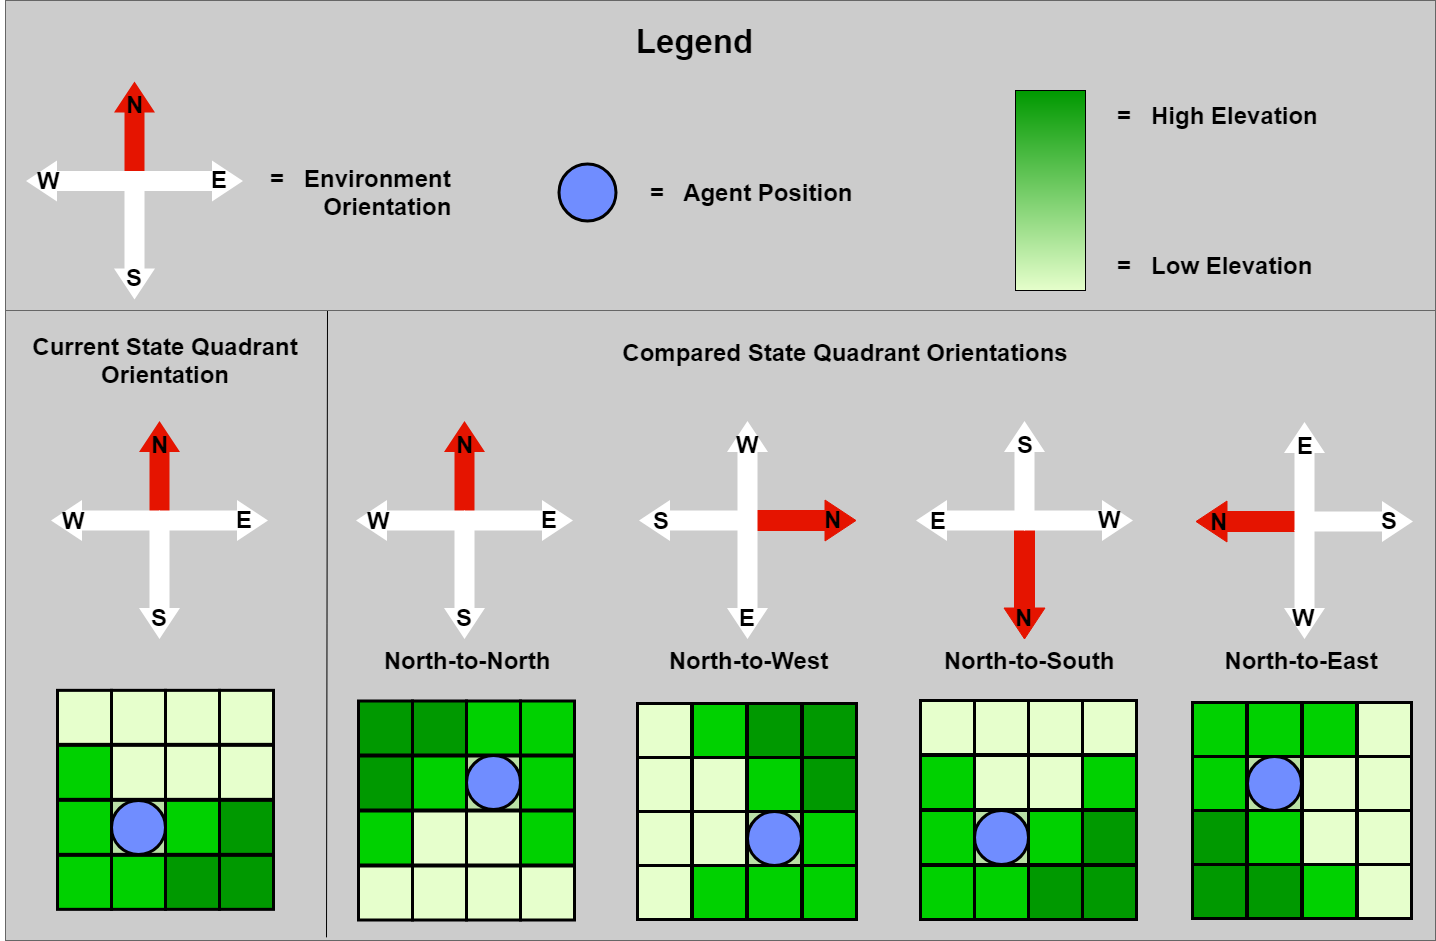
\includegraphics[width=1.0\columnwidth]{Figures/quadrant_orientations.png}
  \caption[State Comparison Orientations]{Orientation considerations between two compared states. This displays how rotating the compared environment's quadrant orientation can reveal states of higher similarity. We see that the elevation heatmaps of the two are highly similar when compared at North-to-South orientation, where as an un-altered quadrant comparison (North-to-North) would yield a very negative comparison.}
  \label{fig:quadrant_orientations}
\end{figure}

Each orientation is important to consider because the controller is only concerned with moving towards interesting features in an environment, regardless of the direction.
Considering the orientation with the lowest difference makes the comparison relative to the two environments instead of the cardinal direction.
Consider if a highly similar SAR held information that its agent received good rewards for a particular movement action.
The current agent should be encouraged to move towards the quadrant in its own environment that holds similar features (not necessarily in the same direction).
Now, if the SAR's \textit{lowestQuadrantOrientationDifference} is found when rotating its quadrants 180 degrees (North-to-South orientation) and it had chosen to move East, the current agent should choose to move West since the two states are oriented at a 180 degree difference between each other (see figure ~\ref{fig:oriented_movement_example}).

\begin{figure}[!htb]
  \centering
  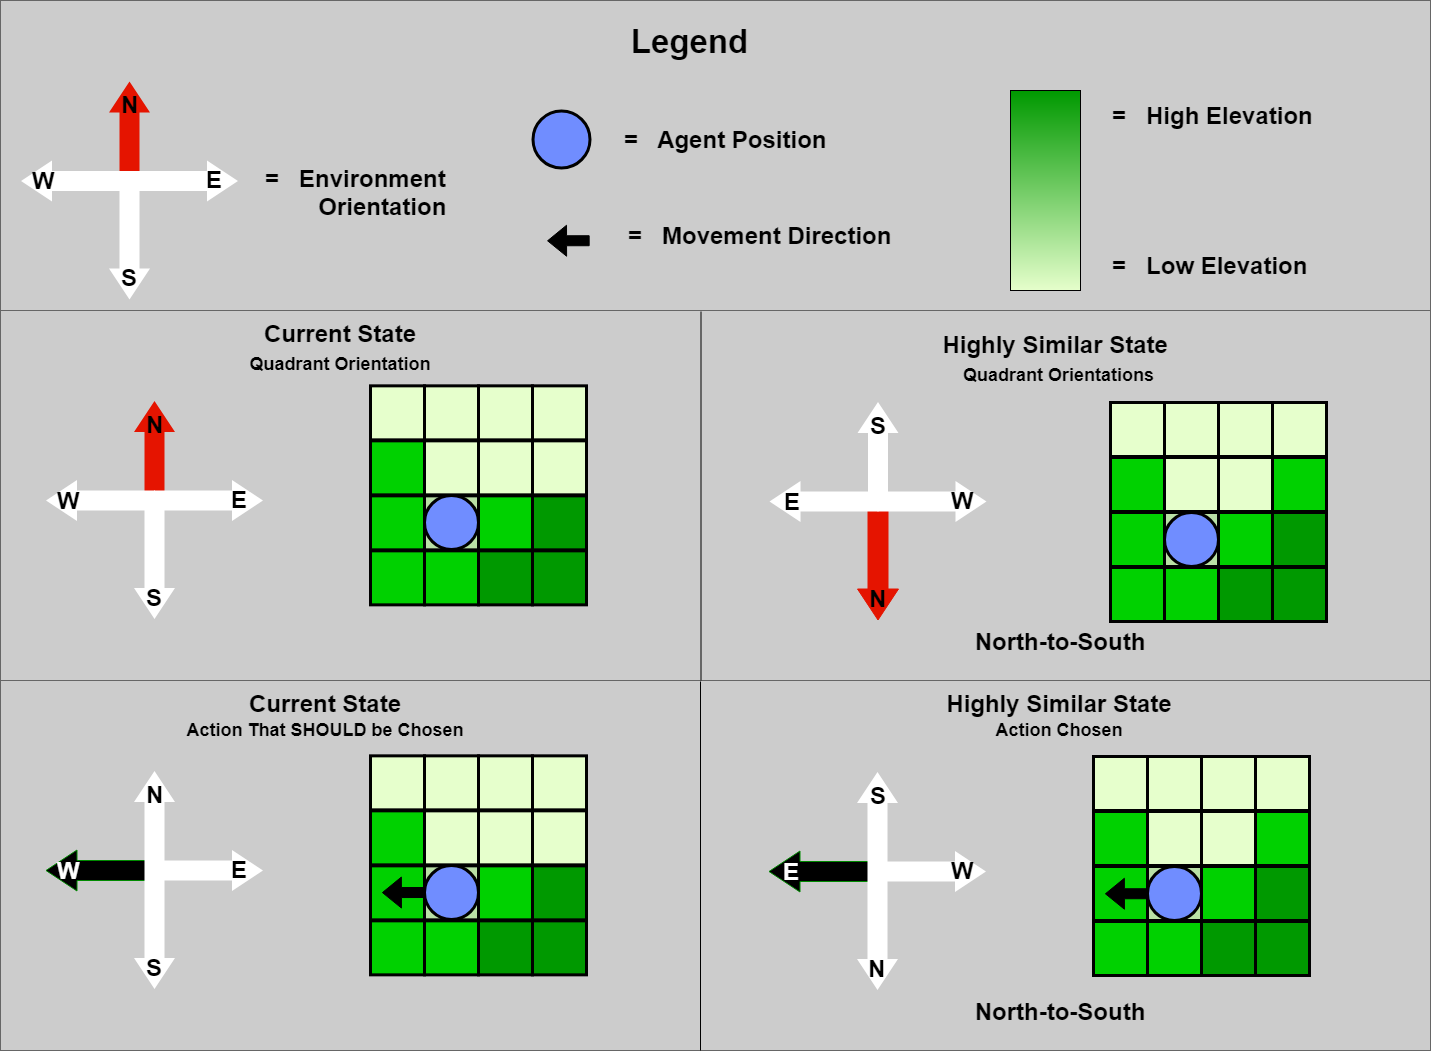
\includegraphics[width=1.0\columnwidth]{Figures/oriented_movement_example.png}
  \caption[Orientation Comparison Example]{Example of two states that have a \textit{lowestQuadrantOrientationDifference} at North-to-South orientation. The display exemplifies how after finding the most similar orientation, the action taken by the compared state must also be re-oriented to match the \textit{lowestQuadrantOrientationDifference}. In doing so the agent will be considering movement relative to the matching features in the environment.}
  \label{fig:oriented_movement_example}
\end{figure}

Quadrant-to-quadrant comparisons produce a non-weighted average of \textit{quadrantElementStateDifference}s.
A \textit{quadrantElementStateDifference} is calculated between every \texttt{ElementState} in the current state's considered quadrant and the matching \texttt{ElementState} in the SAR state's considered quadrant (if it exists).
The \textit{quadrantElementStateDifference} uses a weighted average to compare attributes within the two \texttt{ElementState}s' considered quadrants.
For example, making a North-to-South quadrant comparison would consider element types in the current state's North quadrant against element types in the SAR's South quadrant.
When making these comparisons, it is not guaranteed that the current state and SAR state will share all the same element types.
For example, if the current state contains decibel data and the SAR state does not, no comparison can be made, and it will receive a \textit{quadrantElementStateDifference} of 1.
Because we are only comparing against element types in the current \texttt{AgentState}, if the SAR contains any element types not present in the current state, they are simply ignored.
These comparisons examine how much information about the element type is known, and the actual values in the quadrants (if they are known).
Because \texttt{averageValueDifferential} and \texttt{immediateValueDifferential} are not guaranteed to be known values for every quadrant, they use the unique option difference equation (equation ~\ref{eq:option_difference}).

% \begin{capeq}
% \begin{equation} \label{eq:quadrant_element_state_difference}
% \begin{align*}
%   &V = \{percentKnown_{diff},\quad averageValueDifferential_{diff},\quad immediateValueDifferential_{diff}\} \\
%   &W = \{percentKnown_{wight},\quad averageValueDifferential_{wight},\quad immediateValueDifferential_{wight}\} \\
%   &\\
%   &quadrantElementStateDifference = WeightedAverage(V,W)
% \end{align*}
% \end{equation}
% \caption{Calculation for comparing the difference between two \texttt{ElementState}s in given quadrants, where $V$ is a list of attributes values and $W$ is the list of weights for the attributes.}
% \end{capeq}

Once all sub-differences have been calculated and either $OverallDifference_{s}$ or $OverallDifference_{m}$ is known, the controller can decide whether the SAR qualifies to be used in future reward prediction for the current agent.
If the calculated overall difference is below the \textit{similarityThreshold}, the SAR will qualify and an instance of the \texttt{StateActionDifference} class (Appendix~\ref{appendix:state_action_difference}) is created.
Each instance stores the overall difference value, the SAR's action taken, and the short-term and long-term rewards.
State comparison will be repeated for every SAR in the memory pool, and the resulting collection of \texttt{StateActionDifference} instances is passed to the action reward prediction algorithm.



\subsection{Action Reward Prediction}
Once the controller has generated a set of \texttt{StateActionDifference}s (SAD), it will predict a short-term and long-term reward value that each possible action might receive, along with a confidence score for the predictions.
For each valid action considered, the algorithm will select a sub-set of SAD where the \texttt{StateActionDifference}'s \texttt{action} is the same as the one being considered.
Predicted short-term and long-term rewards are calculated as an average of all the \texttt{shortTermScore}s and \texttt{longTermScore}s in the sub-set.
Confidence is evaluated using the average of the \texttt{overallStateDifference}s in the sub-set, weighted by the number of \texttt{StateActionDifference}s in the sub-set (equation~\ref{eq:confidence}).
The equation will invert \textit{overallStateDifference}s when averaging them by subtracting their value from 1 (equation~\ref{eq:diff_to_similarity}).
This allows the prediction algorithm to look at them as ``similarity'' scores instead of ``difference'' scores.
If the overall difference had been 0 (the states compared were identical), their similarity score will be 1.
Because \textit{similarityThreshold} was used to filter out SARs with high overall difference values, it can be asserted that the average of all \textit{overallStateDifference}s will not fall below: $1 - similarityThreshold$.
The prediction algorithm then computes an overall \textit{actionScore} for each action using a weighted average of the predicted short-term reward, predicted long-term reward, and the confidence score.

\begin{capeq}
\begin{equation} \label{eq:diff_to_similarity}
  similarity = 1 - difference
\end{equation}
\caption[Difference to Similarity Inversion]{Equation for inverting an \textit{overallStateDifference} value to create a similarity value. The minimum \textit{overallStateDifference} that can exist is 0. By this logic, the highest attainable similarity between two states is 1.}
\end{capeq}

\begin{capeq}
\begin{equation} \label{eq:confidence}
  confidence = \begin{cases}
    n = 0 & 0 \\
    n < minimumSimilarStates & \frac{\sum_{n}^{i=0} 1 - SAD_{i}.overallStateDifference}{minimumSimilarStates} \\
    n >= minimumSimilarStates & \frac{\sum_{n}^{i=0} 1 - SAD_{i}.overallStateDifference}{n} \\
\end{cases}
\end{equation}
\caption[Reward Prediction Confidence]{Confidence value assigned to reward prediction values based on a set of $n$ \texttt{StateActionDifference}s ($SAD$), and the $minimumSimilarStates$ value from the evolved weight set (table ~\ref{table:evolved_weight_set}).}
\end{capeq}

% \begin{capeq}
% \begin{equation} \label{eq:action_score}
% \begin{align*}
%   &V = \{predictedShortTermReward,\quad predictedLongTermReward,\quad confidence\} \\
%   &W = \{predictedShortTermReward_{weight},\quad predictedLongTermReward_{weight},\quad confidence_{weight}\} \\
%   &\\
%   &actionScore = WeightedAverage(V,W)
% \end{align*}
% \end{equation}
% \caption{Action scoring function using the action's $predictedShortTermReward$, $predictedLongTermReward$, and $confidence$, in pairing with their corresponding weights found in table ~\ref{table:evolved_weight_set}}
% \end{capeq}


\subsection{Action Selection}
Once every valid action has received an \textit{actionScore}, there are two methods the controller may use for choosing which one the agent should perform.
If the controller is being trained, roulette selection is used.
Roulette selection is an integral part of training as it will give every action a chance to be selected.
This will fill the controller memory with a variety of events both good and bad, giving the reward prediction algorithm more concise data to work with.
When the controller is being used outside of training, the action with the highest score is always selected.
Once selected, the agent will then attempt to perform the action, and its interaction with the environment will be reflected in a new \texttt{AgentState}.
If the agent is still operational after the resulting event and the goal has not yet been completed, the action decision process (figure ~\ref{fig:scout_decision_model}) will begin again using the new \texttt{AgentState}.
Once the agent is no longer operational, or the goal has been completed, the operation process ends, and new SARs are added to the controller's memory file.







% \todx{style algo}
% \begin{lstlisting}
% 1. Normalize the current state (how many SDs it falls outside of the average)
% 2. Calculate the Gaussian difference for:
%   a. health
%   b. energyLevel
%   c. elementStateDifferences = for each element state:
%     i. hazardDifference = if (current == SAR) 1 else 0
%     ii. indicatorDifference = if (current == SAR) 1 else 0
%     iii. percentKnownInSensorRangeDifference = abs(SAR - current)
%     iv. immediateValuesKnownDifference = abs(SAR - current) / 4
%   d. quadrantToQuadrantStateDifferences = for each current quadrant:
%     i. quadrantStateDifferences = for each SAR quadrant:
%       a. quadrantElementStateDifferences = for each element type:
%         i. hazardDifference = if (current == SAR) 1 else 0
%         ii. indicatorDifference = if (current == SAR) 1 else 0
%         iii. percentKnownDifference = abs(SAR - current)
%         iv. averageValueDifferentialDifference = if (current known && SAR known) abs(SAR - current) else (if current known == if SAR knonw) 1 else 0)
%         v. immediateValueDifferentialDifference = if (current known && SAR known) abs(SAR - current) else (if current known == if SAR knonw) 1 else 0)
% 3. Sum all differences together using weighted values for each Gaussian difference.
%   a. Movement state difference
%   b. Scan state difference
% \end{lstlisting}



% \subsection{Action Reward Prediction}
% Action reward prediction first calculates three factors for each valid action being considered: predicted short term reward, predicted long term reward and confidence.
% These factors are determined by StateActionDifference that hold the same action as the current action whose reward is being predicted.
% Only a list of similar StateActionDifferences are considered in these calculations.
% This list is made up of StateActionDifferences with an overall difference below a the set minDifferenceThreshold.
% Predicted short and long term rewards are calculated by the average of short and long term scores within the list of similar StateActionDifferences.
%
% If there are no StateActionDifferences in the list, the action being considered will receive a predicted short term reward and long term reward of 0.5 and a confidence of 0.


% An action's short and long term rewards are predicted from the averages of SARs where: A) the considered action was selected, and B) the state difference from the current state is below a certain threshold.
% In addition to these predicted rewards, we also calculate a confidence value for the predictions.
% \tods{confidence EQ}
% The lower the difference is between the current and SAR states, the higher the confidence will be.
% Additionally, the more SARs that are considered in the prediction, the more confident the controller can be in the predicted reward.



\chapter{EXPERIMENTS AND RESULTS} \label{ch:experiments_and_results}
To analyze the SCOUt control schema, three instances of a SCOUt controller are trained and then tested in two experiments.
The first experiment compares the performance of each SCOUt controller against a random and heuristic controller to determine if they exhibit intelligent behavior when attempting to complete a given goal.
The second experiment tests adaptability of the controllers by removing sensors or changing the goal and providing additional training for new goals.
This will create new situations for which the controllers have not been trained.
Two different goals are used in these experiments: \textit{Find Human} and \textit{Map Water}.
\textit{Find Human} requires the agent to search an environment to locate a \texttt{Human} anomaly randomly placed within the environment.
\texttt{Human} is an extended class of the \texttt{Anomaly} trait, and its definition can be found in Appendix~\ref{appendix:human_class}.
Goal completion is either 100 percent for successfully locating the human, or 0 percent for failing to find the human before health or energy has been depleted.
For the goal to be successfully completed, the controller must navigate to one of the eight cells adjacent to the Human anomaly's location in the environment (figure~\ref{fig:human_discovery_zone}).
\textit{Map Water} tests a controller's ability to navigate within an environment and collect as much water depth data as possible.
\textit{Map Water} operations will run until the entire area has been scanned for water depth, or the agent has depleted its health or energy.
Goal completion is then reward based on the percentage of the environment that was scanned for water depth.
Training and testing are both conducted using three different \texttt{EnvironmentTemplates}.
Templates differs in their difficulty to navigate due to the modifications present within them.
For example, more difficult templates will generate larger environments to explore that contain more hazardous terrain modifications.

\begin{figure}[H]
  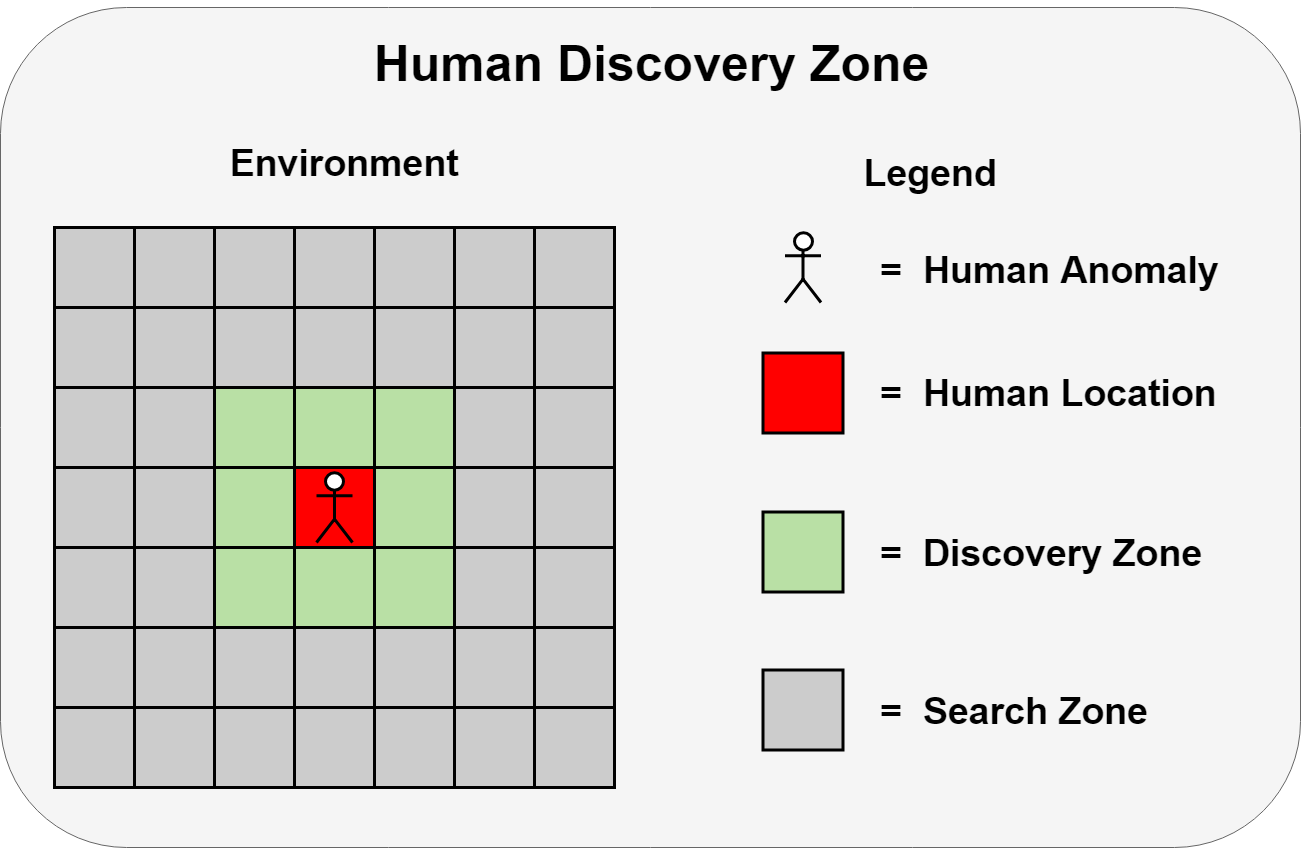
\includegraphics[width=0.8\columnwidth]{Figures/human_discovery_zone.png}
  \caption{Diagram of the area in an environment that an agent must navigate to in order to ``discover'' a human anomaly. This applies to operations where the goal is \textit{Find Human}.}
  \label{fig:human_discovery_zone}
\end{figure}

% \todo{testing fig}

During both training and experimentation, tests are conducted to measure the performance of each controller.
A test is a series of operations that an agent will attempt to complete using a given set of sensors.
Each operation in the series will be run once per controller, where each run is identical: same goal, same environment instance, same starting position, and same agent setup (aside from the controller that is used).
The only exception to this is in Experiment 2 (section~\ref{sec:experiment2}), when sensors are removed from the SCOUt controller's agent to test adaptability.
Tests will measure the performance of several controllers in these identical operations to see how they compare.
Each test will include at least one random, one heuristic and one SCOUt controller.
Two different heuristic controllers are used in testing depending on the goal of the operation.
$Heuristic_{FH}$ and $Heuristic_{MW}$ are used for \textit{Find Human} and \textit{Map Water} operations, respectively.
The random and heuristic controllers provide baselines for performance of the SCOUt controllers.
These baselines are important as the difficulty of an operation is difficult to predict.
Different instances of the same operation setup can yield unique environments and starting positions that will alter the difficulty of goal completion, or even prevent it entirely.
Performance is measured in four categories: goal completion, the number of actions taken, remaining health and remaining energy.
Additionally, the agent's starting location for each operation will be chosen in a location that does not result in damage (e.g., starting in a cell with water present) or immediate goal completion (e.g., starting next to the Human anomaly).
The specific agent setups and \texttt{EnvironmentTemplates} used for training and experimentation are covered in sections~\ref{sec:agent_setups} and~\ref{sec:test_environment_templates}.


\section{Agent Setup} \label{sec:agent_setups}
% \todo{diagram}
A similar agent setup is used for every operation in training and testing.
The only variation is in the controller being used and the sensor types present.
All health, energy, mobility and durability variables will be set to the same value throughout training and experimentation.
This will ensure that no advantage or disadvantage is given to any controller when navigating the agent through an environment.
The performance of each controller will then solely be reflected by their usage of available sensors, and analyses of the data they collect.
Different sensors are available for use depending on the goal, or in the unique case where the set of equipped sensors are changed tests in Experiment 1 (section~\ref{sec:sensor_change}), depending on the test setup.
Four sensors are used throughout testing: elevation, temperature, decibel and water.
When sensors are available for an agent to use, the indicator flag will reflect their usage for the present goal.
For \textit{Find Human} the temperature and decibel sensors will be flagged as indicators, and for \textit{Map Water} the water sensor will be flagged as an indicator.
Water and elevation sensors are always flagged as hazard since the defined agent \texttt{Durability} and \texttt{Mobility} instances make the agent susceptible to water and fall damage.
Each Agent will always begin an operation with an empty \texttt{internalMap}, 100.0 \texttt{health} and a starting \texttt{energyLevel} of 100.0.
The instances of the \texttt{Agent}, \texttt{Mobility}, \texttt{Durabilities}, and each \texttt{Sensor} used in training and testing are found in Appendix~\ref{appendix:agent_setup}.


\section{Environment Templates} \label{sec:test_environment_templates}
Three \texttt{EnvironmentTemplate}s with increasing difficulty are created for use in training and experimentation (\textit{EASY}, \textit{MEDIUM}, and \textit{HARD}).
Change in difficulty is achieved by adjusting: environment size, presence of \texttt{TerrainModification}s, average and deviation values of each \texttt{ElementSeed}, and the values within each \texttt{Effect} of any \texttt{Anomaly} present.
Increased environment size creates a wider area that an agent will have to explore.
More \texttt{TerrainModification}s makes each environment potentially more hazardous.
Hills and valleys can create areas with the potential of fall damage or the inability to climb slopes, and pools and streams of water will create areas that will damage an agent that enters them.
Changing the average and deviation values of \texttt{ElementSeed}s used to generate the \texttt{Environment} instance has a couple of effects.
As an example, by increasing the average decibel values in the environment, the distinction of the human's decibel \texttt{Effect} is dampened, and the agent will need to navigate closer to the source in order to detect any noise produced.
Also, if the variance in decibel values increases, it becomes more difficult for an agent to distinguish what levels of increase are considered significant enough to investigate.
Last, by adjusting the values within \texttt{Anomaly} \texttt{Effect}s, it can become harder for an intelligent controller to detect the \texttt{Anomaly} from a distance.
For example, by reducing the decibel effect of a \texttt{Human Anomaly}, the radiation of the effect will cover less area in the environment, meaning the agent will have to search longer before it may pick up on the effect.

Each environment template has one \texttt{Human} that will be placed into it at random in a non-hazardous zone.
The same templates will then be used for both the \textit{Find Human} and \textit{Map Water} goals.
In the case that the goal is \textit{Map Water}, a \texttt{Human Anomaly} will still be present within the environment, but it will be ignored by the agent.
Each of these \texttt{EnvironmentTemplate}s are listed in JSON format in Appendix~\ref{appendix:experiment_setup}.
When a template is used in training or experimentation, it will be loaded from its file, converted to a Scala object, and passed to the \texttt{EnvironmentBuilder}.
The resulting \texttt{Environment} instance can then be used in one or more test operations.


\section{Training} \label{sec:training}
Three separate SCOUt controllers are trained to accumulate memory pools of state-action rewards.
Each of the three controllers are trained with different goal configurations but follow the same training process (figure~\ref{fig:training_diagram}).
One is trained using the \textit{Find Human} goal, the second using the \textit{Map Water} goal and the third is a hybrid, trained using both goals.
They are named $SCOUt_{FH}$, $SCOUt_{MW}$ and $SCOUt_{H}$ respectively.
Each controller is trained for 30 iterations, where an iteration runs one operation per environment template.
Once training has completed, each controller will have collected state-action rewards (SAR) from a total of 90 operations (30 on EASY, 30 on MEDIUM and 30 on HARD).
Every operation that $SCOUt_{FH}$ is run in will be with the \textit{Find Human} goal and every operation for $SCOUt_{MW}$ will be with the \textit{Map Water} goal.
$SCOUt_{H}$ will alternate goals for each iteration.
In total it will have run 45 operations with the \textit{Find Human} goal and 45 operations with the \textit{Map Water} goal (15 on EASY, 15 on MEDIUM and 15 on HARD for each).

\begin{figure}[h]
  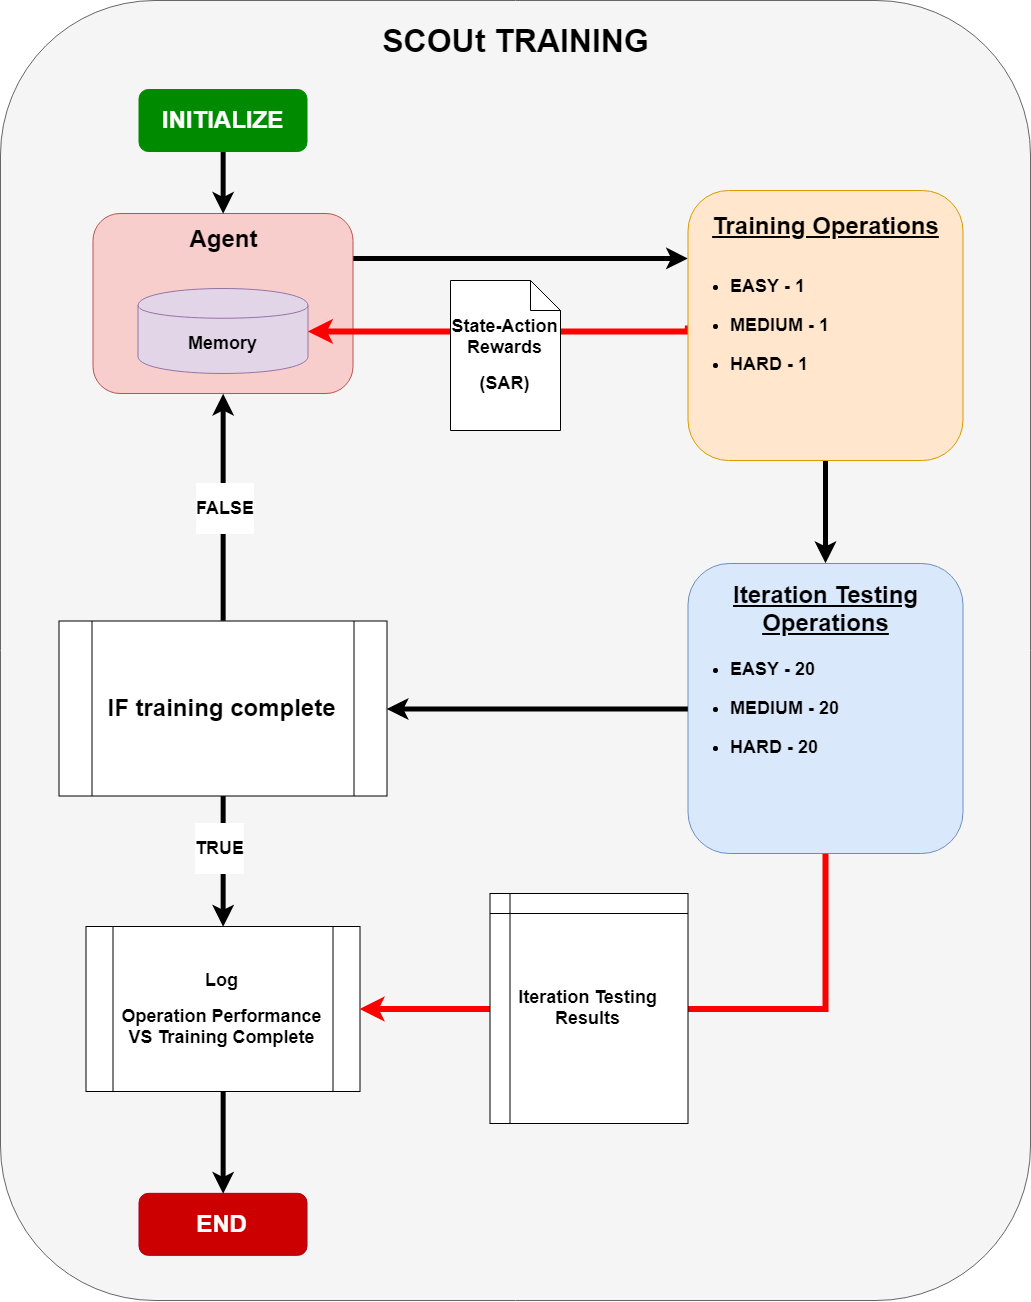
\includegraphics[width=1.0\columnwidth]{Figures/training_diagram.png}
  \caption{This diagram shows the training process that each SCOUt controller will follow. Training is completed after 30 iterations of the process. The number of operations for each environment difficulty in training and in iteration testing are shown. The goal for the operation will depend on the specific SCOUt controller that is being trained.}
  \label{fig:training_diagram}
\end{figure}

After each training iteration, the controller is tested with its current memory to track performance improvements.
Testing at each iteration runs a series of simulated operations to collect performance data.
Each series uses the controller's respective goal(s) and is run on each testing environment template 20 times (20 on EASY, 20 on MEDIUM, and 20 on HARD).
The controller tested will have access to its current memory pool that it has gathered during all of the training operations it has completed so far.
As the purpose of iteration testing is to measure the \textit{current} performance level of the controller, no SARs will be gathered during these tests and the memory will be left un-altered.
For a baseline, the $Random$ controller is run through the same series of tests.
Results from the 60 total operations will be averaged in each of the four performance categories.
The averaged results of the learning SCOUt controller will then be differenced against the averaged results of the $Random$ controller.
By differencing the averages, we are observing how much better or worse the SCOUt controller was able to perform than the $Random$ controller in the same testing conditions.
This also removes the discrepancy between each iteration test that is run, as one iteration text may have generated a series of exceptionally difficult or easy operations.
It is expected that as training continues, the goal completion, remaining health and remaining energy performances of SCOUt will increase, and the number of actions performed will decrease when compared against the $Random$ controller.

\subsection{Initial Training Results}
Results for $SCOUt_{FH}$ training (figure~\ref{fig:findhuman_training_results}) show the desired trends of increased performance over training iterations.
Average goal completion and average remaining energy begin at the same performance levels as $Random$ and increase to be consistently better than random over time.
The average number of actions performed begins slightly below $Random$ and continue to decrease before leveling out roughly two-thirds of the way through training.
This demonstrates that the controller is learning to perform more efficiently over time, as both average goal completion and average remaining health show major performance boosts, while fewer actions are being used.
The average remaining health of $SCOUt_{FH}$ shows slight increase over training, but for the most part is equivalent to that of the $Random$ controller.

% \todo{Improve captions}
\begin{figure}[H]
  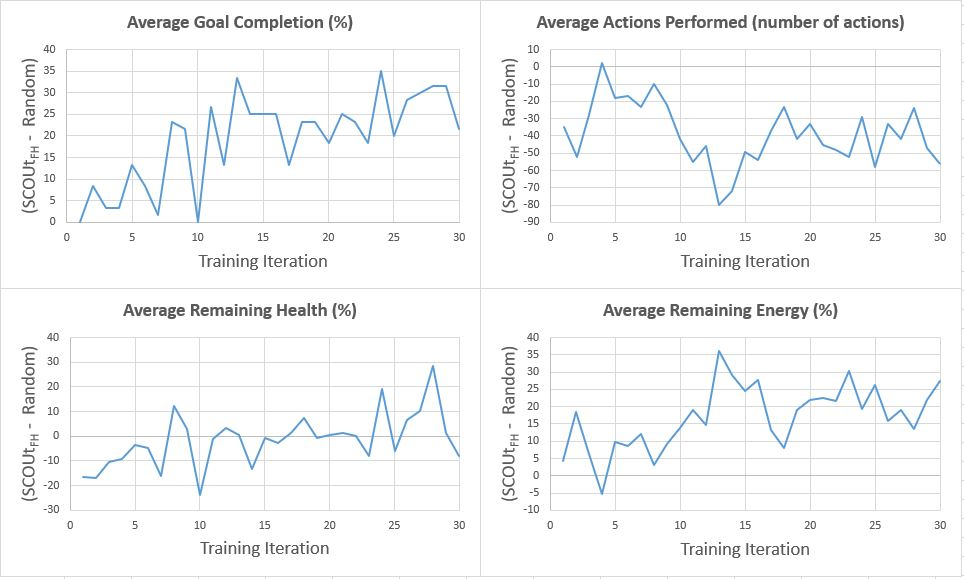
\includegraphics[width=1.0\columnwidth]{Figures/Results/Training/SCOUt-FindHuman.JPG}
  \caption{Iteration testing performance results for $SCOUt_{FH}$ attempting \textit{Find Human}. All graphs show the controller's average difference in performance compared to $Random$ ($SCOUt_{FH}$ average - $Random$ average) VS the number of training iterations completed.}
  \label{fig:findhuman_training_results}
\end{figure}

Results for $SCOUt_{MW}$ (figure~\ref{fig:mapwater_training_results}) are less positive.
Average goal completion and average remaining health both decrease during the first half of training but begin to show upward trends toward the end.
While the average goal completion of $SCOUt_{MW}$ is consistently better than $Random$'s, the average remaining health actually performs worse throughout iteration testing.
$SCOUt_{MW}$ does perform well in the average number of actions taken per operation, however this is likely due to the fact that health is depleted (agent navigating into water) and the operation is ended early.
The same can be said for the remaining energy, as there will be a larger amount of energy remaining after an operation is ended due to depletion of health.
The reason for these poor performance results seem to be tied with the agent's inability to avoid hazardous areas containing water.
Training was repeated using different setups to see if results could be improved.
These repeated training runs are discussed in subsection~\ref{subsec:training_variations}.
Despite unimpressive training results, $SCOUt_{MW}$ still performs well in the tests to follow.

\begin{figure}[H]
  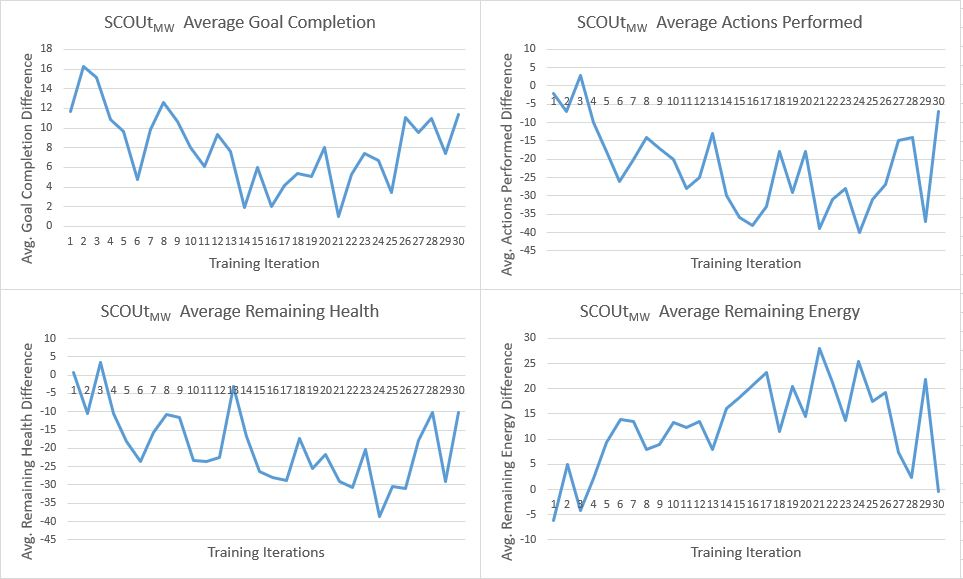
\includegraphics[width=1.0\columnwidth]{Figures/Results/Training/SCOUt-MapWater.JPG}
  \caption{Iteration testing performance results for $SCOUt_{MW}$ attempting \textit{Map Water}. All graphs show the controller's average difference in performance compared to $Random$ ($SCOUt_{MW}$ average - $Random$ average) VS the number of training iterations completed.}
  \label{fig:mapwater_training_results}
\end{figure}

For $SCOUt_{H}$, performance was tracked for both of the \textit{Find Human} and \textit{Map Water} goals.
The iteration test results over training for each of these are found in figure~\ref{fig:hybrid_training_results_fh} and figure~\ref{fig:hybrid_training_results_mw}.
For the majority of the results in both goal types, the average performance of $SCOUt_{H}$ does not show any major increasing trends.
In \textit{Find Human} testing, average goal completion rises and falls throughout training.
The cause of this is unclear but is likely a side effect of simultaneous training on two goals at once.
We also see a slight upward trend in the average number of actions that are being performed, but it does stay under $Random$'s performance throughout.
Towards the end of training, performances in \textit{Map Water} begin to shift in three categories.
Remaining health and number of actions performed shift up, while remaining energy drops, and average goal completion remains fairly consistent.
While more actions are being taken (resulting in the decrease of remaining energy), it appears that $SCOUt_{H}$ is learning better hazard avoidance behaviors as remaining health has increased over time.
$SCOUt_{H}$ training was also repeated to see if results could be improved (covered in subsection~\ref{subsec:training_variations}).


\begin{figure}[H]
  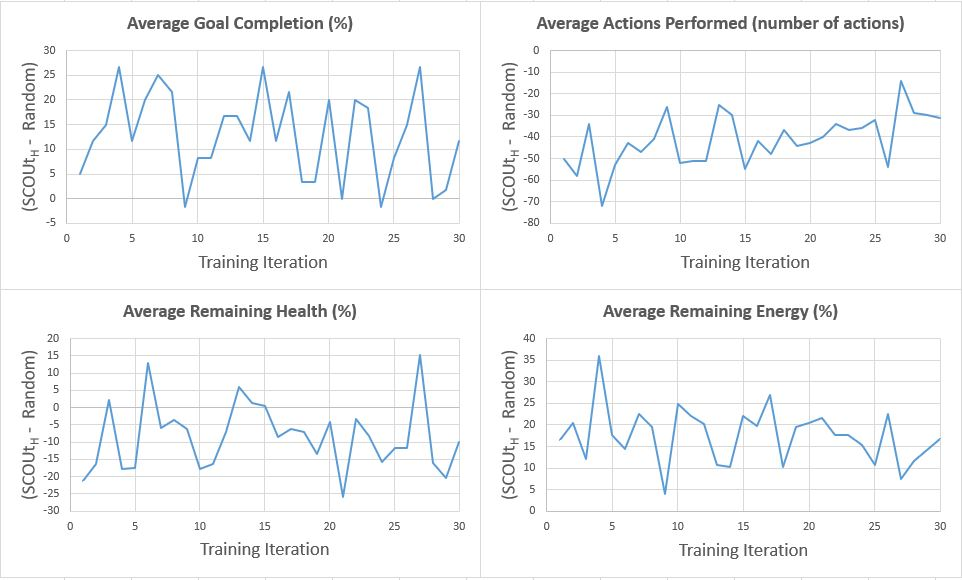
\includegraphics[width=1.0\columnwidth]{Figures/Results/Training/SCOUt-Hybrid-FindHuman.JPG}
  \caption{Iteration testing performance results for $SCOUt_{H}$ attempting \textit{Find Human}. All graphs show the controller's average difference in performance compared to $Random$ ($SCOUt_{H}$ average - $Random$ average) VS the number of training iterations completed.}
  \label{fig:hybrid_training_results_fh}
\end{figure}

\begin{figure}[H]
  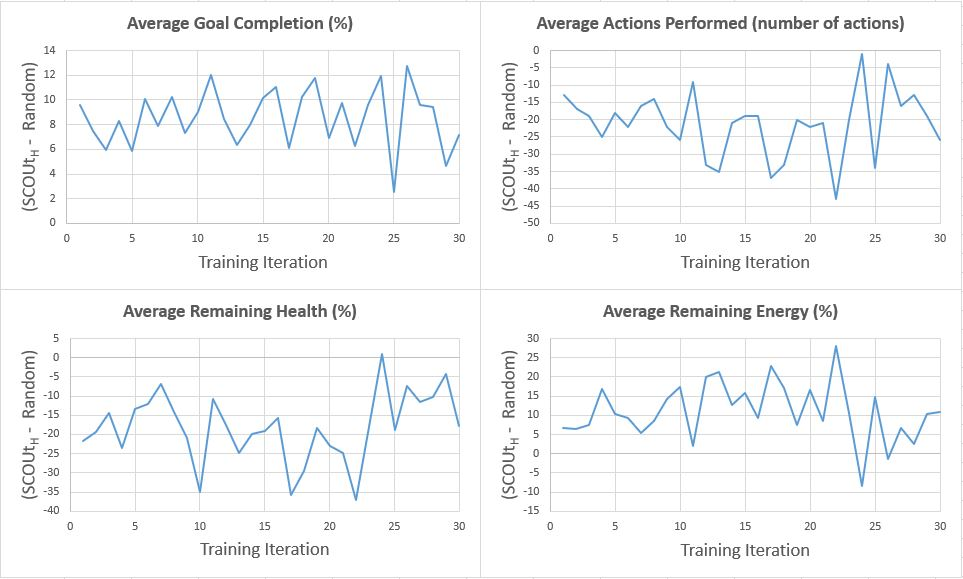
\includegraphics[width=1.0\columnwidth]{Figures/Results/Training/SCOUt-Hybrid-MapWater.JPG}
  \caption{Iteration testing performance results for $SCOUt_{H}$ attempting \textit{Map Water}. All graphs show the controller's average difference in performance compared to $Random$ ($SCOUt_{H}$ average - $Random$ average) VS the number of training iterations completed.}
  \label{fig:hybrid_training_results_mw}
\end{figure}


\subsection{Training Variations} \label{subsec:training_variations}
Two variations of SCOUt controller training were conducted to see if better iteration testing results could be achieved for $SCOUt_{MW}$ and $SCOUt_{H}$.
While $SCOUt_{FH}$ performed well in training, this controller was also retrained using the same variations to assure that there would not be any negative effects to its performance.
The repeated runs altered the way that long-term rewards were calculated at the end of operations, but the same training and iteration testing setup was used: 30 iterations, 1 test on each environment per iteration, 60 operations per iteration test, and iteration testing performance was compared relative to the $Random$ controller.
Variation 1 changed the way that operations factored goal completion into the long-term reward (algorithm~\ref{algorithmic:long_term_reward}).
Instead of always rewarding the controller based on their percent of completion, it would only reward them if the agent had remaining health.
This essentially factors the goal completion as 0 percent if the agent had completely depleted its health.
Effects of this alteration are not expected to cause changes in \textit{Find Human} operations (goal completion is already always 0 unless the human was found), but it should lower the rewards seen in \textit{Map Water} operations since there is typically a portion of the goal completed regardless of how the operation ended.
This variation was made in hope that controllers would learn stronger hazard avoidance behaviors through the harsher long-term reward system.
Variation 2 used the original goal completion equation, but altered the weight used for it.
Instead of \texttt{goalRewardWeight} being set to 1, it was bumped up to 1.5.
This variation was conducted to see if more emphasis was needed on the controllers' level of goal completion within the long-term reward.
If a controller obtained a higher level of goal completion, it must have been able to survive in its environment long enough to do so, which would hopefully counteract the hazard avoidance issue.
Results for all three controllers' in the new training variations are displayed as follows: $SCOUt_{FH}$ - figure~\ref{fig:findhuman_training_comparisons}, $SCOUt_{MW}$ - figure~\ref{fig:mapwater_training_comparisons}, $SCOUt_{H}$ - figures~\ref{fig:hybrid_training_fh_comparisons} and~\ref{fig:hybrid_training_mw_comparisons}.
These graphs show an overlay of the performance results for variation 1, variation 2 and the original training setups that were conducted to easily compare differences between them.
All of the results for variations 1 and 2 can be viewed independently in Appendix~\ref{appendix:additional_figures}.

\begin{figure}[H]
  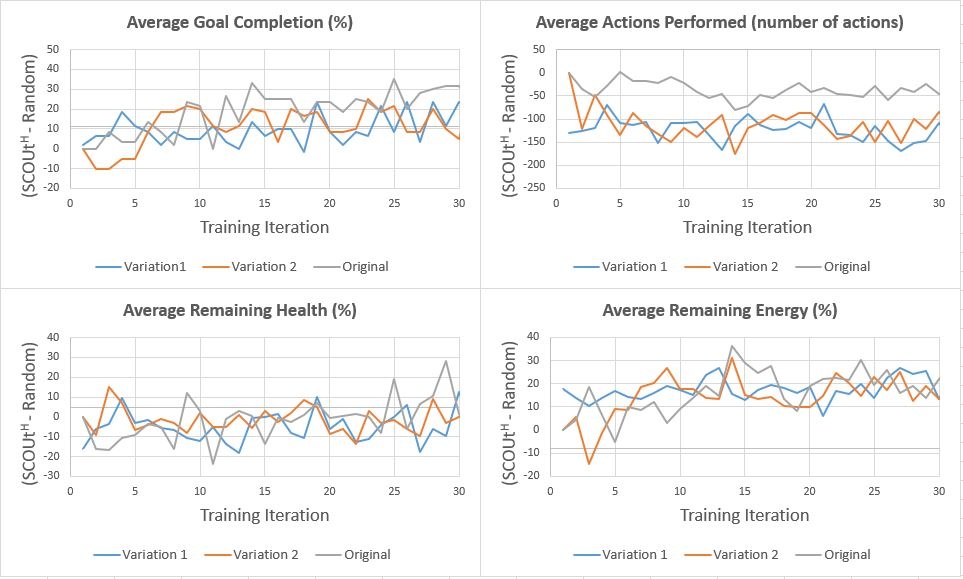
\includegraphics[width=1.0\columnwidth]{Figures/Results/TrainingVariations/FindHuman.JPG}
  \caption{Iteration testing performance results for $SCOUt_{FH}$ attempting \textit{Find Human}. All graphs show the controller's average difference in performance compared to $Random$ ($SCOUt_{FH}$ average - $Random$ average) VS the number of training iterations completed. This graph overlays the results from three different training setups: variation 1, variation 2, and original.}
  \label{fig:findhuman_training_comparisons}
\end{figure}

\begin{figure}[H]
  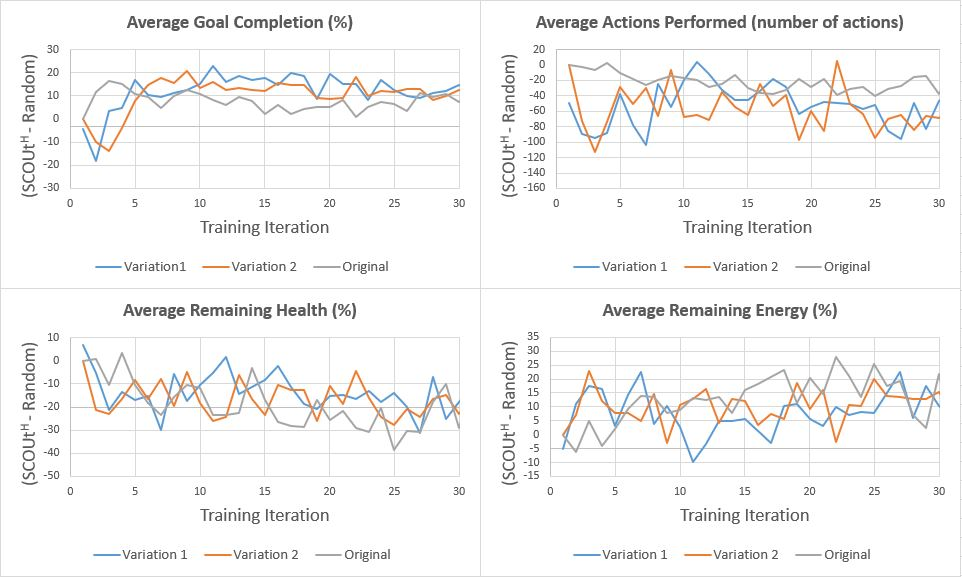
\includegraphics[width=1.0\columnwidth]{Figures/Results/TrainingVariations/MapWater.JPG}
  \caption{Iteration testing performance results for $SCOUt_{MW}$ attempting \textit{Map Water}. All graphs show the controller's average difference in performance compared to $Random$ ($SCOUt_{MW}$ average - $Random$ average) VS the number of training iterations completed. This graph overlays the results from three different training setups: variation 1, variation 2, and original.}
  \label{fig:mapwater_training_comparisons}
\end{figure}

\begin{figure}[H]
  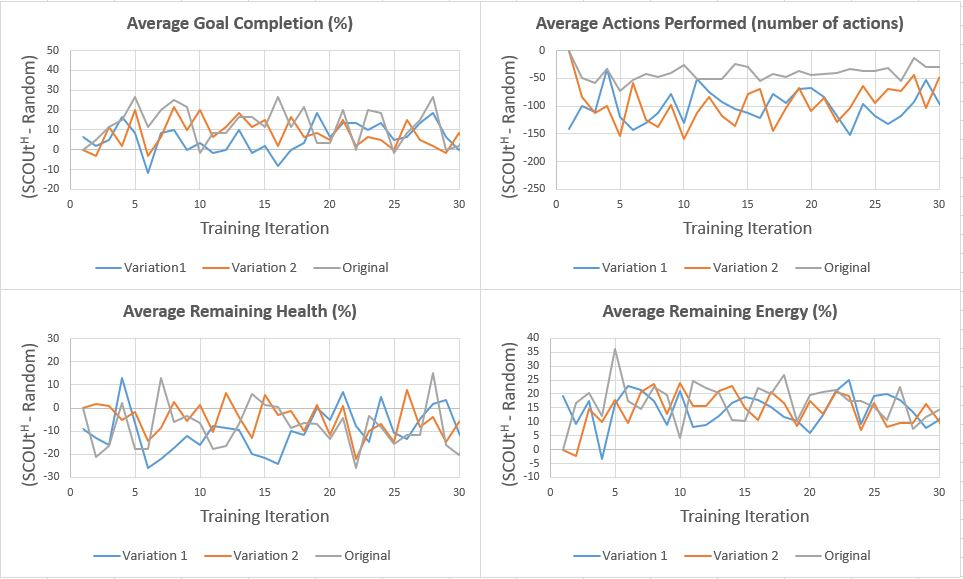
\includegraphics[width=1.0\columnwidth]{Figures/Results/TrainingVariations/Hybrid-FindHuman.JPG}
  \caption{Iteration testing performance results for $SCOUt_{H}$ attempting \textit{FindHuman}. All graphs show the controller's average difference in performance compared to $Random$ ($SCOUt_{H}$ average - $Random$ average) VS the number of training iterations completed. This graph overlays the results from three different training setups: variation 1, variation 2, and original.}
  \label{fig:hybrid_training_fh_comparisons}
\end{figure}

\begin{figure}[H]
  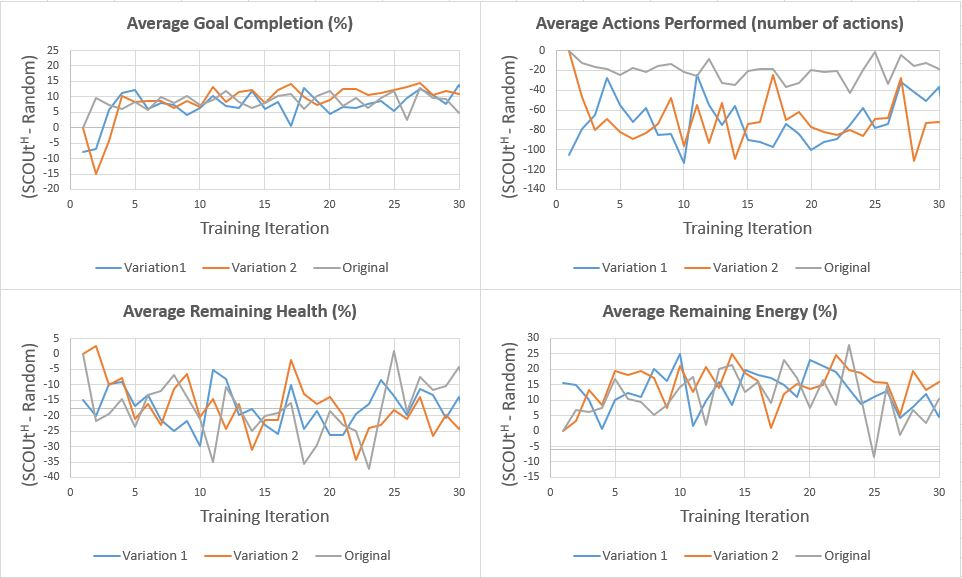
\includegraphics[width=1.0\columnwidth]{Figures/Results/TrainingVariations/Hybrid-MapWater.JPG}
  \caption{Iteration testing performance results for $SCOUt_{H}$ attempting \textit{Map Water}. All graphs show the controller's average difference in performance compared to $Random$ ($SCOUt_{H}$ average - $Random$ average) VS the number of training iterations completed. This graph overlays the results from three different training setups: variation 1, variation 2, and original.}
  \label{fig:hybrid_training_mw_comparisons}
\end{figure}


Performance results show that all of the iteration tests held the same trend lines between each variation of training setup.
Looking at the actual values within each graph, we do see that both variation 1 and 2 hold slightly better results, especially in the category of average actions being performed.
Difference between these two is negligible, so variation 2 was chosen as the winner since it achieved performance boosts through simply adjusting the weighting of goal calculation rather than altering the equation's logic.
For this reason, the following experiments sets the \texttt{goalRewardWeight} to $1.5$ in the long-term reward equation and used the resulting trained memory sets from variation 2 for the SCOUt controllers.



\section{Experiment 1} \label{sec:experiment1}
Once training was completed, the resulting SCOUt controllers were individually tested against $Random$ and their respective heuristic controller.
Tests in Experiment 1 ran a series of 1000 operations per environment template.
The environment template is used to generate 200 unique environments, each of which is used for 5 operations.
Results are averaged for each controller's performance within each of the environment difficulties they were tested in.
We expect to find that the SCOUt controllers perform better than $Random$ and as good or better than the heuristic controllers.
This would be reflected in higher average goal completion, average remaining health and average remaining energy, and lower average actions performed.

Results for $SCOUt_{FH}$ (figure~\ref{fig:findhuman_test_results}) show clear superiority across almost every test.
The only area where scout under-performed was in average remaining health.
In the medium difficulty environments, $SCOUt_{FH}$ came in second in this category (right behind $Heuristic_{FH}$) but all three controllers performed within the same \textasciitilde5 percent range.
In the hard difficulty environments, $SCOUt_{FH}$ came in last out of the three in remaining health, but only by a margin of \textasciitilde2 percent.
Average goal completion in every environment difficulty was about double the performance of $Heuristic_{FH}$ and triple the performance of $Random$.
$SCOUt_{FH}$ also outperformed $Heuristic_{FH}$ and $Random$ in both average actions taken and average remaining health.
We see in these results that the heuristic controller was able to perform better than $Random$ in most tests.
The margin of performance difference between $Heuristic_{FH}$ and $Random$ tends to shrink as the environment difficulty is increased.
While goal completion consistently remained above that of $Random$, we can see that $Heuristic_{FH}$ is having to use more actions to achieve the goal.

\begin{figure}[H]
  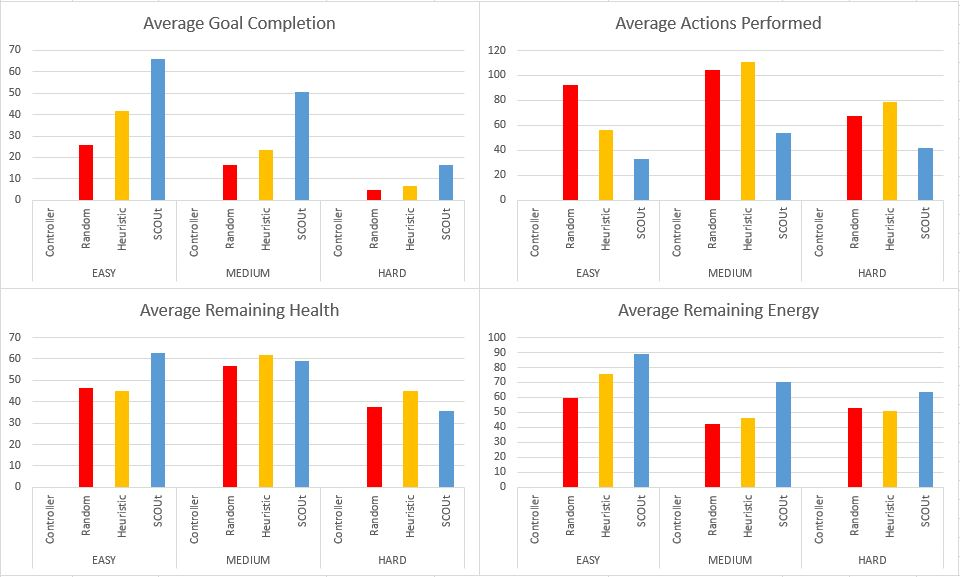
\includegraphics[width=1.0\columnwidth]{Figures/Results/Experiment1/FindHuman.JPG}
  \caption{Performance results for $Random$, $Heuristic_{FH}$ and $SCOUt_{FH}$ controllers attempting \textit{Find Human} in various environment difficulties.}
  \label{fig:findhuman_test_results}
\end{figure}


$SCOUt_{MW}$'s results (figure~\ref{fig:mapwater_test_results}) show performance levels that are mostly superior to $Heuristic_{MW}$ and $Random$, but it does not exhibit the same level of superiority as seen in $SCOUt_{FH}$'s results.
Again, the area where the SCOUt controller is lacking in performance is the average remaining health.
In the easy difficulty environment, $SCOUt_{MW}$ suffers tremendously with an average remaining health of ~9 percent.
Interestingly, the average remaining health increases as environment difficulty increases.
Reasons behind this behavior are unclear as other performance trends increase and decrease as expected when the environment difficulty changes.
$Heuristic_{MW}$ ranks as expected.
The performance values are consistently better than $Random$ in every category outside of average remaining energy.
In this category, $Heuristic_{MW}$ only under performs $Random$ with a margin of ~2 percent.
This shows that the heuristic model is useful, but not necessarily efficient.

\begin{figure}[H]
  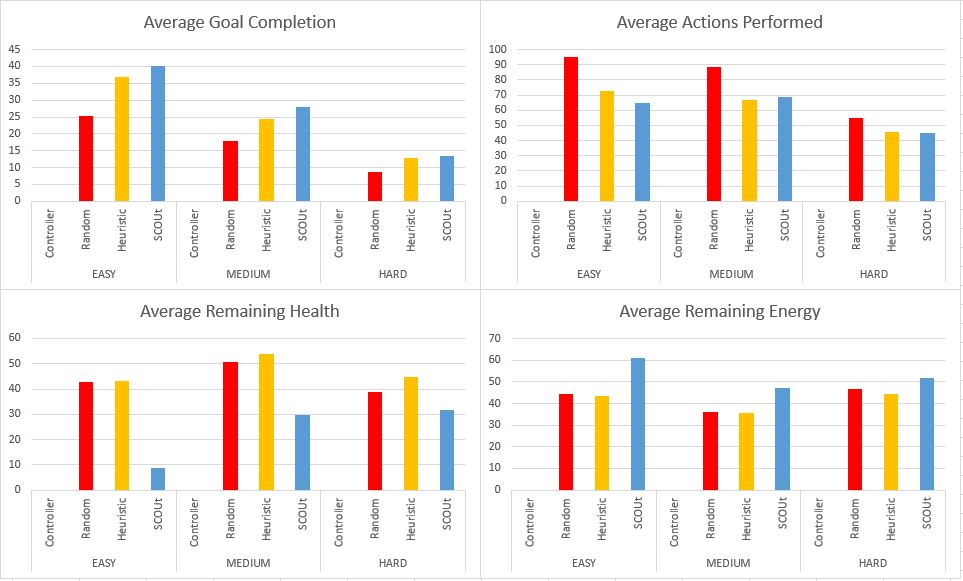
\includegraphics[width=1.0\columnwidth]{Figures/Results/Experiment1/MapWater.JPG}
  \caption{Performance results for $Random$, $Heuristic_{MW}$ and $SCOUt_{MW}$ attempting \textit{Map Water} in various environment difficulties.}
  \label{fig:mapwater_test_results}
\end{figure}


$SCOUt_{H}$ was tested in both \textit{Find Human} and \textit{Map Water}.
The results for each goal type are found in figures~\ref{fig:hybrid_findhuman_test_results} and~\ref{fig:hybrid_mapwater_test_results}, respectively.
Results for \textit{Find Human} operations show trends similar to the results for the $SCOUt_{FH}$ controller, except with smaller margins of increased performance against $Heuristic_{FH}$ and $Random$.
In environments of hard difficulty, $SCOUt_{H}$ shows performance levels that match with the heuristic controller.
This is likely caused by the fact that it was only trained on \textit{Find Human} for 15 iterations, along with a dilution effect caused by having a mixed memory set (from training on both goals).

\begin{figure}[H]
  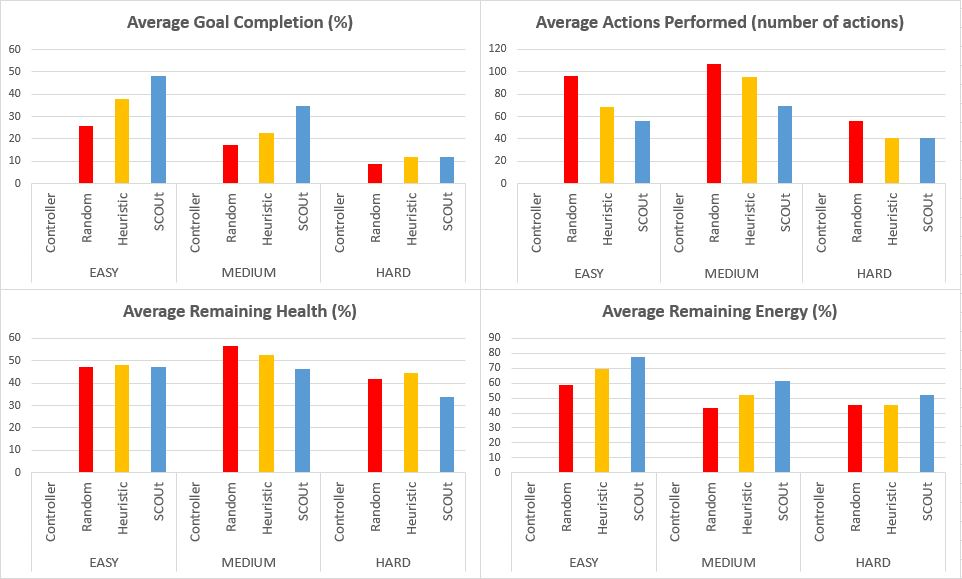
\includegraphics[width=1.0\columnwidth]{Figures/Results/Experiment1/HybridFindHuman.JPG}
  \caption{Performance results for $Random$, $Heuristic_{FH}$ and $SCOUt_{H}$ attempting \textit{Find Human} in various environment difficulties.}
  \label{fig:hybrid_findhuman_test_results}
\end{figure}

Results in \textit{Map Water} for the hybrid controller are nearly identical to the results seen in figure~\ref{fig:mapwater_test_results}.
The only notable difference is that average remaining health in easy environments was \textasciitilde21 percent instead of \textasciitilde9 percent.
Outside of this, performance scores and trends of all three controllers are roughly the same.
This suggests that operations based on mapping an element type are more difficult than would be expected.

\begin{figure}[H]
  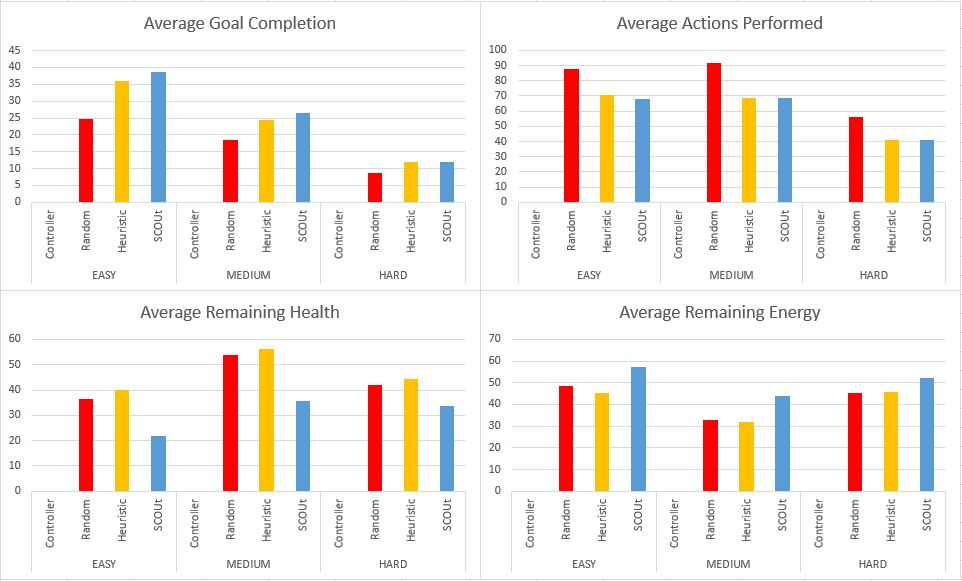
\includegraphics[width=1.0\columnwidth]{Figures/Results/Experiment1/HybridMapWater.JPG}
  \caption{Performance results for $Random$, $Heuristic_{MW}$ and $SCOUt_{H}$ attempting \textit{Map Water} in various environment difficulties.}
  \label{fig:hybrid_mapwater_test_results}
\end{figure}


\section{Experiment 2} \label{sec:experiment2}
The second experiment is broken into three tests: goal changing, sensor set changing, and additional training.
Goal changing, and sensor set changing are both designed to investigate the adaptability of each SCOUt controller.
Heuristic and random controllers are still used as baselines, but we also use SCOUt controllers as a baseline.
By comparing SCOUt controllers that were trained for the specific goal (in the case of goal changing) or un-altered (in the case of sensor set changing), we can study how performance changes when a SCOUt controller is applied in unexpected scenarios.
Following this, $SCOUt_{FH}$ and $SCOUt_{MW}$ are put through additional training on the goal they were not originally trained, to build two new controllers.
$SCOUt_{FH+}$ is the result of training on \textit{Map Water}, beginning with a copy of $SCOUt_{FH}$'s existing memory.
$SCOUt_{MW+}$ is the result of training on \textit{Find Human}, beginning with a copy of $SCOUt_{MW}$'s existing memory.
The new controllers will be tested to see how well SCOUt's control model is able to learn new tasks beginning with separate memory from another task.


\subsection{Goal Changing}
Goal changing tests the performance of $SCOUt_{FH}$ on the \textit{Map Water} goal, and the performance of $SCOUt_{MW}$ on the \textit{Find Human} goal.
The SCOUt controllers have no training on the new goal they are tested within, so behaviors are based purely on the controller's existing memory.
Every controller used in experimentation thus far is compared in these tests.
Tests are run in the same fashion (1000 operations per environment: 200 environments generated, each used 5 times), but in the results we display, performance is averaged for each controller across all three environment difficulties.
This is done because we have already seen that each controller's performance scores show a relatively linear trend as difficulty increases (outside of the case with $SCOUt_{MW}$'s average remaining health).

Results for $SCOUt_{MW}$ in \textit{Find Human} operations are shown in figure~\ref{fig:goal_change_findhuman}.
Unsurprisingly, $SCOUt_{FH}$ takes the lead in every performance category, followed by $SCOUt_{H}$.
What we are primarily interested in here is $SCOUt_{MW}$'s ability to outperform $Heuristic_{FH}$.
We do see higher averages in the number of actions performed and remaining energy, but this is likely due to the same hazard avoidance caveat discussed in Experiment 1 (section~\ref{sec:experiment1}).
This is also reflected in the fact that $SCOUt_{MW}$ has the lowest average remaining health out of all controllers, followed by $SCOUt_{H}$ (again, likely suffering from the same issue).
However, even though the average goal completion for $SCOUt_{MW}$ is less than $Heuristic_{FH}$, the margin of difference is only \textasciitilde1.5 percent.
This does lead to the idea that adaptability is present within SCOUt's control schema.
Using no prior training for how to find a human within an environment, the controller was still able to perform at the same level as a heuristic model.
Additionally, $SCOUt_{MW}$ also outperforms $Heuristic_{MW}$ in all categories excluding average remaining health.
This supports the primary focus of this paper, which is: demonstrating how autonomous control schemas built for one specific task are not inherently adaptable to new tasks, but there still exists underlying features of autonomous control that can be abstracted to create a unified control schema capable of achieving a variety of tasks.

\begin{figure}[H]
  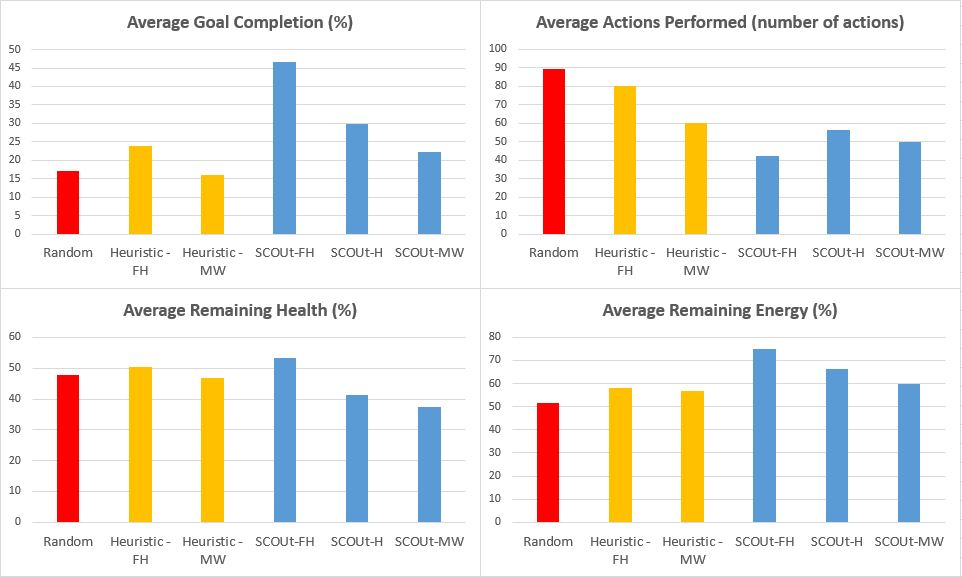
\includegraphics[width=1.0\columnwidth]{Figures/Results/Experiment2/GoalChange/FindHumanGoal.JPG}
  \caption{Results for $SCOUt_{MW}$ in \textit{Find Human} operations compared against $Random$, $Heuristic_{FH}$, $Heuristic_{MW}$, $SCOUt_{FH}$, and $SCOUt_{H}$. While $SCOUt_{MW}$ did not have the best performance results out of all of the SCOUt controllers, it still performed better than $Random$ and both heuristic controllers in the majority of cases. This exemplifies the SCOUt control schema's ability to adapt to new goal types.}
  \label{fig:goal_change_findhuman}
\end{figure}

Goal change tests for the \textit{Map Water} goal (figure~\ref{fig:goal_change_mapwater}) hold some interesting results.
All three SCOUt controllers outperformed $Random$ and both heuristic controllers in every category except for average remaining health.
The fact that even $SCOUt_{FH}$ falls victim to poor performance in hazard avoidance suggests that there is level of inevitability for this control schema to eventually choose a detrimental action.
On the positive side, the goal completion rates for all three show superiority over the other controllers, with $SCOUt_{FH}$ taking the lead.
This could possibly be attributed to $SCOUt_{FH}$ having training where efficient sensor usage is highly rewarded.
Another interesting note is that $Heuristic_{FH}$ follows closely behind $Heuristic_{MW}$ in performance, and even takes the lead in average remaining health.
This speaks more toward the goal at hand than the control schema.
As stated previously in section~\ref{sec:experiment1}, element type mapping is likely a trickier task than expected.
The fact that the range of goal completion of heuristic and SCOUt controllers was ~24 - 28 percent supports this idea.

\begin{figure}[H]
  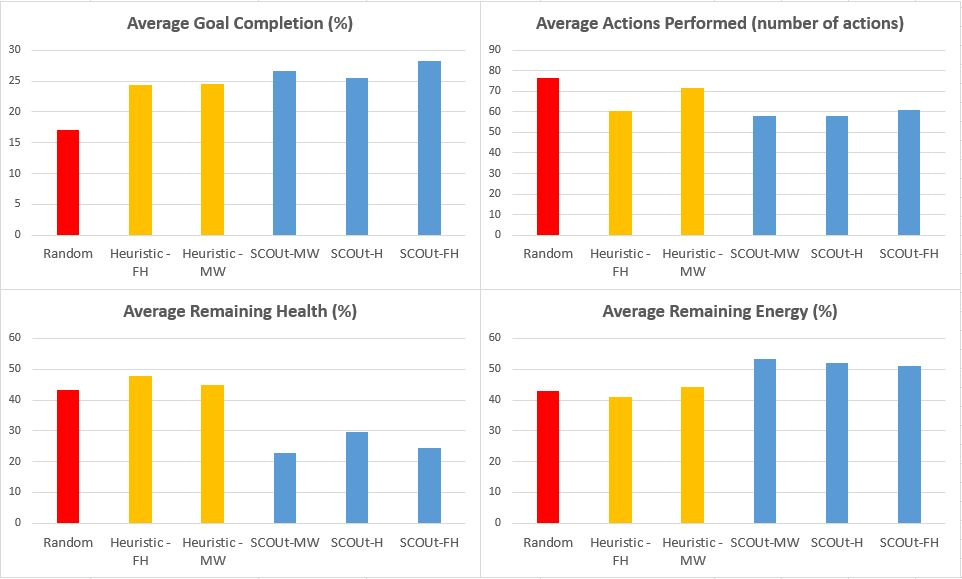
\includegraphics[width=1.0\columnwidth]{Figures/Results/Experiment2/GoalChange/MapWaterGoal.JPG}
  \caption{Results for $SCOUt_{FH}$ in \textit{Map Water} operations compared against $Random$, $Heuristic_{FH}$, $Heuristic_{MW}$, $SCOUt_{MW}$, and $SCOUt_{H}$. Results show that all SCOUt controllers performed at roughly the same level in all categories. In all categories besides average remaining health, the SCOUt controllers perform best. $SCOUt_{FH}$ takes the lead in goal completion out of all controllers. This again supports the adaptability of the SCOUt control schema.}
  \label{fig:goal_change_mapwater}
\end{figure}


\subsection{Sensor Set Changing} \label{sec:sensor_change}
Sensor set changing analyzes how a SCOUt controller is able to perform the goal they were trained for after removing a sensor that it had learned to use for achieving the given task.
Tests are conducted in the same manner as the goal change tests, where 1000 tests per environment difficulty are run, and performance results are averaged across each difficulty level.
The controllers used in each test are $Random$, the heuristic controller designed for the given goal, the original SCOUt controller trained on the goal (denoted as $<controller-name> - All$), and copies of the same SCOUt controller setup with a variation of available sensors.

First, we will examine the results for the \textit{Map Water} goal (figure~\ref{fig:change_sensors_mapwater}).
Because only water and elevation sensors are used in \textit{Map Water} operations (and elimination of the water sensor would result in the inability to achieve any level of goal completion), only one agent variation is considered ($SCOUt_{MW} - No Elevation$).
We see $SCOUt_{MW} - All$ and $SCOUt_{MW} - No Elevation$ topping each performance category besides average remaining health.
$SCOUt_{MW} - No Elevation$ outperforms $SCOUt_{MW} - All$ in each category outside of remaining health.
This is likely due to the fact that $SCOUt_{MW} - No Elevation$ only has a water sensor, and therefore can only choose to scan for water, or move.
The drop in average remaining health could then be attributed to the controller's lack of ability to detect hazardous drops in elevation.
If this is true, it would suggest that SCOUt's ability to learn hazard avoidance is not entirely flawed.

\begin{figure}[H]
  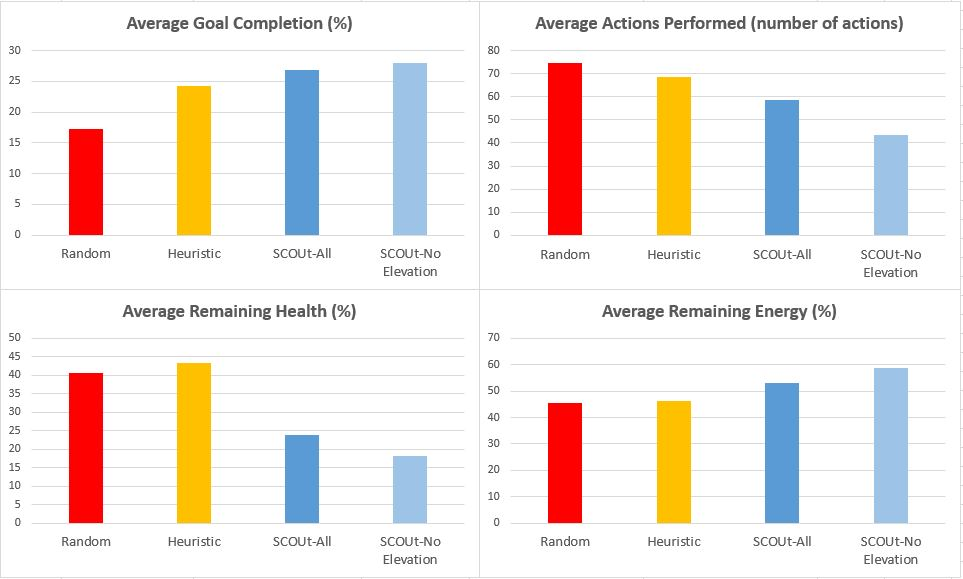
\includegraphics[width=1.0\columnwidth]{Figures/Results/Experiment2/SensorChange/MapWater.JPG}
  \caption{Performance results for $SCOUt_{MW}$ when its elevation sensor was removed ($SCOUt_{MW} - No Elevation$) in \textit{Map Water} operations. It was also compared against an un-altered version of $SCOUt_{MW}$ ($SCOUt_{MW} - All$), $Heuristic_{MW}$, and $Random$. The results show that the SCOUt control schema was able to perform adaptively without the availability of the elevation sensor.}
  \label{fig:change_sensors_mapwater}
\end{figure}

Moving on to testing with the $SCOUt_{FH}$, we see positive results in figure~\ref{fig:change_sensors_findhuman}.
Four variations of sensor sets are examined by removing the elevation, water, temperature and then decibel sensors.
The four respective controllers are denoted as $SCOUt_{FH} - No Elevation$, $SCOUt_{FH} - No Water$, $SCOUt_{FH} - No Temp$ and $SCOUt_{FH} - No Decibel$.
In three out of the four performance categories, the majority of SCOUt controllers perform best.
The only SCOUt controller with a large performance difference among the five is $SCOUt_{FH} - No Decibel$.
Surveillance of decibel values within the environment is a critical behavior to tracking down the location of the human anomaly.
The fact that $SCOUt_{FH} - No Decibel$ shows performance drops demonstrates the ability of SCOUt's control schema to learn pattern recognition behaviors for goal completion.
Despite the handicap of having no decibel sensor, the controller still outperformed $Random$ and $Heuristic_{FH}$ in goal completion, number of actions performed, and remaining energy.
This further demonstrates the adaptability of the SCOUt control schema.
$SCOUt_{FH} - No Decibel$ likely was still able to pick up on the agent using its temperature sensor, which would require the agent to be moved into closer proximity to the human to detect their heat signature.
Removal of each other sensor surprisingly had little to no effect on performance compared to $SCOUt_{FH} - All$.
Performance in all categories aside from remaining health for all of these controllers were roughly double $Heuristic_{FH}$'s and triple $Random$'s.
These results reveal a strong level of adaptability within SCOUt's memory-based reinforcement learning schema when dealing with new agent setups.

\begin{figure}[H]
  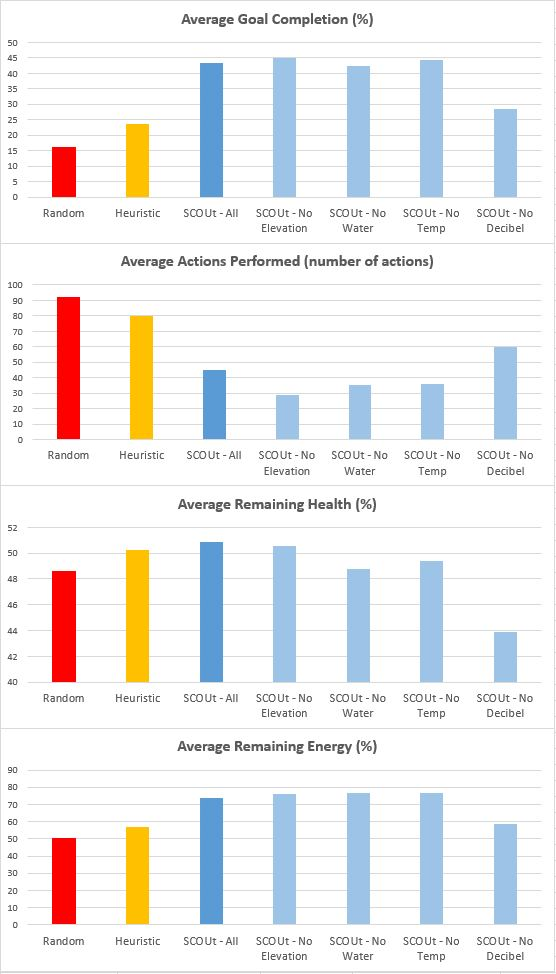
\includegraphics[width=0.75\columnwidth]{Figures/Results/Experiment2/SensorChange/FindHuman.JPG}
  \caption{Performance results for several variations of SCOUt controllers with a sensor removed in \textit{Find Human} operations. These variations were tested against the un-altered SCOUt controller ($SCOUt_{FH}$), $Heuristic_{FH}$, and $Random$. Results show that SCOUt's control schema was able to adapt to each situation where a sensor was removed. The SCOUt controllers outperform $Heuristic_{FH}$ and $Random$ in the majority of performance categories. The only noticeable decline in SCOUt's performance is with the removal of the decibel sensor ($SCOUt_{FH} - No Decibel$). This is likely due to decibel readings being a key indicator of a human's location.}
  \label{fig:change_sensors_findhuman}
\end{figure}


\subsection{Additional Training}
The final task of Experiment 2 was to observe how quickly a controller is able to improve and learn new behaviors related to a different goal.
Two new controllers are retrained and then tested for completing a new goal.
$SCOUt_{FH+}$ begins with a copy of $SCOUt_{FH}$'s trained memory and is then retrained for completing \textit{Map Water}.
$SCOUt_{MW+}$ begins with a copy of $SCOUt_{MW}$'s trained memory and is then retrained for completing \textit{Find Human}.
The retraining for each new controller follows the same setup seen in section~\ref{sec:training}.
Once completed, each controller will be tested in the new goal they were trained against $SCOUt_{FH}$, $SCOUt_{MW}$, the goal's respective heuristic controller, and the $Random$ controller.
We expect to see that the retrained controllers will perform better than the original SCOUt controller whose memory they use.
Additionally, we would like to see measures of performance that are better than the heuristic controller and near the levels of the original SCOUt controller that was trained for the given goal.
Tests are conducted in the same fashion as seen in Change Goal and Change Water testing.
One thousand operations are conducted per environment difficulty and the results are averaged from the total 3000 operations.

Retraining for both new controllers show trends that are similar to all training seen in our original controllers.
$SCOUt_{FH+}$ retraining on \textit{Map Water} (figure~\ref{fig:findhumanplus_training_results}) does not show any increase in goal completion and we see a decline in the average health.
Remaining energy and number of actions performed climb and fall for the same reason discussed with the original $SCOUt_{MW}$ controller, where short operations caused by health depletion reflect in less overall activity.
$SCOUt_{MW+}$ shows major improvement in goal completion while maintaining a low average number of actions taken (seen in figure~\ref{fig:mapwaterplus_training_results}).
Additionally, we see minor climbs in the average remaining health and energy of the agent as it learns to operate more efficiently.


\begin{figure}[H]
  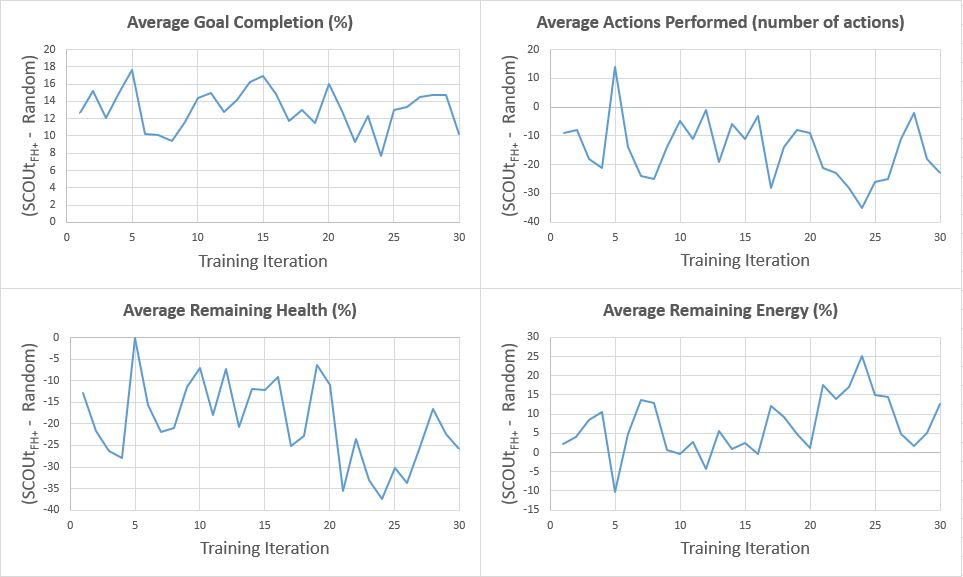
\includegraphics[width=0.9\columnwidth]{Figures/Results/Experiment2/AdditionalTraining/FHPlus_Training.JPG}
  \caption{Iteration testing performance results for $SCOUt_{FH+}$ attempting \textit{Map Water}. All graphs show the controller's average difference in performance compared to $Random$ ($SCOUt_{FH+}$ average - $Random$ average) VS the number of training iterations completed.}
  \label{fig:findhumanplus_training_results}
\end{figure}

\begin{figure}[H]
  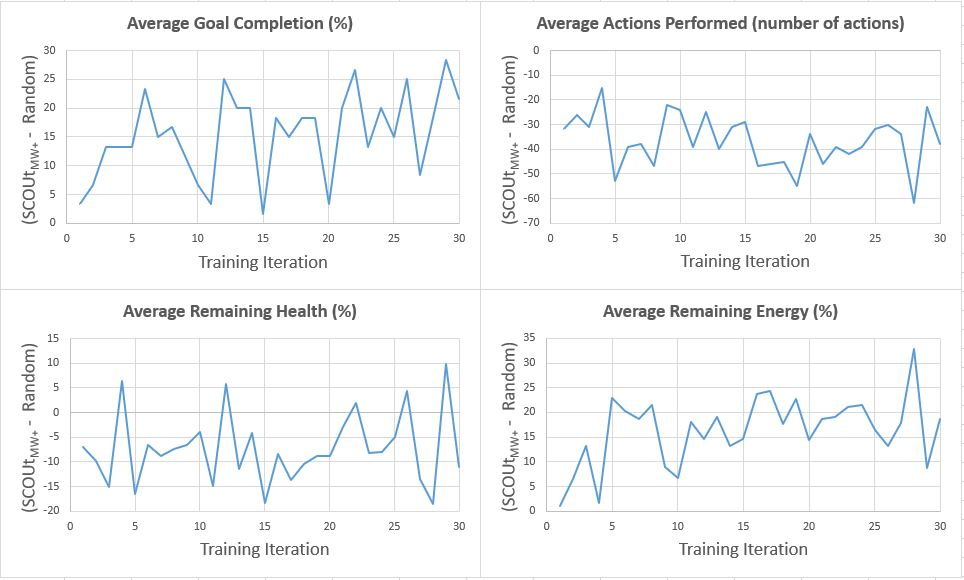
\includegraphics[width=0.9\columnwidth]{Figures/Results/Experiment2/AdditionalTraining/MWPlus_Training.JPG}
  \caption{Iteration testing performance results for $SCOUt_{MW+}$ attempting \textit{Map Water}. All graphs show the controller's average difference in performance compared to $Random$ ($SCOUt_{MW+}$ average - $Random$ average) VS the number of training iterations completed.}
  \label{fig:mapwaterplus_training_results}
\end{figure}


After training, $SCOUt_{FH+}$ was tested for performance in \textit{Map Water} operations against the original $SCOUt_{FH}$, $SCOUt_{MW}$, $Heuristic_{MW}$, and $Random$.
The results seen in figure~\ref{fig:findhumanplus_test_results} show minor improvements over $SCOUt_{FH}$ for goal completion.
Remaining health is slightly lower, but the number actions taken and remaining energy where still equivalent to that of $SCOUt_{FH}$.
Again, we see another SCOUt controller outranking the $Heuristic_{MW}$ controller designed specifically for the goal at hand in all categories except remaining health.
While hazard avoidance is still an issue, it can still be argued that this controller is operating efficiently as it shows better performance averages in all other categories.

\begin{figure}[H]
  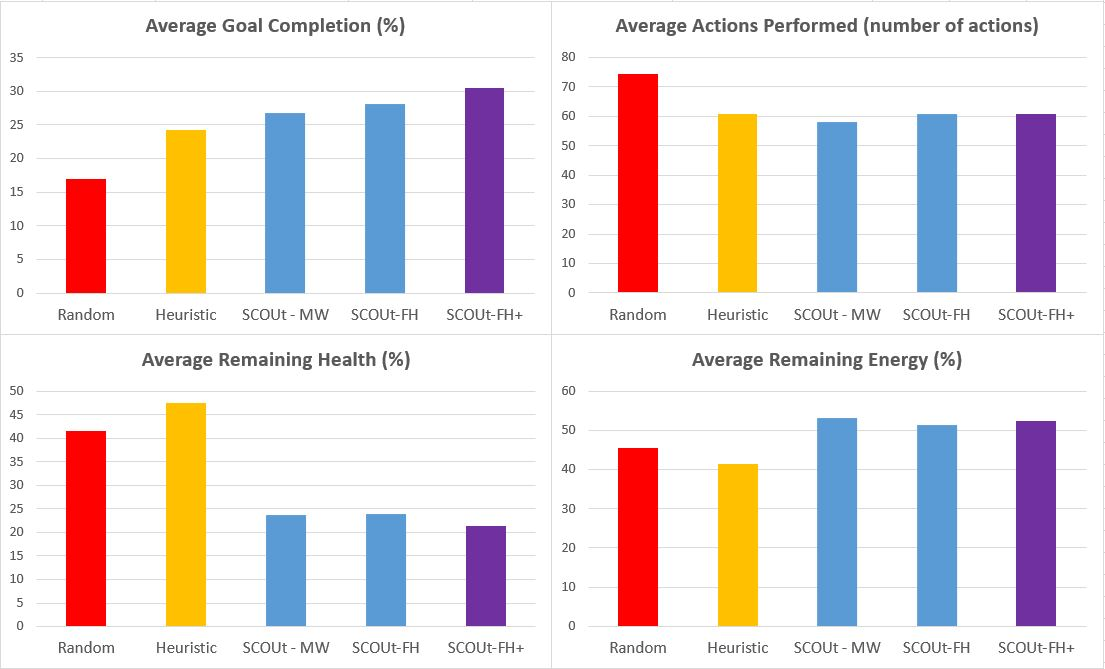
\includegraphics[width=1.0\columnwidth]{Figures/Results/Experiment2/AdditionalTraining/FindHumanPlus.JPG}
  \caption{Iteration testing performance results for $SCOUt_{FH+}$ attempting \textit{Map Water}. All graphs show the controller's average difference in performance compared to $Random$ ($SCOUt_{FH+}$ average - $Random$ average) VS the number of training iterations completed.}
  \label{fig:findhumanplus_test_results}
\end{figure}


Figure~\ref{fig:mapwaterplus_test_results} shows the performance of $SCOUt_{MW+}$ against the original $SCOUt_{MW}$, $SCOUt_{FH}$, $Heuristic_{FH}$, and $Random$ in \textit{Find Human} operations.
Here we see that $SCOUt_{MW+}$ does outrank $SCOUt_{MW}$ and the heuristic controller as expected.
$SCOUt_{FH}$ still takes the lead in every category, but the new controller does show major overall improvements due to its additional training.
This further supports the argument that a memory-based reinforcement learning model holds many adaptive attributes for facing new situations.


\begin{figure}[H]
  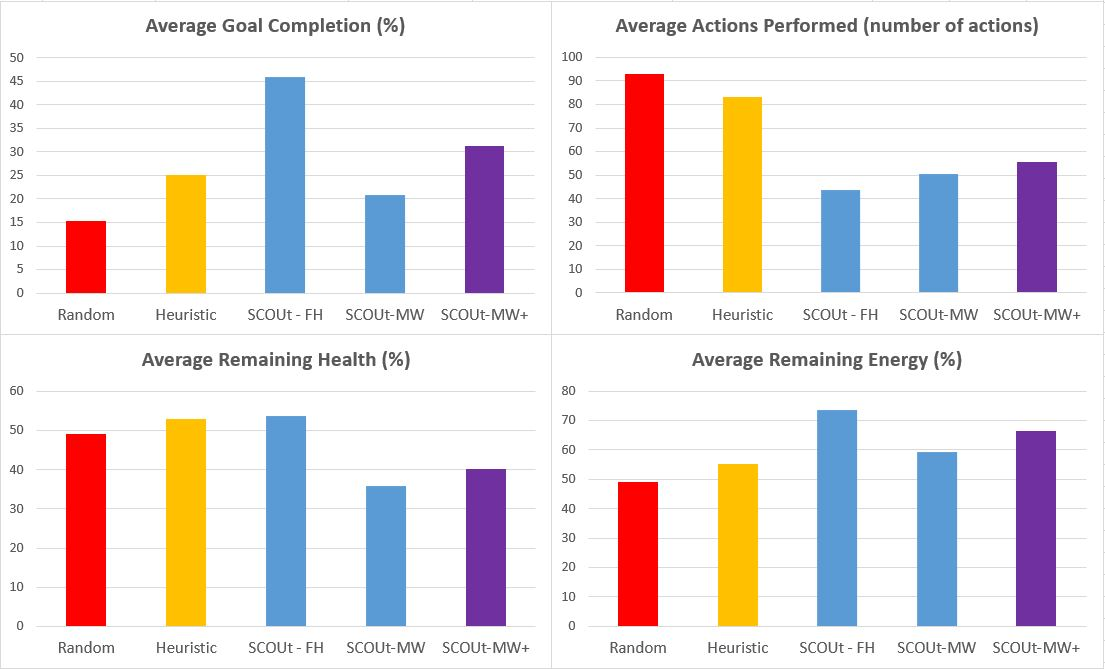
\includegraphics[width=1.0\columnwidth]{Figures/Results/Experiment2/AdditionalTraining/MapWaterPlus.JPG}
  \caption{Iteration testing performance results for $SCOUt_{MW+}$ attempting \textit{Map Water}. All graphs show the controller's average difference in performance compared to $Random$ ($SCOUt_{MW+}$ average - $Random$ average) VS the number of training iterations completed.}
  \label{fig:mapwaterplus_test_results}
\end{figure}



\section{Discussion}
Our testing revealed that SCOUt's control schema was in fact adaptive to new tasks.
In Experiment 2, we see SCOUt controllers performing better than random and heuristic approaches, even when faced with disadvantages, such as lack of sensors or no knowledge of how to complete a goal.
These are features that we don't see in our heuristic models.
The heuristic approaches were able to perform adequately in their respective goals, but due to the goal-specific logic that was used in their control models, they did not perform well when presented to a new goal type.
We do see an issue with SCOUt's hazard avoidance, as results in all testing showed poor ranking in the category of average remaining health.
Despite this, SCOUt still showed superior results in the other three categories for the majority of tests.
It is suspected that if the hazard avoidance issue were to be fixed, we would see even better results in all performance categories.
Another notable feature within our results was $SCOUt_{FH}$'s performance in the goal change testing (figure~\ref{fig:goal_change_findhuman}).
Here we saw that the SCOUt controller without a decibel sensor equipped showed noticeable performance drops, but still performed better than the random and heuristic controllers.
This signifies two things.
First, SCOUt is learning behaviors related to goal completion.
Changes in decibel levels within the environment are the strongest indicator to finding a human's location.
The fact that $SCOUt_{FH} - No Decibel$ showed lower performance compared to all other SCOUt controllers in the test suggests that the controller has learned search behaviors related to analyzing the environment.
Second, because SCOUt was still able to outperform the random and heuristic controllers despite its disadvantage in this situation, we argue that SCOUt's control model is in fact adaptive.
While $SCOUt_{FH} - No Decibel$ would not be able to pick up on the human's sound effect, it was able to use other learned information to still guide it to successfully goal completions.



\chapter{Conclusion}
Conclude stuff

% 

\chapter{Future Work}
How to improve this approach.


\bibliographystyle{plain}
\bibliography{References}



% Code settings
\lstset{
  language=Scala, % C, C++, Java, SQL are from the around hundred available
  basicstyle=\ttfamily,
  numbers=left,
  numberstyle=\footnotesize,
  stepnumber=1,
  numbersep=2.0mm,
  breaklines=true}


\chapter{APPENDIX} \label{appendix}

\section{Appendix A: Code Listings} \label{code_listings}
This appendix contains all code listings referenced within the paper.



\subsection{Environment Data Structures} \label{appendix:environment_data_structures}
This section covers all data structures related to an environment.
Together these traits, classes, and instances can be combined in different ways to create unique models of real-world environments.

\begin{appx}
  \caption{A class for representing a real-world environment. It is laid out in a grid of cells that contain information related to each of their respective areas within the grid.}
  \lstinputlisting{Codes/Environment.scala} \label{appendix:environment_class}
\end{appx}


\begin{appx}
  \caption{A class that represents a sub-section of an environment. The data stored in each instance represents the features that are found within the \texttt{Cell}'s area within the environment.}
  \lstinputlisting{Codes/Cell.scala} \label{appendix:cell_class}
\end{appx}


\begin{appx}
  \caption{An \texttt{Element} trait is a generalized representation of a measurable feature type within an environment. Specific element types can be created by extending this trait. Each instance defines specific information about what values can be represented for the specific element type.}
  \lstinputlisting{Codes/Element.scala} \label{appendix:elelment_trait}
\end{appx}


\begin{appx}
  \caption{\texttt{Elevation} is a class which extends the \texttt{Element} trait. This class models elevation levels within an environment. Different instances can be created to specify a level of elevation for each cell in an environment.}
  \lstinputlisting{Codes/Elevation.scala} \label{appendix:elevation_class}
\end{appx}


\begin{appx}
  \caption{An \texttt{Anomaly} is any object within an environment that may be of interest. Anomalies often have a set of effects that will alter the environment around them. This trait can be extended to define specific types of anomalies that can be represented in an environment.}
  \lstinputlisting{Codes/Anomaly.scala} \label{appendix:anomaly_trait}
\end{appx}

\begin{appx}
  \caption{The \texttt{Effect} trait is a generalized description of an alteration that an \texttt{Anomaly} has on the environment. Effects will alter a single element type in an area of the environment that the anomaly is located within.}
  \lstinputlisting{Codes/Effect.scala} \label{appendix:effect_trait}
\end{appx}

\begin{appx}
  \caption{\texttt{Human} is a specific \texttt{Anomaly} class. This class represents a peron that could be found in an environment. Human's have two defined \texttt{Effects}: sound and heat. These effects will alter the decibel and temperature element values in the human's general area within the environment.}
  \lstinputlisting{Codes/Human.scala} \label{appendix:human_class}
\end{appx}

\begin{appx}
  \caption{A \texttt{Layer} holds a collection of instances of a specific \texttt{Element} class. The collection is represented as a 2-dimentional grid that is relative to an \texttt{Environment} grid. They can be thought of as the same structure as an environment, but only containing information about a single element type.}
  \lstinputlisting{Codes/Layer.scala} \label{appendix:layer_class}
\end{appx}






\subsection{Agent Data Structures}
This section contains data structures that are representative of an agent.
These structures model the different capabilities an agent has to interact with an environment.


\begin{appx}
  \caption{An \texttt{Agent} represents a physical member capable of acting within an environment. The class defines a controller for selecting actions, sensors that the agent is equipped with, mobility and durability features of the agent for modeling interactions with an environment, and several internal status variables.}
  \lstinputlisting{Codes/Agent.scala} \label{appendix:agent_class}
\end{appx}


\begin{appx}
  \caption{A \texttt{Sensor} is a tool that an agent can utilize to collect data about a specific element type within an environment. Sensors have a set range and energy cost related to using them.}
  \lstinputlisting{Codes/Sensor.scala} \label{appendix:sensor_class}
\end{appx}


\begin{appx}
  \caption{\texttt{Mobility} contains a set of variables related to how an agent will be able to safely move within an environment.}
  \lstinputlisting{Codes/Mobility.scala} \label{appendix:mobility_class}
\end{appx}


\begin{appx}
  \caption{\texttt{Durability} defines how an agent will interact with an element type in an environment. Different agents will each have strengths and weaknesses defined by how they will react when in contact with certain elements in an environment.}
  \lstinputlisting{Codes/Durability.scala} \label{appendix:durability_class}
\end{appx}


\begin{appx}
  \caption{An \texttt{AgentState} represents an instance of the internal status of an agent and the information that the agent knows about its environment. An \texttt{Agent}'s internal map is condensed into a set of sub-states within the entire agent state for each element type that the agent has knowledge of.}
  \lstinputlisting{Codes/AgentState.scala} \label{appendix:agentstate_class}
\end{appx}


\begin{appx}
  \caption{\texttt{ElementState}s are representative of an agent's knowledge of a specific element type in an environment. The information contained is directly related to what the agent has gathered into its internal map through the use a sensor. Specific known values of the element type are divided into four quadrants relative to the agent's current position.}
  \lstinputlisting{Codes/ElementState.scala} \label{appendix:elementstate_class}
\end{appx}


\begin{appx}
  \caption{A \texttt{QuadrantState} represents a collection of known information about a specific element type in a sub-set of cells within an environment. The data is condensed to an average known value differential and immediate known value differential relative to the value in the cell that the agent currently occupies.}
  \lstinputlisting{Codes/QuadrantState.scala} \label{appendix:quadrantstate_class}
\end{appx}


\begin{appx}
  \caption{\texttt{Controller}s are the decision-making models that are used to select actions for an agent to take. The process that each controller uses to select an action vary, but must choose from a set of valid actions and can use information that the agent has gathered while exploring the environment.}
  \lstinputlisting{Codes/Controller.scala} \label{appendix:controller_trait}
\end{appx}



\subsection{Environment Generation Data Structures}
This section includes the data structures used to guide the procedural generation of unique environments.

\begin{appx}
  \caption{\texttt{EnvironmentTemplate}s hold the entire collection of attributes that are used to guide the process of generating an environment.}
\lstinputlisting{Codes/EnvironmentTemplate.scala} \label{appendix:environmenttemplate_class}
\end{appx}


\begin{appx}
  \caption{\texttt{ElementSeed} is a trait used to define helper classes for specific \texttt{Element} classes. They have a set of attributes that can be set to guide how the element type will be initialized in an environment and functions related to the actual process in which the element type will be procedurally generated within the environment.}
\lstinputlisting{Codes/ElementSeed.scala} \label{appendix:elementseed_trait}
\end{appx}


\begin{appx}
  \caption{A \texttt{TerrainModification} is a trait used for defining processes to alter element types within the environment. These help to add unique features within element types found in the environment.}
\lstinputlisting{Codes/TerrainModification.scala} \label{appendix:terrainmodification_trait}
\end{appx}





\subsection{State Comparison Data Structures}
This section includes data structures related to comparing multiple \texttt{AgentState}s to each other.

\begin{appx}
  \caption{\texttt{GaussianData} holds the mean and standard deviation of a collection of values.}
\lstinputlisting{Codes/GaussianData.scala} \label{appendix:gaussian_data}
\end{appx}


\begin{appx}
  \caption{\texttt{StateActionDifference} holds values related to a comparison that was made between a current \texttt{AgentState} and an \texttt{AgentState} within SCOUt's memory of state-action rewards. Each instance defines the differences that were calculated between two states, an overall state difference, the action that was taken by the agent in the state-action reward, and then the short-term and long-term rewards that the were received for the action.}
\lstinputlisting{Codes/StateActionDifference.scala} \label{appendix:state_action_difference}
\end{appx}








\subsection{Experimentation Setup} \label{appendix:experiment_setup}
This section includes the code listings for the \texttt{Agent} configuration and \texttt{EnvironmentTemplate}s used in experimentation.

\begin{appx}
  \caption{Instances of the \texttt{Agent} class and \texttt{Sensor} classes that are used in experimentation. Some attributes are set per operation during experiments. These are marked with a comment ``Defined Per Operation.''}
  \lstinputlisting{Codes/TestAgentSetup.scala} \label{appendix:agent_setup}
\end{appx}

\begin{appx}
  \caption{JSON data storing the an environment template used in experimentation. This template is title \textit{EASY} as it represents a relatively easy environment for an operation to take place in. The environment is $8\times8$ cells and contains only one modification for a pool of water to be generated within the environment.}
  \lstinputlisting[language=Java]{Codes/EASY.json} \label{appendix:easy_environmenttemplate}
\end{appx}

\begin{appx}
  \caption{JSON data storing the an environment template used in experimentation. This template is title \textit{MEDIUM} as it presents a few challenging features that an agent may face. The environment is $10\times10$ cells and contains both a ``hill'' elevation modification and a water pool modification. Compared to the \textit{EASY} environment template, \textit{MEDIUM} has higher ambient levels of decibel and temperature values, making it slightly more difficult to identify the effects of a human anomaly within the environment.}
  \lstinputlisting[language=Java]{Codes/MEDIUM.json} \label{appendix:easy_environmenttemplate}
\end{appx}

\begin{appx}
  \caption{JSON data storing the an environment template used in experimentation. This template is title \textit{HARD} as it presents many challenging features that an agent may face. The environment is $12\times12$ cells and contains a ``hill'' elevation modification, a ``valley'' elevation modification, a water pool modification, and a water stream modification. Additionally, the ambient levels of decibel values and temperature values are raised and the sound and heat effects of the human anomaly are suppressed even more than seen in the \textit{MEDIUM} environment template. The combination of all of these factors create environments that are both highly difficult to safely navigate and difficult to identify anomaly effects within.}
  \lstinputlisting[language=Java]{Codes/HARD.json} \label{appendix:easy_environmenttemplate}
\end{appx}




%--------------------------------------------------------------------------
% BEGIN FIGURES
%--------------------------------------------------------------------------
\section{Appendix B: Additional Figures} \label{appendix:additional_figures}
This appendix holds all figures that were not placed in the main body of the paper.

\subsection{Training Variation 1}
This section contains results for our first variation of training the three SCOUt controller memories ($SCOUt_{FH}$, $SCOUt_{MW}$, and $SCOUt_{H}$).
During training and iteration testing, the long-term reward (algorithm~\ref{algorithmic:long_term_reward}) was adjusted to only factor in a \texttt{goalReward} if the agent had remaining health at the end of an operation.
This was done to observe how SCOUt controllers would change the agent's behavior when their memory of state-action rewards reflected smaller long-term rewards from operations where the agent's health was depleted.
It was hoped that we would see better performance in average remaining energy and subsequently all other areas.
However, we found no significant improvements in performance.
Appendix~\ref{appendix:findhuman_training_variation1} shows the results for $SCOUt_{FH}$, Appendix~\ref{appendix:mapwater_training_variation1} shows the results for $SCOUt_{MW}$, and Appendix~\ref{appendix:hybrid_training_fh_variation1} and~\ref{appendix:hybrid_training_mw_variation1} show results for $SCOUt_{H}$ in \textit{Find Human} and \textit{Map Water} operations, respectively.

\begin{appx}
\begin{figure}[H]
  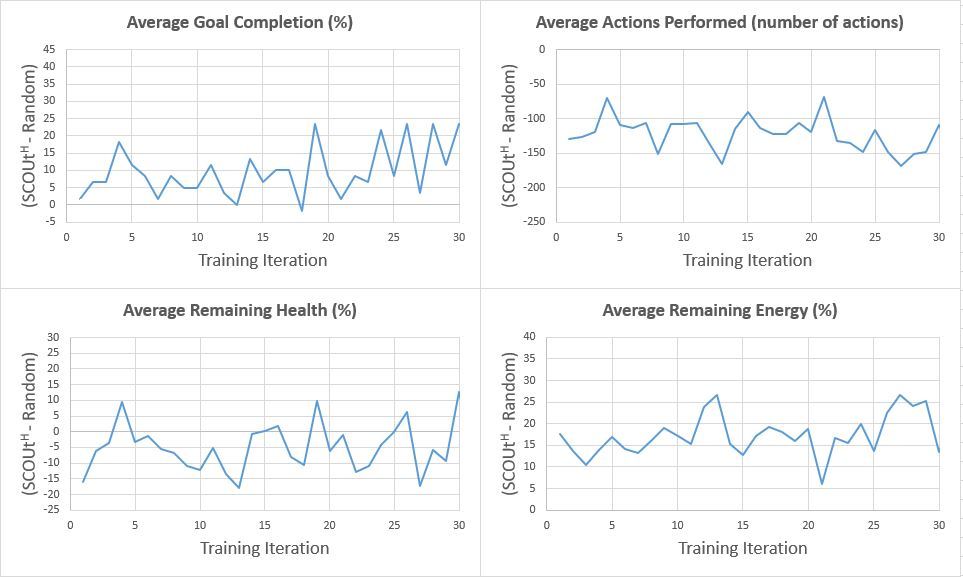
\includegraphics[width=0.9\columnwidth]{Figures/Results/TrainingVariation1/FindHuman.JPG}
  \caption{Iteration testing performance results for $SCOUt_{FH}$ attempting \textit{Find Human} using setup variation 1 (see subsection~\ref{subsec:training_variations}). All graphs show the controller's average difference in performance compared to $Random$ ($SCOUt_{FH}$ average - $Random$ average) VS the number of training iterations completed.}
  \label{appendix:findhuman_training_variation1}
\end{figure}
\end{appx}


\begin{appx}
\begin{figure}[H]
  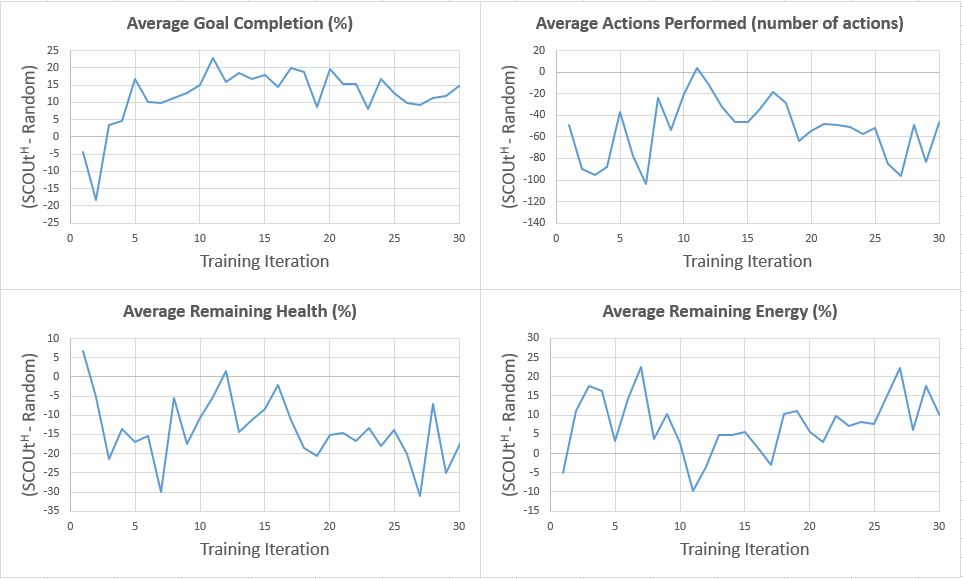
\includegraphics[width=0.9\columnwidth]{Figures/Results/TrainingVariation1/MapWater.JPG}
  \caption{Iteration testing performance results for $SCOUt_{MW}$ attempting \textit{Map Water} using setup variation 1 (see subsection~\ref{subsec:training_variations}). All graphs show the controller's average difference in performance compared to $Random$ ($SCOUt_{MW}$ average - $Random$ average) VS the number of training iterations completed.}
  \label{appendix:mapwater_training_variation1}
\end{figure}
\end{appx}


\begin{appx}
\begin{figure}[H]
  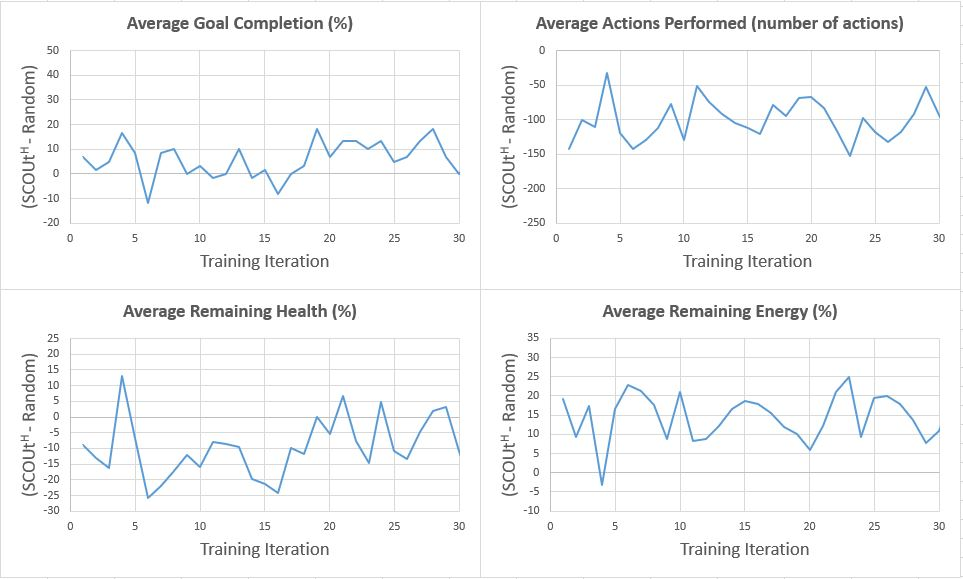
\includegraphics[width=0.9\columnwidth]{Figures/Results/TrainingVariation1/Hybrid-FindHuman.JPG}
  \caption{Iteration testing performance results for $SCOUt_{H}$ attempting \textit{Find Human} using setup variation 1 (see subsection~\ref{subsec:training_variations}). All graphs show the controller's average difference in performance compared to $Random$ ($SCOUt_{H}$ average - $Random$ average) VS the number of training iterations completed.}
  \label{appendix:hybrid_training_fh_variation1}
\end{figure}
\end{appx}


\begin{appx}
\begin{figure}[H]
  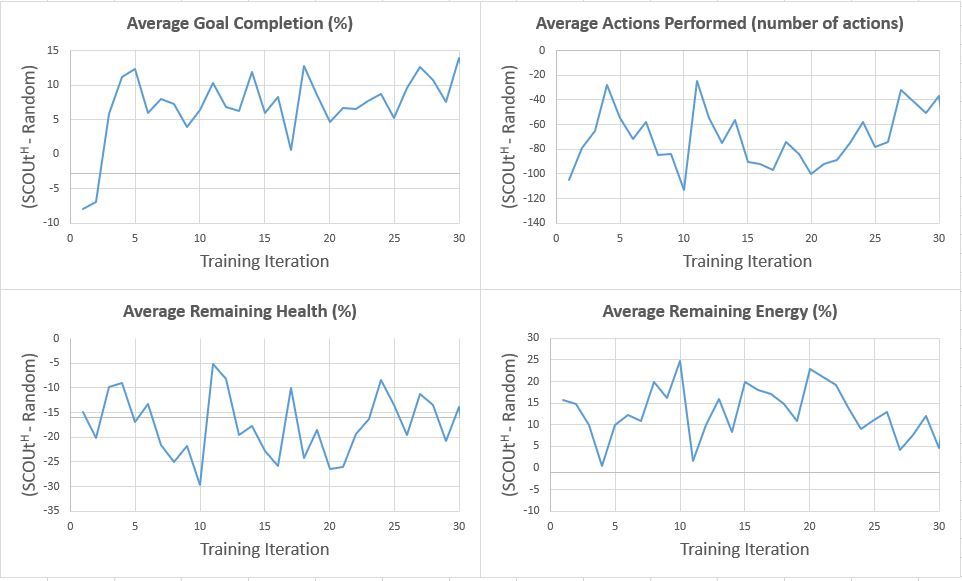
\includegraphics[width=0.9\columnwidth]{Figures/Results/TrainingVariation1/Hybrid-MapWater.JPG}
  \caption{Iteration testing performance results for $SCOUt_{H}$ attempting \textit{Map Water} using setup variation 1 (see subsection~\ref{subsec:training_variations}). All graphs show the controller's average difference in performance compared to $Random$ ($SCOUt_{H}$ average - $Random$ average) VS the number of training iterations completed.}
  \label{appendix:hybrid_training_mw_variation1}
\end{figure}
\end{appx}



\subsection{Training Variation 2}
This section contains results for our second variation of training the three SCOUt controller memories ($SCOUt_{FH}$, $SCOUt_{MW}$, and $SCOUt_{H}$).
During training and iteration testing, the \textit{goalRewardWeight} used for calculating long-term reward (algorithm~\ref{algorithmic:long_term_reward}) was set to 1.5.
This was done to observe how SCOUt controllers would change the agent's behavior when their memory of state-action rewards reflected a stronger emphasis on the level of goal completion attained.
It was hoped that we would see better performance in all categories.
While only slight improvements were observed, this method was chosen for all testing conducted in our experimentation.
Appendix~\ref{appendix:findhuman_training_variation2} shows the results for $SCOUt_{FH}$, Appendix~\ref{appendix:mapwater_training_variation2} shows the results for $SCOUt_{MW}$, and Appendix~\ref{appendix:hybrid_training_fh_variation2} and~\ref{appendix:hybrid_training_mw_variation2} show results for $SCOUt_{H}$ in \textit{Find Human} and \textit{Map Water} operations, respectively.

\begin{appx}
\begin{figure}[H]
  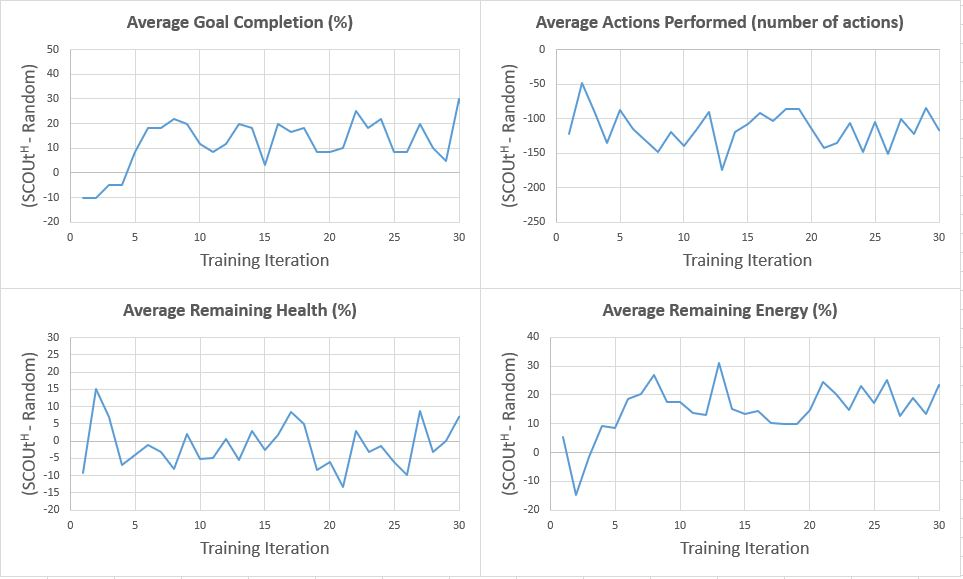
\includegraphics[width=0.9\columnwidth]{Figures/Results/TrainingVariation2/FindHuman.JPG}
  \caption{Iteration testing performance results for $SCOUt_{FH}$ attempting \textit{Find Human} using setup variation 2 (see subsection~\ref{subsec:training_variations}). All graphs show the controller's average difference in performance compared to $Random$ ($SCOUt_{FH}$ average - $Random$ average) VS the number of training iterations completed.}
  \label{appendix:findhuman_training_variation2}
\end{figure}
\end{appx}


\begin{appx}
\begin{figure}[H]
  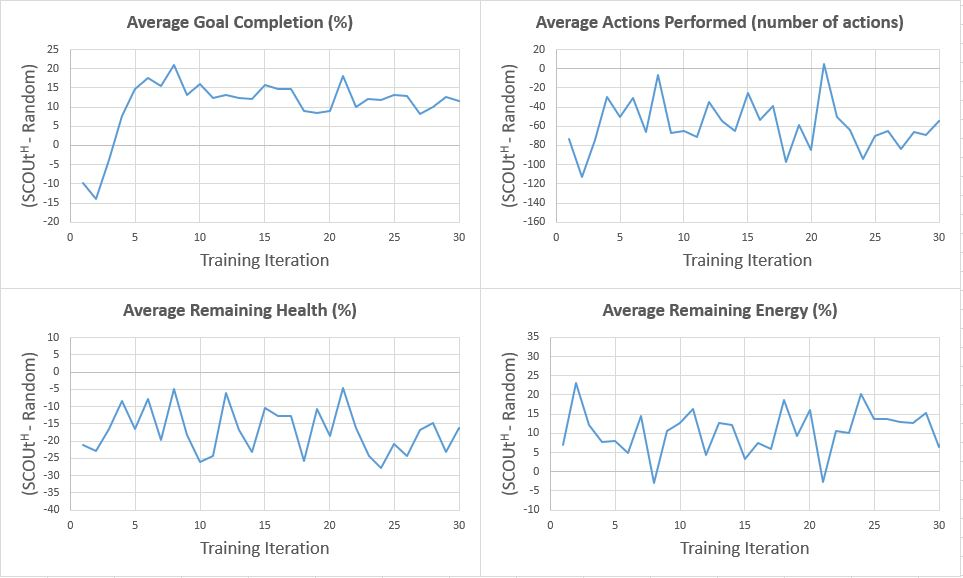
\includegraphics[width=0.9\columnwidth]{Figures/Results/TrainingVariation2/MapWater.JPG}
  \caption{Iteration testing performance results for $SCOUt_{MW}$ attempting \textit{Map Water} using setup variation 2 (see subsection~\ref{subsec:training_variations}). All graphs show the controller's average difference in performance compared to $Random$ ($SCOUt_{MW}$ average - $Random$ average) VS the number of training iterations completed.}
  \label{appendix:mapwater_training_variation2}
\end{figure}
\end{appx}


\begin{appx}
\begin{figure}[H]
  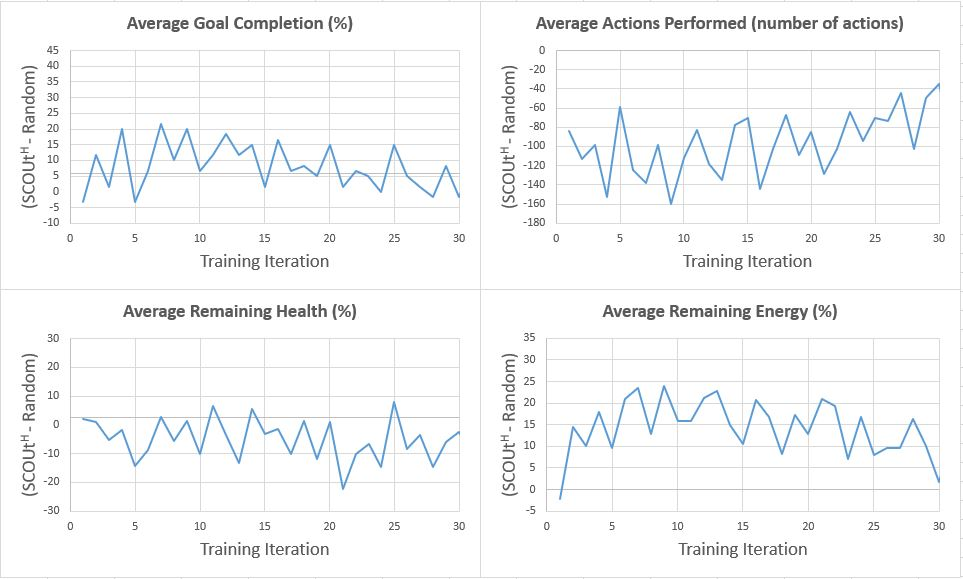
\includegraphics[width=0.9\columnwidth]{Figures/Results/TrainingVariation2/Hybrid-FindHuman.JPG}
  \caption{Iteration testing performance results for $SCOUt_{H}$ attempting \textit{Find Human} using setup variation 2 (see subsection~\ref{subsec:training_variations}). All graphs show the controller's average difference in performance compared to $Random$ ($SCOUt_{H}$ average - $Random$ average) VS the number of training iterations completed.}
  \label{appendix:hybrid_training_fh_variation2}
\end{figure}
\end{appx}


\begin{appx}
\begin{figure}[H]
  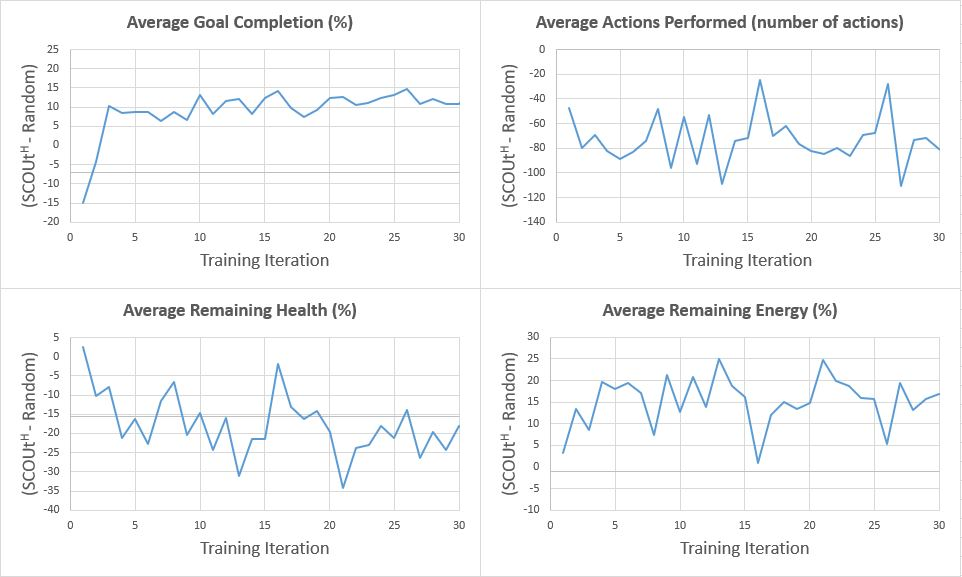
\includegraphics[width=0.9\columnwidth]{Figures/Results/TrainingVariation2/Hybrid-MapWater.JPG}
  \caption{Iteration testing performance results for $SCOUt_{H}$ attempting \textit{Map Water} using setup variation 2 (see subsection~\ref{subsec:training_variations}). All graphs show the controller's average difference in performance compared to $Random$ ($SCOUt_{H}$ average - $Random$ average) VS the number of training iterations completed.}
  \label{appendix:hybrid_training_mw_variation2}
\end{figure}
\end{appx}





%
% \section{Appendix C: Mathematical Proofs} \label{appendix:proofs}
% This appendix contains mathematical proofs related to the use of Gaussian normalization on value sets.
%
%
%
% \begin{algorithm}[H]
%   \setstretch{1.35}
%   \caption{Proof that...}
%   \begin{algorithmic} \label{appendix:gaussian_difference_identical}
%     \REQUIRE $mean \leftarrow 10$
%     \REQUIRE $sd \leftarrow 1$
%     \REQUIRE $x = y$
%     \ENSURE $x_{normal} = y_{normal}$
%     \STATE $x_{normal} \leftarrow (x - mean) / sd$
%     \STATE $x = y$
%     \STATE $x = y$
%     \STATE $x = y$
%     \STATE $x = y$
%     \STATE $x = y$
%
%   \end{algorithmic}
% \end{algorithm}
%
%
% \begin{lstlisting}[label=appendix:gaussian_difference_identical]
% Example:
% Gaussian mean = 10
% Gaussian standard deviation = 1
%
% x = 12
% y = 12
% x = y
%
% x(normalized) = (x - Gaussain mean) / Gaussian standard deviation
% x(normalized) = (12 - 10) / 1
% x(normalized) = 2 / 1
% x(normalized) = 2
%
% y(normalized) = (y - Gaussain mean) / Gaussian standard deviation
% y(normalized) = (12 - 10) / 1
% y(normalized) = 2 / 1
% y(normalized) = 2
%
% x(normalized) = y(normalized)
%
% Gaussian difference (x,y) = |x - y|
% Gaussian difference (x,y) = |2 - 2|
% Gaussian difference (x,y) = 0
% \end{lstlisting}
%
%
% \begin{lstlisting}[label=appendix:gaussian_difference_different]
% Example:
% Gaussian mean = 10
% Gaussian standard deviation = 1
%
% x = 12
% y = 7
%
% x(normalized) = (x - Gaussain mean) / Gaussian standard deviation
% x(normalized) = (12 - 10) / 1
% x(normalized) = 2 / 1
% x(normalized) = 2
%
% y(normalized) = (y - Gaussain mean) / Gaussian standard deviation
% y(normalized) = (7 - 10) / 1
% y(normalized) = -3 / 1
% y(normalized) = -3
%
% Gaussian difference (x,y) = |x - y|
% Gaussian difference (x,y) = |2 - -3|
% Gaussian difference (x,y) = 5
% \end{lstlisting}


\end{document}
